\documentclass[parskip,12pt,headsepline,a4paper] {scrbook}

	%%%%%% BEGIN Text related %%%%%%
	\usepackage[latin1]{inputenc} % Umlaute
	\usepackage[T1]{fontenc} % bessere Fontcodierung
	\usepackage[english]{babel} %English language
	\usepackage{textcomp} % Anfuehrungszeichen
	\usepackage{titlesec}

	\parindent0cm	%Kein Einzug bei Absaetzen
	%%%%%% END Text related %%%%%%

	\usepackage{braket}


	%%%%%% BEGIN Graphix, Figures, Tables and Math %%%%%%
	\usepackage{graphicx,hyperref,latexsym,dcolumn}

	\usepackage{float}
	\restylefloat{figure}

	\usepackage[table]{xcolor}
	\usepackage{array} % to use tabular environment

	\usepackage{mathbbol,amssymb,amstext,amsmath} % Mathe
	%%%%%% END Graphix, Figures, Tables and Math %%%%%%


	%%%%%% BEGIN miscellaneous  %%%%%%
	\usepackage{units}
	\usepackage{pdfpages} % to include pdf pages
	\usepackage{listings}

	\usepackage{scrhack} % solves some scrbook errors

	\graphicspath{{img/}} % where to find the graphics

	\newcommand{\changefont}[3]{\fontfamily{#1} \fontseries{#2} \fontshape{#3} \selectfont}

	\pagenumbering{arabic}
	%%%%%% END miscellaneous  %%%%%%

	\usepackage{url}
	%%%%%% BEGIN Bibtex %%%%%%
	%\usepackage{bibtex}
	%\usepackage[numbers]{natbib}
	%\usepackage{bibgerm}
	%%%%%% END Bibtex %%%%%%


	\usepackage{color}
	%%%%%% BEGIN Defining user colors using the HTML,RGB model %%%%%%
	\definecolor{gruen}{HTML}{92F641}
	\definecolor{dunkelgrau}{rgb}{0.87,0.87,0.87}
	\definecolor{hellgrau}{rgb}{0.93,0.93,0.93}
	%%%%%% END Defining user colors using the HTML,RGB model %%%%%%


	%%%%%% BEGIN Format page %%%%%%
	\topmargin=-0.4in \evensidemargin=-12pt \oddsidemargin=12pt
	\setlength{\topskip}{0.4in}
	\textwidth = 16cm \textheight=23.5cm
	%%%%%% END Format page %%%%%%

	\usepackage{setspace}
	\renewcommand{\baselinestretch}{1.2}

	%%%%%% BEGIN Format chapters %%%%%%
	\usepackage{titlesec} % to use titleformat
	%%\renewcommand{\thechapter}{\Roman{chapter}}
	\titleformat{\chapter}[display]
	{\bfseries\Large}
	{\filleft\MakeUppercase{\chaptertitlename} \Huge\thechapter}
	{4ex}
	{\titlerule
	\vspace{2ex}%
	\filright}
	[\vspace{2ex}%
	\titlerule]
	%%%%%% END Format chapters %%%%%%

	%%%%%% BEGIN ToDo %%%%%%
	\usepackage{tikz}

	% Command for inserting a todo item
	\newcommand{\todo}[1]{%
	% Add to todo list
	\addcontentsline{tdo}{todo}{\protect{#1}}%
	%
	\begin{tikzpicture}[remember picture, baseline=-0.75ex]%
	\node [coordinate] (inText) {};
	\end{tikzpicture}%
	%
	% Make the margin par
	\marginpar{%
	\begin{tikzpicture}[remember picture]%
	\definecolor{green}{rgb}{0,1,0}
	\draw node[draw=black, fill=green, text width = 1.2cm] (inNote)
	{#1};%
	\end{tikzpicture}%
	}%
	%
	\begin{tikzpicture}[remember picture, overlay]%
	\draw[draw = green, thick]
	([yshift=-0.2cm] inText)
	-| ([xshift=-0.2cm] inNote.west)
	-| (inNote.west);
	\end{tikzpicture}%
	%
	}%
	%%%%%% END ToDo %%%%%%

%%%%%% END Header %%%%%%


\begin{document}

\begin{titlepage}
\begin{center}
{\large \textbf{Thomas Buchsteiner, BSc}}

\vspace{1.5cm}

\begin{Large}
\textbf{Spectroscopy of cold atoms and molecules prepared with helium nanodroplets}
\end{Large}

\vspace{1cm}

{\Large \textbf{MASTER THESIS}}

\vspace{0.5cm}

For obtaining the academic degree \\
Diplom-Ingenieur

\vspace{0.5cm}

Master program of \\
Technical Physics

\vspace{2cm}


\includegraphics[width=6cm]{logo_tugraz.jpg}

\textbf{Graz University of Technology}

\vspace{1.5cm}

Supervisor: Univ.-Prof. Mag. Dr.rer.nat. Wolfgang E. Ernst \\
Co-Supervisor: Dipl.-Ing. Dr. techn. Florian Lackner\\
\vspace{0.5cm}
Institute of Experimental Physics\\
\vspace{1cm}
Graz, July 2014

\end{center}
\end{titlepage}

\frontmatter

\section*{Zusammenfassung}
\vspace{-0.5\baselineskip}
Die vorliegende Arbeit besch\"aftigt sich mit der Spektroskopie des RbSr Molek\"uls und des Gold Atoms auf bzw. in Helium-Nanotr\"opfchen. Heliumtr\"opchen stellen eine nahezu ideale Umgebung f\"ur spektroskopische Untersuchungen dar. Dar\"uber hinaus erm\"oglicht diese Methode die Bildung des RbSr Molek\"uls auf einfache Art und Weise. Die vorgestellten RbSr Spektren wurden mit resonanzverst\"arkter Mehrphotonenionisations Flugzeitspektroskopie und Laserinduzierter Fluoreszenzspektroskopie untersucht. Weiters konnte im Rahmen dieser Arbeit erstmals Gold im Heliumtropfen spektroskopisch untersucht werden. Um die Gold-Experimente durchzuf\"uhren wurde eine Hochtemperatur-Pickup-Quelle, f\"ur Temperaturen von bis zu $\unit[1700]{^\circ C}$, eingebaut und ein LabView PID- Temperaturregler programmiert.


\section*{Abstract}
\vspace{-0.5\baselineskip}
This thesis encompasses the spectroscopy of RbSr molecules and gold atoms prepared with helium nanodroplets. Helium nanodroplets provide an almost ideal environment for spectroscopic investigations. This technique also enables the formation of the RbSr molecule on the droplet. The RbSr spectra were obtained with Resonance Enhanced Multi-Photon Ionization Time-Of-Flight- (REMPI-TOF) and Laser Induced Fluorescence- (LIF) spectroscopy. Furthermore, Au was investigated spectroscopically in helium nanodroplets for the first time. In order to perform the gold experiments, it was necessary to implement a high-temperature pick up source which is able to reach temperatures of up to $\unit[1700]{^\circ C}$ as well as to program a LabView PID temperature controller.

\newpage

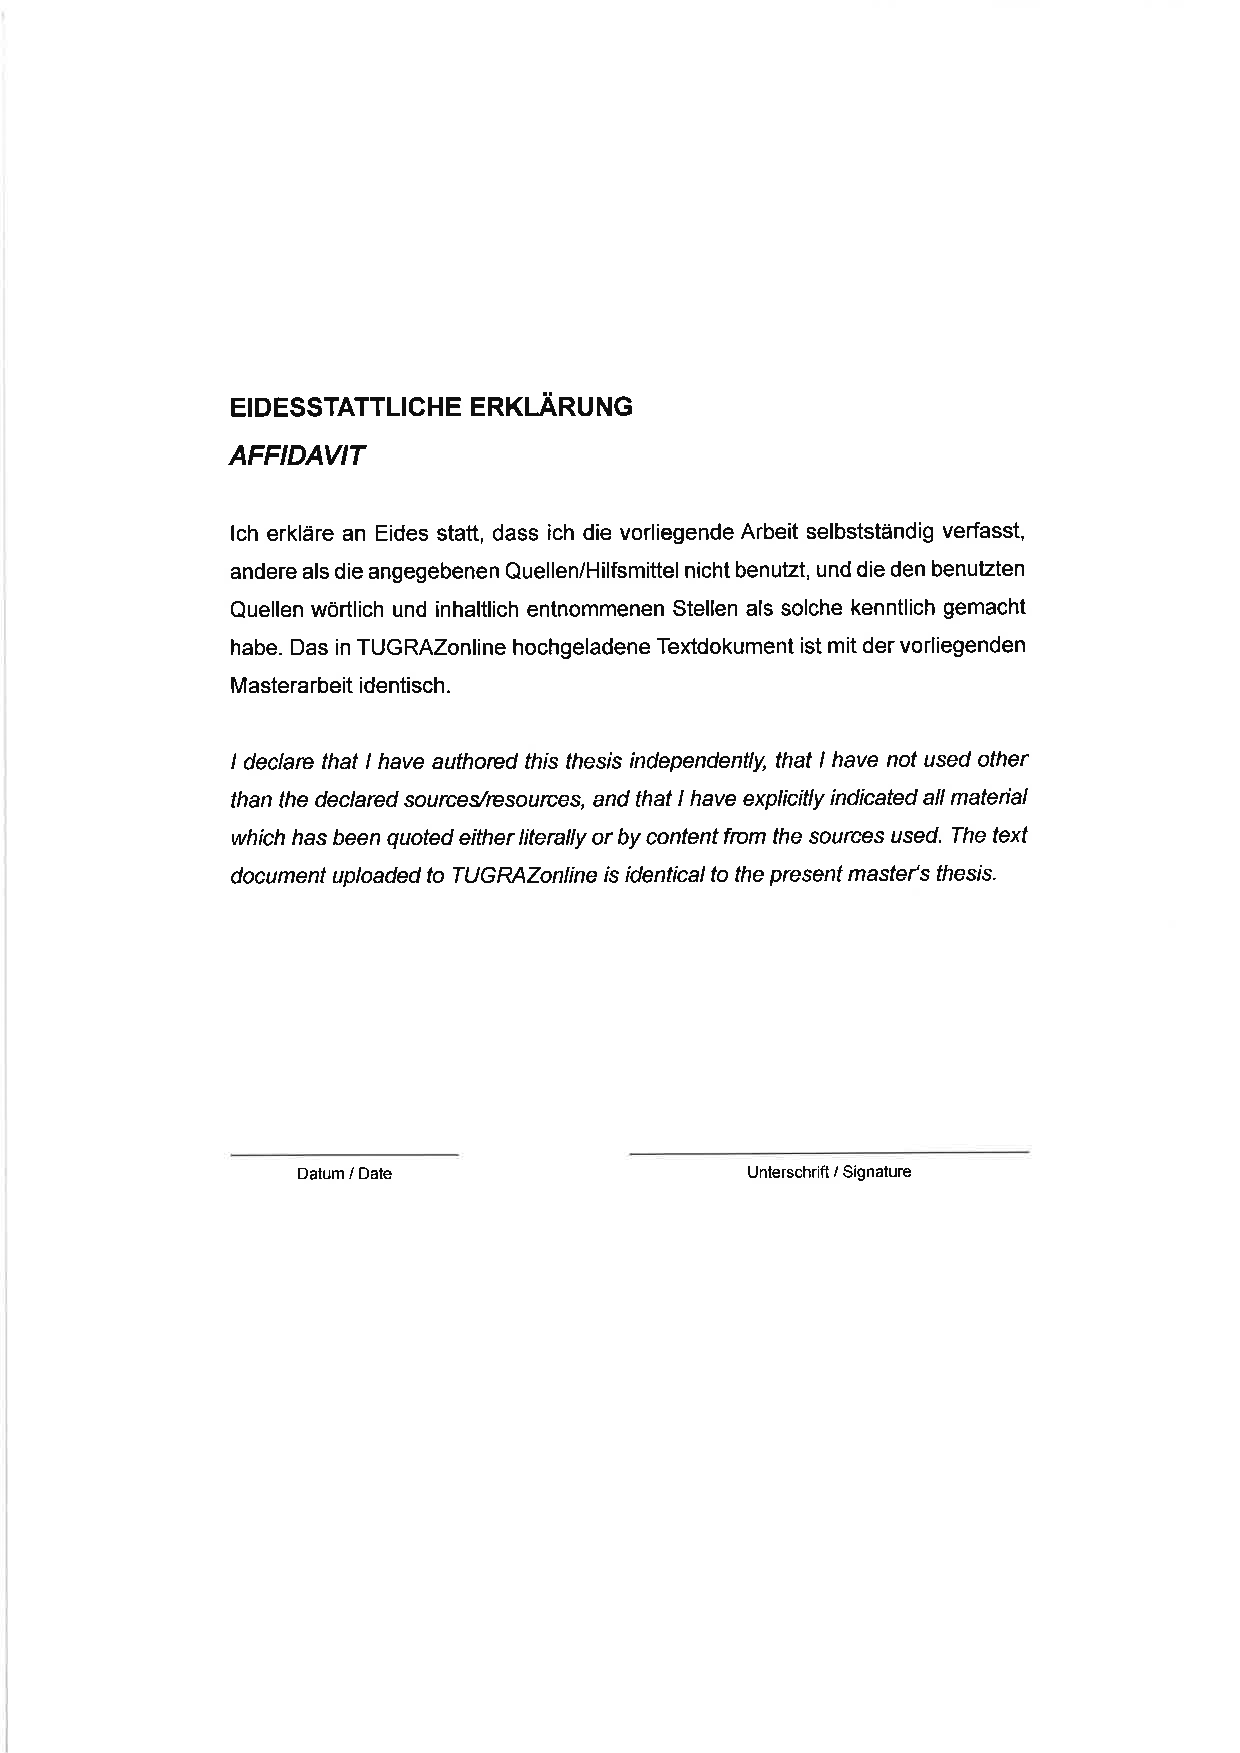
\includepdf[pages={1}]{Eidesstattliche.pdf}

\tableofcontents

\mainmatter
\chapter{Introduction}
%\pagenumbering{arabic}
\setcounter{page}{1}
In the course of this thesis two different dopants were investigated spectroscopically on and in helium nanodroplets. The helium nanodroplet method is a well established technique to isolate dopants and cool them to temperatures of about $\unit[0.37]{K}$. Helium has several properties that make the element unique for spectroscopic investigations: It is transparent from the ultra-violet up to the infrared spectral range, it is superfluid below $\unit[2.18]{K}$ (at normal pressure) and interactions between helium and dopants are weak. \\
Spectroscopy with the helium nanodroplet technique has been used at our institute for several years and has lead to new and interesting insights into different species. %The first experiments were done with alkali atoms such as Rb, because of their simple electronic configurations (only one valence electron). The next step was the investigation of alkaline earth metals, like Ca and Sr, with two valence electrons.
Recently our group started to investigate alkali-alkaline earth molecules such as LiCa \cite{krois-lica}. At the beginning of this thesis ongoing research was dedicated to the investigation of the RbSr molecule. The results, obtained with REMPI-TOF and LIF spectroscopy, are summarized in chapter \ref{chap:rbsrresults} and described in more detail in the PhD thesis of G\"unter Krois \cite{krois-doc}. The theoretical calculations for the RbSr molecule were done by Johann Pototschnig.

In addition, spectra for gold in helium nanodroplets were obtained with REMPI-TOF spectroscopy. The gold spectra were recorded in a different laboratory and with a different laser system than the RbSr experiments. The differences and similarities between the two experiments are described in chapter \ref{chap:auex}. To reach sufficiently high vapor pressures for gold, a high temperature pick up source was installed. Furthermore, a LabView PID temperature controller was programmed. The pick up source and the LabView program are described in chapters \ref{chap:goldoven} and \ref{chap:tempprogram}, respectively. The obtained gold spectra are discussed in chapter \ref{chap:aurempi}.

\chapter{Theoretical Background}
This chapter covers the theoretical background needed to understand the experimental results given in chapter \ref{chap:results}. In the following the properties of helium, the supersonic gas expansion, cluster formation and the fundamentals of the pick up process are explained in detail. At the end of this chapter the basics of atomic and molecular denotations are briefly summed up.
More informations on a given topic can be found in the literature referenced in the respective sections.


\section{Helium}
\vspace{-0.5\baselineskip}
Helium plays an important role in our experiments. It occurs in form of two stable isotopes: $^4$He and $^3$He with a natural abundance of $99.999863 \%$ and $0.000137 \%$, respectively \cite{crc}. Therefore the term "helium" in this thesis refers to $^4$He if not stated otherwise. High purity helium is used as a cold matrix to isolate the species, which we analyze. Advantages of helium are for example its transparency for light from the infrared up to the ultraviolet spectral regime or the fact that interactions with species are very weak (least perturbing matrix). In the following an overview of the physical properties of helium is given.

\subsection{Zero point energy}
\vspace{-1\baselineskip}
It is not possible to solidify helium at normal pressure. It stays liquid starting from the boiling point at $\unit[4.2]{K}$ down to absolute zero temperature. Pressures as high as $\unit[25]{bar}$ are needed to reach the solid phase which explains why it was not observed for a long time. This behavior can be explained via comparing the zero point energies of liquid and solid helium. The zero point energy is the energy difference between a quantum system in its ground state and the energy the system would have classically at its minimum. It follows from the Heisenberg uncertainty principle (equation \ref{uncertainty-principle}) that the ground state energy of a quantum system is greater than zero, where in contrast, the lowest possible energy of a classical system equals zero.

\begin{align}  \label{uncertainty-principle}
\Delta x \cdot \Delta p \ge \frac{\hbar}{2} .
\end{align}

The uncertainty principle states, that two not commuting observables cannot be measured simultaneously with arbitrary accuracy. To fulfill equation \ref{uncertainty-principle} the uncertainties of the position $\Delta x$ and momentum $\Delta p$ of the atoms within the liquid phase have to be nonzero. This also results in potential ($E_{pot} \propto x^2$) and kinetic ($E_{kin} \propto p^2$) energies greater than zero. Therefore the ground state energy, defined as $E_{pot} + E_{kin}$, has to be positive and nonzero as well. \\
It is possible to explain why helium stays liquid under normal pressure via comparing the zero point energies of the liquid and the solid phase. For the solid phase the zero point energy is as high as $\unit[7]{meV}$ which is equivalent to a temperature of $\unit[70]{K}$ \cite{lackner}. The zero point energy of the liquid helium is below this value. Therefore the liquid phase of helium is favored. Because the zero point energy is a quantum effect, liquid helium is also called a quantum liquid. \\
The aggregate state of helium at certain conditions (pressure, temperature) can be determined from the p-T phase diagram shown in figure \ref{he-phase-diagram} \cite{fliessbach}. The diagram shows the ambient pressure in bar over the temperature in Kelvin. Note that the phase diagram shows a fourth (superfluid) state in addition to the three expected aggregate states. At normal pressure superfluidity occurs below a transition temperature of about $T_\lambda = \unit[2.18]{K}$ \cite{toennis} and \cite{ernst2011}.
\begin{figure}[ht]
\centerline{
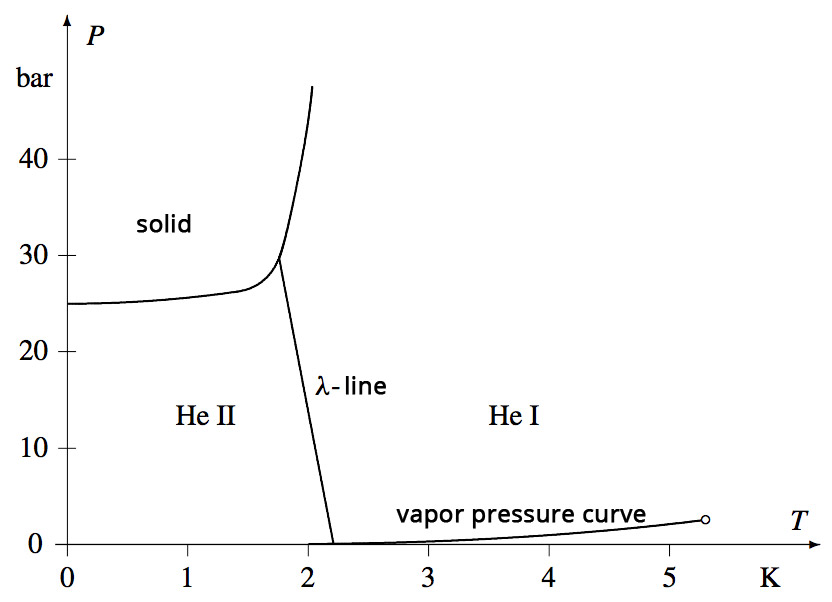
\includegraphics[width=11cm]{./helium/phasediagram.jpg}}
\captionabove{\label{he-phase-diagram} \textsl{Helium p-T phase diagram showing ambient pressure in bar over temperature in K. The critical point can be identified at $\unit[2.2]{bar}$ and $\unit[5.3]{K}$. The superfluid phase can be observed at normal pressure below temperatures of $T_\lambda = \unit[2.18]{K}$. Modified from \cite{fliessbach}. }}
\end{figure} \\
Because the helium matrices used in our experiments are superfluid, a short overview of this intriguing property is given in the following section.

\subsection{Superfluidity}
\vspace{-1\baselineskip}
Superfluidity is a quantum effect and has been observed for $^4$He, $^3$He \cite{only-superfluid}, para-hydrogen \cite{superh} and $^6$Li \cite{superli}. A superfluid state is characterized through unusual properties like a vanishing internal friction, very high heat conductivity and intriguing effects like film flow and the helium fountain. Superfluidity was discovered by Kapitza in 1938 \cite{kapitza}. Some readers may be interested in the historical paper about the discovery \cite{super-story}.

Normal liquid helium is also called helium I whereas superfluid helium is called helium II. Helium I and helium II are separated through the $\lambda$-line which marks a second order phase transition (see figure \ref{he-phase-diagram}). This transition type is characterized by a singularity in its specific heat capacity $c_p$. Interestingly, the transition temperatures of bosonic $^4$He ($T_\lambda = \unit[2.18]{K}$) and fermionic $^3$He ($T_\lambda = \unit[3\cdot10^{-3}]{K}$) are very different \cite{toennis}. This can be understood with the theory of ideal bose gases (IBG) and ideal fermi gases (IFG). The description of properties such as superfluidity or superconductivity is based on a macroscopic wave function. This means a macroscopic amount of particles is describable with the same wave function, which is only possible for bosons. In case of superconductivity, electrons (fermions) pair together to form bosons. A very similar mechanism leads to superfluidity of fermionic $^3$He, requiring a much lower temperature than $^4$He \cite{fliessbach}. Note that this mechanism is not a second order phase transition, thus having other properties than the $^4$He phase transition.

Several theories exist to describe the characteristics of superfluidity. A very good overview is given in \cite{fliessbach}. Two of those theories, the two-fluid model and the quasi particle model, will be discussed in the following.

\subsubsection{The two-fluid model}
\vspace{-1\baselineskip}
The two-fluid model by Tisza \cite{tisza} postulates the liquid helium density as a mixture of a superfluid and a conventional part. Mathematically this can be expressed as

\begin{align}  \label{super-density}
\rho = \rho_s(T) + \rho_n(T) .
\end{align}

In formula \ref{super-density} $\rho_s(T)$ represents the density of the superfluid and $\rho_n(T)$ the density of the normal part of the liquid. Both parts are not separated spatially, but are very different in their physical properties. The ratio between the superfluid and the normal part varies with temperature. At absolute zero the superfluid density $\rho_s$ is one in contrast to the transition temperature where $\rho_s$ is zero \cite{fliessbach}.

\subsubsection{The quasi particle model}
\vspace{-1\baselineskip}
Another approach is the quasi particle model by Landau \cite{landau}. As denoted above, the $\lambda$-transition is tightly bound to the theory of ideal bose gases. The quasi particle model is based on this theory and describes superfluidity with the possible excitations of particle energies $\epsilon$ in an ideal bose gas. The excitations are represented by quasi particles, giving the model its name. Experimentally the elementary excitations are for example observable through inelastic neutron scattering. In that way one can obtain the dispersion relation giving the particle energy $\epsilon$ over the wave vector $k$. The relation is shown in figure \ref{quasi-disp}.

\begin{figure}[ht]
\centerline{
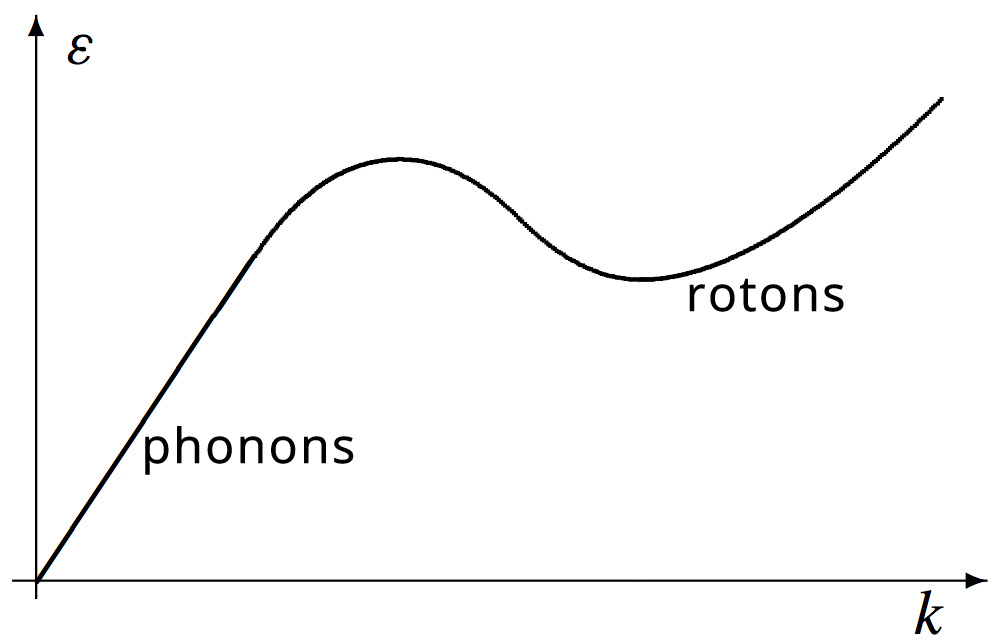
\includegraphics[width=10cm]{./helium/DispRel.jpg}}
\captionabove{\label{quasi-disp} \textsl{The dispersion relation gives the particle energy $\epsilon$ over the wave vector $k$. Phonon and roton contributions characterize the dispersion relation at different wave vectors. Taken from \cite{fliessbach}, modified. }}
\end{figure}

The dispersion relation in figure \ref{quasi-disp} is valid for temperatures $T \lesssim \unit[2]{K}$. For very low temperatures ($T < \unit[1]{K}$) the behavior is determined by the linear part which results mainly from phonon contributions ($c_V \propto c_{phonons}$). In this case the specific heat $c_V$ is proportional to $T^3$. At temperatures above $\unit[1]{K}$ the contribution of rotons dominates ($c_V \propto c_{rotons}$). The name "roton" has developed historically and has no deeper meaning. \\
Within the quasi particle model the specific heat is expressed as the sum $c_V = c_{phonons} + c_{rotons}$. In this way the model quantitatively describes superfluidity via the determination of the specific heat. The model does not describe the $\lambda$-transition itself \cite{fliessbach}.


\section{Formation of helium droplets}
\vspace{-1\baselineskip}
This section discusses the process leading to the formation of helium clusters which are used as matrices. Because these clusters are liquid, they are also referred to as ''droplet''. Beside the advantages mentioned in the helium section the droplets also enable the formation of clusters and molecules not observable otherwise. As a result of those remarkable properties Lehmann and Scoles have termed He$_N$ as the ''ultimate matrix for spectroscopy'' \cite{ultimate}. \\
The helium droplets are build with a method called ''supersonic gas expansion'' which is explained in the next section.

%and build a continuous beam. Each nanodroplet can contain between $100$ and $10^6$ single helium atoms and picks up the desired species for further spectroscopic investigations. In our experiments we form droplets with about $10000$ helium atoms. \\
%Because those droplets are a fundamental part of our experiments the next sections deal with their creation and the doping process. Note that the term ''cluster'' is partially used as a synonym for ''droplet'', which refers to the special case of a liquid cluster.


\subsection{The supersonic gas expansion}
\vspace{-1\baselineskip}
The phase diagram in figure \ref{he-phase-diagram} shows that very low temperatures are necessary to condensate helium and form droplets. Condensation sets in when the cooling path crosses the vapor pressure curve. This is called sub critical expansion. The supersonic gas expansion is an adiabatic expansion through a nozzle with high cooling rates and particle velocities higher than the local velocity of sound (figure \ref{supersonic}). The sizes of the droplets follow a logarithmic normal distribution and their velocities lie within a very narrow distribution ($\frac{\Delta v}{v} \approx 0.01-0.03$, with the FWHM as $\Delta v$) \cite{scoles} \cite{scoles2}. The beam velocity depends on the stagnation conditions and lies between $200$ and $\unit[400]{m/s}$ \cite{toennis}.\\
To reach the sub critical regime in the phase diagram, the nozzle and the gas are cooled. For gas pressures of about $\unit[60]{bar}$ the temperature has to be lower than $\unit[25]{K}$ in order to form droplets \cite{nanolab}. Temperatures of $\unit[10-16]{K}$ are common in our spectroscopic experiments. Pressure and temperature which characterize the expansion are referred to as ''stagnation conditions''. \\
%The supersonic gas expansion is an adiabatic process described by \ref{isentropic}, a product of temperature and volume \cite{demtr1}. $\gamma$ in the exponent of V is the adiabatic index defined in \ref{}.
% \begin{align}  \label{isentropic}
% T \cdot V^{\gamma -1} = const
% \end{align}
The nozzle typically has a diameter of about $\unit[5]{\mu m}$. Gaseous and very pure helium is forced to expand under high pressures into the first vacuum chamber of the apparatus. Common settings are a helium pressure of $\unit[60]{bar}$ and a vacuum pressure of about $\unit[10^{-4}]{mbar}$ in the source chamber. Figure \ref{supersonic} shows the process with different velocity regimes in units of M, the Mach number. As denoted in the graphic, the beam reaches the local velocity of sound at the exit of the nozzle (M=1). This is only valid if the ratio between the pressures $p_0$ and $p_a$ fulfills equation \ref{pressure-condition} (with $p_a$ the background pressure in the source chamber and $p_0$ the stagnation pressure). In this case the pressure at the nozzle exit becomes independent of $p_a$.

\begin{align}  \label{pressure-condition}
\frac{p_0}{p_a} \geq \left(\frac{\gamma + 1}{2}\right)^{\frac{\gamma}{\gamma - 1}}.
\end{align}

The ratio between $p_0$ and $p_a$ is typically in the order of $10^8$. $\gamma$ is the adiabatic exponent of the gas. It is defined as the ratio of specific heat capacity at constant pressure $c_p$ and the specific heat capacity at constant volume $c_V$. This can also be expressed through the degrees of freedom $f$ of gas particles. For helium, equation \ref{adiabatic-exponent} gives $\gamma = 5/3$.

\begin{align}  \label{adiabatic-exponent}
\gamma = \frac{c_p}{c_V} = \frac{f+2}{f}
\end{align}

The zone between nozzle and mach disk is called zone of silence. The zone marks the regime between two points where the beam velocity equals the local velocity of sound.

\begin{figure}[ht]
\centerline{
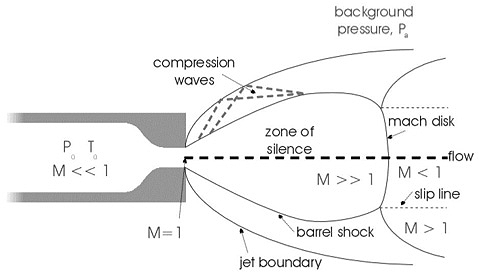
\includegraphics[width=13cm]{./expansion/supersonic-expansion_sharp.jpg}}
\captionabove{\label{supersonic} \textsl{Supersonic gas expansion with different velocity regimes expressed in units of M, the Mach number \cite{nagl}. The zone of silence marks the regime from the nozzle to the Mach disk.}}
\end{figure}

\begin{align}  \label{local-sound-velocity}
a(z) = \sqrt{\gamma \frac{p(z)}{\rho(z)}}
\end{align}

The local velocity of sound is calculated with formula \ref{local-sound-velocity} taken from \cite{scoles}. $p(z)$ and $\rho(z)$ are the pressure and the gas density, respectively. Both depend on the distance $z$ measured from the nozzle exit.

In case of a supersonic expansion, fulfilling condition \ref{pressure-condition}, the beam expands along the thin, dashed lines in figure \ref{supersonic}, exceeding the velocity of sound ($M > 1$) at the outer regions of the beam. A higher velocity also means a lower pressure. In fact the pressure drops under $p_a$. This causes shock waves (barrel shock), which focus the beam spatially but in turn reduce its velocity to $M < 1$ (inner part of the beam, thin dashed lines). The shock waves travel in beam direction and are separated from regions with $M < 1$ through the Mach disk where $M = 1$. The position of this disk can be calculated with the diameter $d$ of the nozzle via equation \ref{mach-dist} from \cite{pauly}.

\begin{align}  \label{mach-dist}
z_M = 0.67d\sqrt{\frac{p_0}{p_a}}.
\end{align}

The distance $z_M$ is measured from the nozzle exit. With the common stagnation conditions ($p_0 = \unit[60]{bar}, p_a = \unit[6\cdot10^{-4}]{mbar}$ and $d = \unit[5]{\mu m}$) the zone of silence is approximately $\unit[3.7]{cm}$ long \cite{skimmer-pos}.

\begin{figure}[ht]
\centerline{
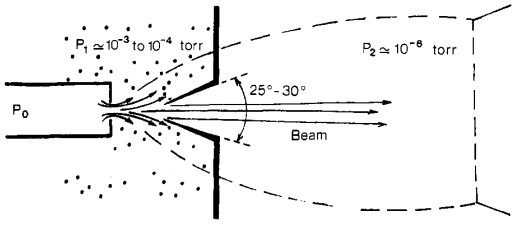
\includegraphics[width=13cm]{./expansion/with-skimmer.jpg}}
\captionabove{\label{exp-with-skimmer} \textsl{Illustration of the beam extraction with a skimmer. The dashed region is the zone of silence \cite{skimmer-pos}. }}
\end{figure}

During the expansion the gas cools down with very high cooling rates of about $\unit[10^{11}]{K/s}$ \cite{stein}. These cooling rates in combination with a pre cooled nozzle enable the condensation of gaseous helium and the formation of droplets. A narrow orifice called skimmer ($\unit[400]{\mu m}$ diameter) extracts the beam. The ideal position for the skimmer depends on the stagnation conditions and can be calculated with

\begin{align}  \label{skimmer-position}
z_S = 0.125d\left(\frac{d}{\lambda_0}\frac{p_0}{p_a}\right)^{1/3}.
\end{align}

$z_S$ is the position of the skimmer and lies within the zone of silence. $\lambda_0$ is the mean free path of the particles. A qualitative illustration of the skimmer position is given in figure \ref{exp-with-skimmer} from \cite{skimmer-pos}. Note that the dashed line marks the zone of silence.

After dealing with droplet formation and extraction the following section will provide details about the size distribution of helium droplets.


\subsubsection{Droplet temperature and size distribution}
\vspace{-1\baselineskip}
During a supersonic gas expansion cooling is caused by particle collisions. After about $1000$ nozzle diameters ($\unit[5]{mm}$ for a $\unit[5]{\mu m}$ orifice) collisions between helium atoms get very rare and the beam consists of helium droplets and single atoms. The droplets within the beam do not grow anymore through condensation, but cooling still takes place due to evaporation of helium atoms. This process cools the droplet to a very stable final temperature of $\unit[0.37]{K}$ (figure \ref{cluster-formation}).
\begin{figure}[ht]
\centerline{
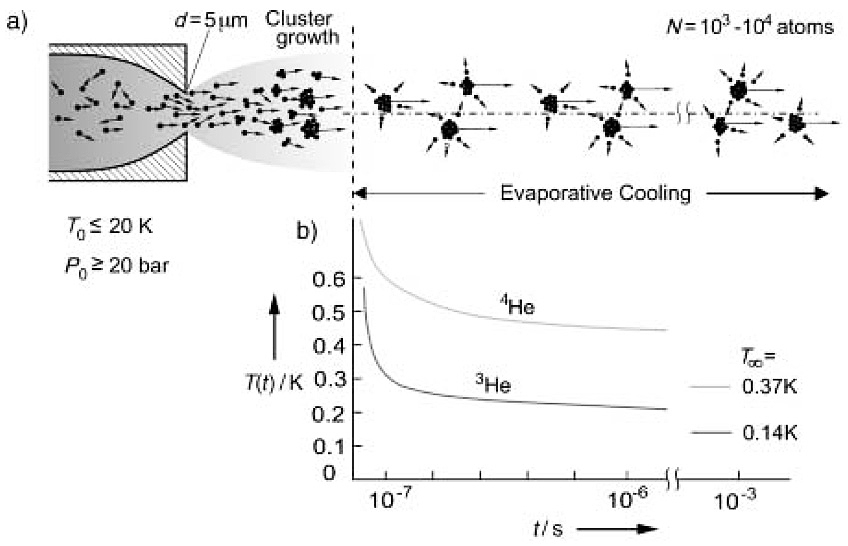
\includegraphics[width=12cm]{./expansion/cluster-formation_sharp.jpg}}
\captionabove{\label{cluster-formation} \textsl{a) Cluster formation within a distance of about $1000$ nozzle diameters ($\unit[5]{mm}$). b) Clusters are cooled further through evaporation of helium atoms. The exponential decay of the temperature over time is shown in the diagram. Note that the final temperatures for $^3He$ and $^4He$ are different. \cite{toennis} }}
\end{figure}\\
The droplet temperature was first determined by Hartmann, Miller, Toennis and Vilesov \cite{he-tempNew}. They calculated the temperature from the rotational infrared spectrum of the $SF_6$ molecule inside a helium droplet. Because the occupation of rotational levels follows a Boltzmann distribution, which is temperature dependent, they were able to determine the temperature from this spectrum. The calculations gave a droplet temperature of $\unit[0.37]{K}$, definitely in the superfluid regime of the p-T phase diagram shown in figure \ref{he-phase-diagram}. The high specific heat, which comes with superfluidity, and evaporation cooling are the reasons why this temperature is so stable during experiments. Because the helium droplets are transparent for infrared and ultraviolet light it is not possible to heat them noteworthy with lasers used in our experiments \cite{laser-heating}.

The cluster size distribution is a logarithmic normal distribution and can be calculated with formula \ref{lognormalformula} taken from \cite{speed-distr}. With typical stagnation conditions ($p_0 = \unit[60]{bar}$, $T_{nozzle} = \unit[15]{K}$) the distribution has its maximum at about $10^4$ atoms per cluster. In the formula the average cluster size $\bar{N}$ can be used for the mean value $\mu$ and the standard deviation $\sigma$ can be calculated from the half width $\Delta N_{1/2}$ (see \cite{speed-distr}). Note that $\bar{N}$ and $\Delta N_{1/2}$ are comparable in value as table \ref{cluster-values} shows.
\begin{align}  \label{lognormalformula}
p_N(N) = \frac{1}{\sqrt{2\pi}N \sigma} exp\left(- \frac{(lnN - \mu)^2}{2\sigma^2}\right)
\end{align}
Figure \ref{log-dist} taken from ref. \cite{loga-distributions} shows different distributions for different temperatures. These distributions were obtained by deflection experiments with a helium pressure of $\unit[80]{bar}$. The figure shows that the maximum of a distribution shifts to larger cluster sizes at lower temperatures. Distributions with a maximum at lower cluster sizes show a narrower distribution compared to ones of larger cluster sizes (at lower temperatures).

\begin{figure}[ht]
\centerline{
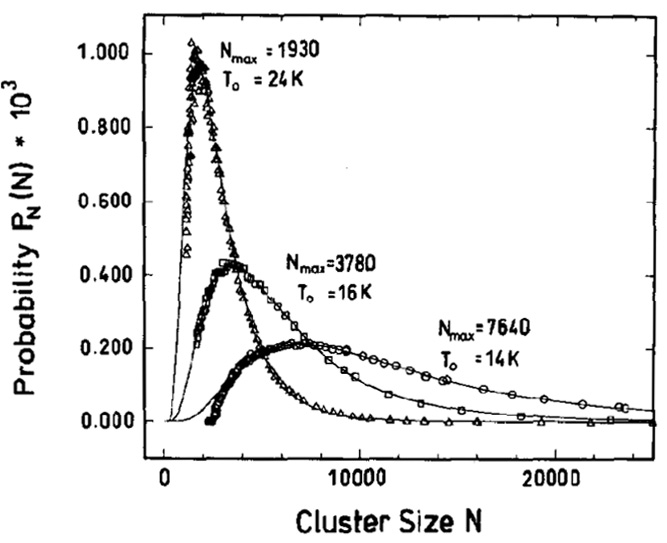
\includegraphics[width=11cm]{./expansion/log-normal-distribution.jpg}}
\captionabove{\label{log-dist} \textsl{Helium cluster size distribution for $p_a = \unit[80]{bar}$ and different temperatures \cite{loga-distributions}. }}
\end{figure}

\begin{table}[h]
%\centering
\captionabove{\textsl{Typical values for the mean value and the half width of cluster size distributions at different temperatures. \cite{loga-distributions} }}
\label{cluster-values}
\begin{center}
% use packages: array
\begin{tabular}{c|c|c}

 T [K] & $\bar{N}$ & $\Delta N_{1/2}$ \\

\hline
\rowcolor{hellgrau}
24 & 3170 & 2670 \\
\rowcolor{dunkelgrau}
16 & 7220 & 7870  \\
\rowcolor{hellgrau}
14 & 14400 & 15700  \\
\end{tabular}
\end{center}
\end{table}

The previous sections were dedicated to helium and the formation of droplets. The next important step in our experiments is the pick up process where the helium droplets are doped with the desired species. This pick up process is described in the following section.

\subsection{Doping helium clusters}
\vspace{-1\baselineskip}
Doping describes the process where impurities, in our case the spectroscopically relevant elements, are picked up by the droplet. The pick up takes place in so called ''pick up cells''. Once the helium droplets enter the cells they collide statistically with gaseous dopants. The probability for a collision increases with the vapor pressure of the dopant. Vapor pressures of about $\unit[10^{-4}]{mbar}$ are sufficient for the pick up process in our experiments. In case of solid species the pressure is controlled via the temperature used to evaporate the dopant. For gaseous species the cell is a cylinder with a gas inlet.

The pick up process follows the Poisson statistics which is defined by

\begin{align}  \label{poisson}
P(n|\lambda) = \exp(-\lambda) \frac{\lambda^n}{n!}.
\end{align}

Formula \ref{poisson} gives the probability to pick up n atoms. $\lambda$ is the expectation value of pick up processes ( ref. \cite{vdl}) which is correlated to the droplet size (geometrical cross section), the length of the pick up cell and the vapor pressure of the dopant.

Once an atom is picked up it is located within the helium cluster or on its surface \cite{pickup-desc}. If a second atom is picked up, their long reaching van der Waals forces cause attraction between them and dimerization follows. This process is repeated for every subsequently added atom which leads to the formation of clusters of the species. This process takes place in very short time scales of $\unit[10^{-8} - 10^{-10}]{s}$ \cite{toennis}. During the formation, binding energy is set free and causes evaporation of helium atoms. After the molecule is formed and stabilized, helium evaporation cools the system to $\unit[0.37]{K}$. In this way the helium droplet works as a personal nanosized cryostat for foreign atoms or molecules. \cite{evap-cryo} and \cite{ernst2011}

\begin{figure}[ht]
\centerline{
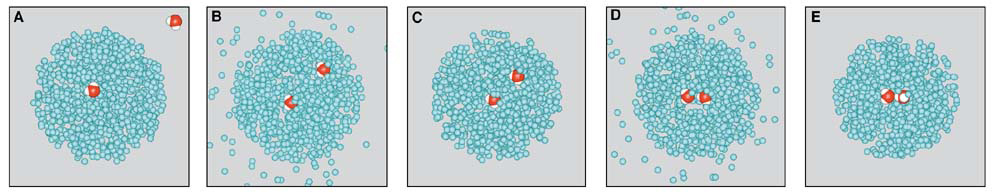
\includegraphics[width=13cm]{./doping/doping-helium.jpg}}
\captionabove{\label{doping-helium} \textsl{The schematic pick up process and dimerization within a helium cluster. Evaporation caused by a pick up process (B) and due to dimerization (D).\cite{cool}  }}
\end{figure}

Whether a molecule tends to stay on the surface or to immerse into the droplet can be estimated by the dimensionless Ancilotto parameter $\lambda$ \cite{ancil-param}. It is defined as the ratio between the free energy gain and the free energy cost of forming a cluster inside the helium droplet. The free energy gain is mainly determined by the depth of the pair potential between the dopants and the helium atoms. The free energy cost is proportional to the surface tension of helium. In this way the parameter gives a relative measure of the energy gain associated with the immersed state \cite{ancil-param}. For this estimation an infinite impurity mass and a Lennard-Jones pair potential between helium and species are assumed. The formula for the Ancilotto parameter is given in \ref{ancilotto}.

\begin{align}  \label{ancilotto}
\lambda = \frac{\rho \epsilon r_{min}}{\sigma 2^{\frac{1}{6}}}
\end{align}

$\rho$ is the number density of helium, $\epsilon$ and $r_{min}$ are the depth and equilibrium distance of the Lennard-Jones potential well. $\sigma$ stands for the surface tension of helium. The constant factor $2^{\frac{1}{6}}$ is related to the Lennard-Jones potential.
Small values of $\lambda$ mean that immersion is not favorable. A value of about $\lambda = 1.9$ separates the atoms which stay on the surface from those which immerse \cite{acil-param-value}. The Ancilotto parameter for Rb is $0.79$ (ref. \cite{ancil-param}) which indicates that the atom stays on the surface of the droplet. Gold has an Ancilotto parameter of $6.42$ (ref. \cite{tong}) indicating that the atom immerses.

After describing the theoretical basics of helium droplets and the doping process it is now appropriate to deal with spectroscopy.

\section{Spectroscopy}
\vspace{-0.5\baselineskip}
This section covers the theoretical background for our spectroscopic investigations. It informs about discrete energy levels in atoms and molecules and gives an overview of the spectroscopic annotations used in chapter \ref{chap:results} of this thesis. Due to reasons of simplicity this section will begin with atoms. One and multi electron systems are covered separately for single atoms as well as for the next section about molecules.

\subsection{Atoms}
\vspace{-1\baselineskip}
In case of atoms every state can be characterized with four quantum numbers n, l, s and j. This is only true if no electric or magnetic fields are applied. For all further considerations external fields are neglected \cite{demtr3}. \\
If quantum numbers are written in lower case letters they describe the state of a single electron whereas quantum numbers in capital letters (L, S, J) describe atomic states.
From all atoms the hydrogen atom is the most simple to describe. It has only one valence electron and can be described without electron-electron interactions within a model where energy levels only depend on the principal quantum number n. The different energies are then calculated via formula \ref{en}. This is equivalent to the Bohr atomic model \cite{vdl-fqm}.

\begin{align}  \label{en}
E_n = - \frac{m e^4}{2 \hbar^2} \frac{Z^2}{n^2} \hspace{2 cm} n = 1,2,3,...
\end{align}

All four quantum numbers n, l, s and j obey several rules. For a given principal quantum number n, only orbital angular momentum quantum numbers $l < n$ are allowed. For every $E_n$ there are $l=0,1,2,...,n-1$ possibilities for the orbital angular momentum quantum number. Energy levels with a specific l value are denoted with the letters s ($l=0$), p ($l=1$), d ($l=2$), f ($l=3$),... For hydrogen, energy levels with the same n but different l are degenerated, which means that they have the same energy.

To explain the two remaining quantum numbers s and j the electron spin $s= \frac{1}{2}$ has to be taken into account. The electron spin is a quantum mechanical property of an electron and has all characteristics of a classical momentum except that it is not caused by rotation. The sum of electron spin $s$ and orbital angular momentum $l$ results in the total angular momentum $j = l + s$. In that way the state of the single electron and therefore of the hydrogen atom is characterized.

\subsubsection{Multiplicity and coupling schemes for atoms with one or more valence electrons}
\vspace{-1\baselineskip}
For the general case of one or more electrons $L, S$ and $J$ are introduced and describe the whole atom, not only a single electron. The total spin $S$ for an atom with only one valence electron equals the spin of the single electron $S = \frac{1}{2}$. The different possible orientations of $S$ with respect to $L$ leads to energy splitting of a single level into two states with slightly different energies (for atoms with $L > 0$). To quantify the splitting of energy levels the multiplicity, defined as $2S + 1$, is introduced. For a system with a single electron the multiplicity is two. This reflects the fact that an electron has two possible spin orientations in the electric field caused by its orbit, namely $s = +\frac{1}{2}$ or $s = -\frac{1}{2}$. \\
In case of a single electron the total angular momentum $J$ is calculated as $J = |L \pm S|$. For atoms with more than one valence electron the total angular momentum $J$ is determined in two different ways, depending on whether the energy levels are dominated by electron-electron interactions or spin-orbit interactions. Which interaction dominates mainly depends on the atomic number of the atom and therefore on the charge of the nucleus. For atoms with $Z \gtrsim 40$ the spin-orbit interactions are dominant. In this case the spin of each electron $s_i$ couples with its orbital angular momentum $l_i$. Every electron has a total angular momentum $j_i = l_i + s_i$. The total angular momentum of the atom is then $J = \sum\limits_{i} j_i$. This is known as jj-coupling.

In contrast, light atoms are better described by $\mathbf{LS}$-coupling. Low atomic numbers mean weak spin-orbit interactions. The electron-electron interactions dominate. As a consequence the electrons disturb each other in a way that $l_i$ and $s_i$ do not couple to $j_i$ anymore. In fact all $l_i$ and all $s_i$ couple separately to form $L = \sum\limits_{i} l_i$ and $S = \sum\limits_{i} s_i$ respectively. $L$ and $S$ then couple to $J = L + S$.

For those multi electron systems the multiplicity can be higher than two, depending on number and spin alignment of the electrons. States with multiplicity three or four are called triplet or quartet states, respectively. States with multiplicity one ($S = 1$) are called singlet states.


\subsubsection{Spectroscopic denotation of energy states}
\vspace{-1\baselineskip}
Every atomic state is denoted with the four already familiar quantum numbers (n, L, S, J) according to the scheme in \ref{general-atomic-energy-level}.

\begin{align}  \label{general-atomic-energy-level}
n ~ ^{2S+1}L_J
\end{align}

As a simple example an excited state of helium is given. Helium is a very light atom and can therefore be described by $\mathbf{LS}$-coupling.

\begin{align}  \label{atomic-energy-level}
2 ~ ^3P_2
\end{align}

The excited electron has the principal quantum number $n = 2$. The elevated 3 means that it is a triplet state which can only result from a total spin $S = 1$. There are three possibilities to reach a total spin of one with only two electrons: Both electrons spin-up, both spin-down and one electron up and the other down. Figure \ref{simple-triplet} shows these possibilities graphically.

\begin{figure}[ht]
\centerline{
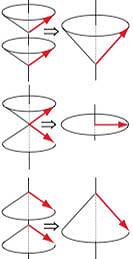
\includegraphics[width=2.5cm]{./spectroscopy/simple-triplet_sharp.jpg}}
\captionabove{\label{simple-triplet} \textsl{The three possibilities to reach $S = 1$ with two electrons. The resulting spin vectors are different in direction but have the same value. Modified from \cite{hertel2008}.  }}
\end{figure}

This energy splitting is also called fine-structure splitting and is shown graphically for the helium $n > 2$ levels in figure \ref{helium-term}.
%Apart from this denotation the energy states can also be illustrated graphically by a term scheme. A term scheme shows states with different total orbital angular momenta (s,p,d,f,..) horizontally shifted. States drawn higher (vertically) are higher in energy. The term scheme for the excited helium state is shown in figure \ref{helium-term}.

\begin{figure}[ht]
\centerline{
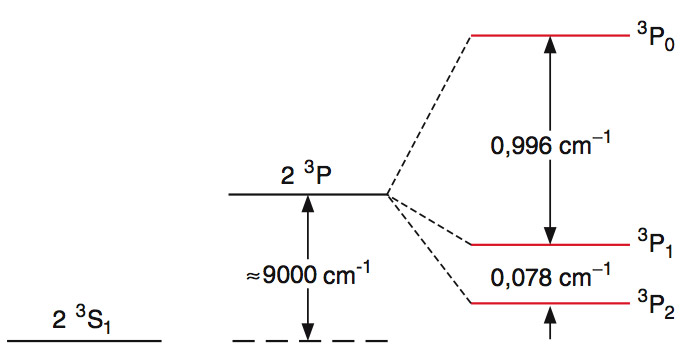
\includegraphics[width=12cm]{./spectroscopy/helium-terms.jpg}}
\captionabove{\label{helium-term} \textsl{Fine structure splitting of the helium $2 ~ ^3P$ level into three states with energy differences stated in $cm^{-1}$. \cite{demtr1}  }}
\end{figure}

The capital letter $P$ in formula \ref{atomic-energy-level} refers to the total orbital angular momentum $L = 1$. The index 2 states, that the total angular momentum $J = 2$. In that way the atomic state is defined.
Transitions between states are possible and obey certain rules. These rules are matter of the next section.

\subsubsection{Selection rules for electronic transitions}
\vspace{-1\baselineskip}
Following from atomic symmetry considerations, electronic transition rules are introduced. In particular three different selection rules must be fulfilled to allow a transition induced by a photon:

\begin{enumerate}
\item $\Delta l = \pm 1$
\item $\Delta j = 0, \pm1$ (except $j=0 \rightarrow j=0$)
\item $\Delta s = 0$
\end{enumerate}

The first rule is equivalent to the conservation of angular momentum (the spin of a photon is 1). The third rule means that multiplicity is also conserved, e.g. forbidding transitions between singlet and triplet systems. \\

In the next section molecular energy levels and their denotations are described.


\subsection{Molecules}
\vspace{-1\baselineskip}
Spectral lines of free atoms are the result of electronic transitions within the atomic shell. Molecules are groups of two or more atoms held together by chemical bonds. The involved atoms can oscillate relatively to each other or rotate around a specific axis. These additional degrees of freedom make rotations and vibrations possible. In that way not only electronic states but also vibrational and rotational states are available in molecules. \\

\subsubsection{The diatomic molecule}
\vspace{-1\baselineskip}
Molecules with two atoms are known as ''diatomic molecules''. The axis leading directly from one nucleus to the other is called the internuclear axis and is defined as the z-axis. Every electronic state in a diatomic molecule is represented by a potential energy curve. Common energy potentials are the Lennard-Jones or the Morse potential. Figure \ref{molpot} shows the Morse potential (Morse) in comparison with the most simplified model, the harmonic oscillator (Parabel). The third energy potential (real) in figure \ref{molpot} is the actual potential for Na$_2$.
The Lennard-Jones and the Morse potential are different mathematical approximations. Especially the Morse potential is often used for modeling diatomic molecules. The harmonic oscillator, as the most simple approach, omits unbound states (it is a parabola with infinite height) and the anharmonic shape of real energy potentials. However it can serve as an approximation for low vibrational states.

\begin{figure}[ht]
\centerline{
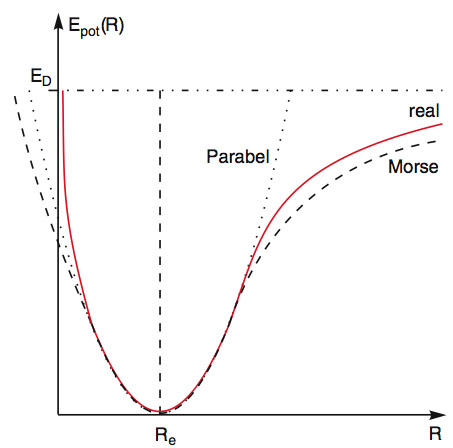
\includegraphics[width=9cm]{./spectroscopy/molecular-potential.jpg}}
\captionabove{\label{molpot} \textsl{Comparison of harmonic, Morse and a real energy potential (Na$_2$). Modified from \cite{demtrodermol} }}
\end{figure}

Various vibrational and rotational states lie within each potential energy curve. Vibrational states are usually denoted with $\nu$, the vibrational quantum number. The energy difference between neighboring vibrational levels decreases with energy. To every vibrational level several rotational levels belong. Figure \ref{vibrotpot} illustrates two different electronic states with vibrational and rotational levels (in the gray rectangles).

\begin{figure}[ht]
\centerline{
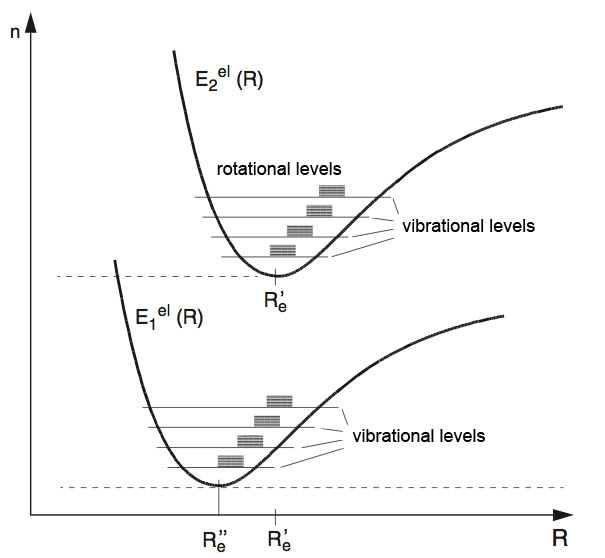
\includegraphics[width=9cm]{./spectroscopy/vib-rot-pot.jpg}}
\captionabove{\label{vibrotpot} \textsl{Two electronic states represented by two molecular potentials energy curves with different equilibrium distances $R'_e$ and $R''_e$. Vibrational and rotational states are drawn within the energy curves. Modified from \cite{demtrodermol} }}
\end{figure}

% The denotation of states for molecules is similar to the notation used for single atoms. Differences between the two notations are described in the following section on the basis of the diatomic molecule \cite{demtrodermol}.

%Our molecular spectroscopy experiments were done with RbSr. For this reason the diatomic molecule is described in the following section leading to the considerations of one and more electron systems and to the molecular denotation.
%In the following the special case of the diatomic molecule is described.

In diatomic molecules the core field of the two nuclei is cylinder symmetric around the z-axis. This causes a precession of the orbital angular momentum vector $\boldsymbol{\ell}$ around the internuclear axis. The vector changes over time and $\boldsymbol{\ell}$ is no longer a conserved quantity. \\
In this section the characteristic quantum numbers for molecules are first introduced for one- and then for multi electron systems. Examples for one electron systems are ions like H$^+_2$ or Li$^+_2$. With these quantum numbers the different coupling schemes and the molecular denotation will be described.


\underline{One electron systems} \\
In the previous section about atoms we differentiated between two coupling schemes (LS- and jj-coupling). For molecules five coupling schemes, called Hund's case (a)-(e), exist. Which Hund's case  describes the molecule best, depends on the dominant interaction. Three interactions have to be taken into account: electrostatic, spin-orbit and rotational interactions.
%In diatomic molecules with only one valence electron the precessing $\boldsymbol{\ell}$ causes a cylindrical magnetic field in z direction in which the spin of the electron aligns (figure \ref{molden}).
For nuclei with low atomic numbers the interactions between $\boldsymbol{\ell}$ and $\mathbf{s}$ are weak. This is described by Hund's case (a). In this case both vectors precess independently around the z-axis. As conserved quantities the two quantum numbers $\lambda$ and $\sigma$ are introduced as projections of $\boldsymbol{\ell}$ and $\mathbf{s}$ onto the z-axis. Their values are $\lambda \hbar$ and $\sigma \hbar$. Figure \ref{molden} illustrates Hund's case (a) for a molecule with one valence electron.

\begin{figure}[ht]
\centerline{
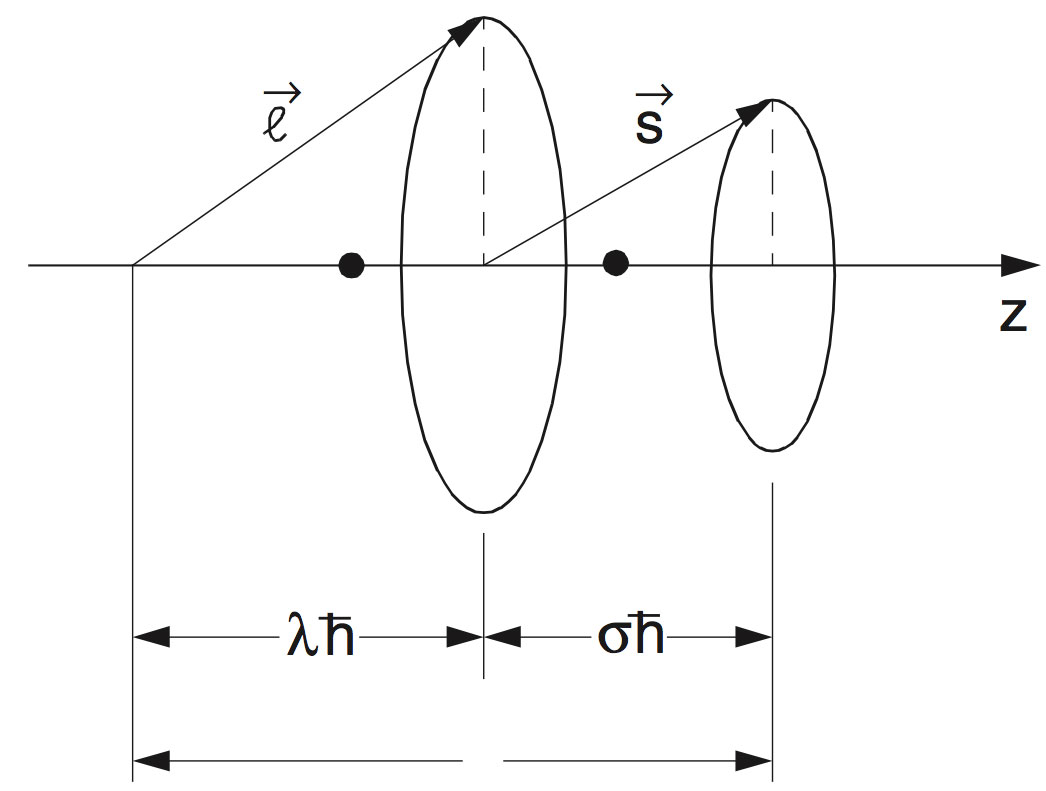
\includegraphics[width=8cm]{./spectroscopy/ls-mol.jpg}}
\captionabove{\label{molden} \textsl{Hund's case (a) for a molecule with one valence electron. $\boldsymbol{\ell}$ and $\mathbf{s}$ are independently precessing. The values of their projections are drawn. From \cite{demtrodermol} }}
\end{figure}

\underline{Two and more electron systems} \\
%For The precessing vectors $\mathbf{L}$ and $\mathbf{S}$ are not ''good quantum numbers'' for molecules, which means they do not describe the molecular states very well. As a consequence the $\mathbf{LS}$-coupling model, known from the atoms section, is not suitable anymore. The different coupling possibilities for molecules are therefore described by Hund's coupling cases. The five idealized cases, $(a)...(e)$, explain coupling via comparing the strength of electrostatic and spin-orbit interactions. For our experiments Hund's case $(a)$ (strong electrostatic, intermediate spin-orbit interaction) and Hund's case $(c)$ (strong spin-orbit interaction) are the most common ones. Both cases are described below. Strong interactions between $\mathbf{L}$ and $\mathbf{S}$ are denoted here as $\mathbf{L-S}$ coupling (note the difference to the atomic $\mathbf{LS}$-coupling model).
For multi electron systems the angular momenta of the electrons couple. In which way they add up is determined by the dominant interactions and therefore again describable by the Hund's cases. The two Hund's cases (a) and (c), which are relevant for this work, are described. Hund's case (a) is characterized by strong electrostatic interactions whereas strong spin-orbit interactions are described by Hund's case (c). Both cases are illustrated for multi electron systems in figure \ref{omega-both}.

\begin{figure}[ht]
\centerline{
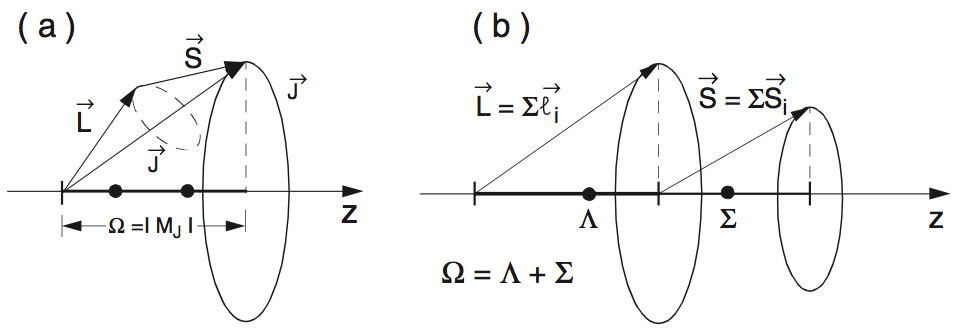
\includegraphics[width=14cm]{./spectroscopy/omega-molecule.jpg}}
\captionabove{\label{omega-both} a) Hund's case $(c)$ strong $\mathbf{L-S}$ interactions. b) Hund's case $(a)$: Independently precessing vectors where the core-field breaks the coupling of $\mathbf{L}$ and $\mathbf{S}$. From \cite{demtrodermol} }
\end{figure}

Figure \ref{omega-both} a) shows the coupling of total orbital angular momentum $\boldsymbol{L}$ and total spin $\boldsymbol{S}$ in case of strong spin-orbit interactions. Because both vectors are precessing, the total angular momentum $\boldsymbol{J} = \boldsymbol{L} + \boldsymbol{S}$ precesses around the internuclear axis. However, to define a quantum number for the total angular momentum vector, $\Omega$ is introduced as the projection of $\boldsymbol{J}$ onto the z-axis. Its absolute value is called M$_J$.

\begin{align}  \label{total-omega}
\Omega = |M_J|, \quad \quad \quad \Omega = J, J - 1,...,\frac{1}{2} \quad or \quad 0
\end{align}

%For molecules with more than one valence electron the orbital angular momenta of the single electrons add up. This is best explained on the basis of the already familiar case of a single atom. For this model both nuclei of the molecule are united to one nucleus with an atomic number calculated as the sum of the two separated nuclei ($Z = Z_A + Z_B$). In terms of $\mathbf{LS}$-coupling the total orbital angular momentum is calculated as sum over all individual angular momenta $\mathbf{L} = \sum\limits_{i} l_i$. The same is valid for the total spin $\mathbf{S}$ of the system $\mathbf{S} = \sum\limits_{i} s_i$. The total angular momentum then is $\mathbf{J} = \mathbf{L} + \mathbf{S}$. Because the electrons are bound within a spherical core-field (one nucleus) the total angular momentum $\mathbf{J}$ does not change over time.
%This simple atomic model is now changed to describe Hund's case $(c)$ of a diatomic molecule. For this, the two united nuclei are separated until they reach their equilibrium distance $r_{min}$. This changes the core-field from a spherical field to an axial-symmetric field. The total angular momentum $\mathbf{J}$ is not time-independent anymore. Only the arithmetic mean within a time period is observable, not $\mathbf{J}$ itself. This value is defined as $M_J$ and it is the projection of $\mathbf{J}$ onto the z-axis. For molecular denotations in case of strong $\mathbf{L-S}$ coupling (Hund's case $(c)$) the quantum number $\Omega$ is introduced as
%\underline{Hund's case (a)} \\
%$\mathbf{L}$ and $\mathbf{S}$ of molecules with low atomic numbers precess independently, because the axial-symmetric core-field prevents the coupling of those vectors. Two projections named $\Lambda$ (z projection of $\mathbf{L}$) and $\Sigma$ (z projection of $\mathbf{S}$) are introduced for this case. Note that this notation is in analogy to the convention for single atoms, with the difference that for molecules greek capital letters are used. In the same analogy states with $\Lambda = 0, 1,2,...$ are denoted as $\Sigma-, \Pi-$ and $\Delta-$states (compare to S,P,D). The total angular momentum Omega for independently precessing $\mathbf{L}$ and $\mathbf{S}$ vectors (weak spin-orbit interaction, Hund's case a) in molecules with more than one electron is defined as
The second case shown in figure \ref{omega-both} b) illustrates the coupling for strong electrostatic interactions, Hund's case (a). The two vectors $\boldsymbol{L}$ and $\boldsymbol{S}$ couple separately to the internuclear axis and precess independently. The orbital angular momenta of the single electrons sum up to form $\mathbf{L} = \sum\limits_{i} l_i$. The same is true for the spins of the electrons forming $\mathbf{S} = \sum\limits_{i} s_i$. Both vectors precess around the z-axis. In this case the two quantum numbers $\Lambda = |M_L|,\quad \Lambda = 0, 1, 2,...L$ and $\Sigma = M_S = s, s-2,...,-s$ are introduced as projections of $\boldsymbol{L}$ and $\boldsymbol{S}$ respectively. For Hund's case (a) $\Omega$ is defined as the sum of $\Lambda$ and $\Sigma$:

\begin{align}  \label{omega-ls}
\Omega = |\Lambda + \Sigma|
\end{align}\\


\underline{Molecular denotations} \\
%In terms of molecular spectroscopy it is common to denote states with capital letters. Those replace the principle quantum number n known from the denotation of single atoms. The molecular ground state is notated with X. The next higher, optically reachable states are denoted with A, B, C,... and so forth, beginning with the energetically lowest state. States that are not reachable optically are denoted with lower case letters a, b, c,...
%With the total spin $S$ and the two projections $\Lambda = |M_J|$ and $\Omega = |\Lambda + \Sigma|$ (Hund's case (a) ) a molecular state is written as
The notation of an electronic state of a diatomic molecule is written with the total spin S, and the two projections $\Lambda = |M_L|$ and $\Omega = |\Lambda + \Sigma|$ as

\begin{align}  \label{mole-denotation}
X^{2S+1}\Lambda_{\Omega}
\end{align}

Note that the capital letter (X) replaced the principal quantum number n known from the atom section. The molecular denotation uses capital letters (A,B,C,...) to notate states reachable from the ground state by electric dipole transitions. States not reachable are denoted with lower case letters (a,b,c,...). The ground state is denoted with X.

The selection rules for electric dipole transitions in molecules are:

\begin{enumerate}
\item $\Delta \Lambda = 0, \pm 1$
\item $\Delta \Omega = 0, \pm1$
\item $\Delta S = 0$
\end{enumerate}



\chapter{Experimental Setup}
\label{chap:expsetup}
This chapter describes the experimental setup of the apparatus in Cluster Lab I, used for the RbSr experiments. A thorough discussion of this setup is given in ref. \cite{nagl}. The setup of the apparatus in Cluster Lab III, used for the gold experiments, is described in chapters \ref{chap:results} and \ref{chap:goldoven}.

The apparatus consists of three chambers which are shown in figure \ref{apparatus-scheme}.


% \begin{itemize}
% \item The source chamber where the molecular beam is created.
% \vspace{-0.5\baselineskip}
% \item The pick up chamber where the helium droplets are doped.
% \vspace{-0.5\baselineskip}
% \item The detection chamber where the measurements are done.
% \end{itemize}

\begin{figure}[ht]
\centerline{
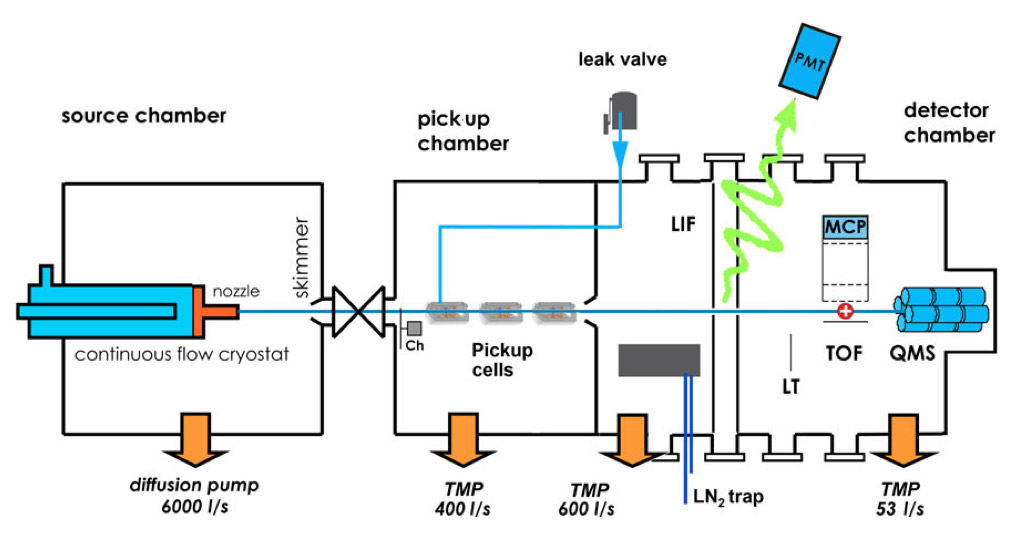
\includegraphics[width=13cm]{./experimental_setup/scheme.jpg}}
\captionabove{\label{apparatus-scheme} \textsl{The three main chambers are shown schematically, with measurement devices and pumps. Taken from  \cite{lackner-doc}. }}
\end{figure}

The following abbreviations were used in figure \ref{apparatus-scheme}:

\textit{TMP ... Turbo molecular pump} \\
\textit{Ch  ... Chopper} \\
\textit{PMT ... Photomultiplier tube} \\
\textit{LIF ... Laser induced florescence spectroscopy setup} \\
\textit{TOF ... Time-of-flight mass spectrometer} \\
\textit{QMS ... Quadrupole mass spectrometer}
%\textit{LT ... Laser}

The blue line, reaching from the nozzle to the end of the detection chamber, represents the helium droplet beam. The beam is created via a supersonic gas expansion through the $\unit[5]{\mu m}$ nozzle. A $\unit[400]{\mu m}$ skimmer at the end of the source chamber extracts the helium nanodroplets which pick up the dopants in the subsequent pick up chamber. The measurements are done in the detection chamber. The apparatus is equipped with many detection devices, important for this work are the LIF-spectroscopy setup and the TOF- and QMS mass spectrometer, which are described in detail in section \ref{chap:methods}.


\section{Source chamber}
\vspace{-1\baselineskip}
High purity helium gas (Air Liquide, Alphagaz 2 He B50L L, He>=99.9999\%) is used for the preparation of He$_N$ clusters in a supersonic gas expansion. In our experiments the gas is typically forced through the nozzle with a pressure of $\unit[60]{bar}$. An oil diffusion pump (Leybold D1 6000 10B) holds the vacuum pressure of the source chamber at $\unit[10^{-6}]{mbar}$ if no helium beam is present and at $\approx \unit[10^{-4}]{mbar}$ if the beam is established \cite{krois}. In order to form droplets, the gas is cooled to temperatures below $\unit[25]{K}$ within a heat exchanger (figure \ref{precooling}). The gas inlet for the high purity helium is wound around the outer steel pipe which is cooled by gaseous helium from an external dewar filled with liquid helium ($\unit[4]{K}$). The cooling has to be maintained during the whole experiment. To ensure constant nozzle temperatures the apparatus is equipped with a Lakeshore 330 Autotuning controller which heats the nozzle when needed. The typical nozzle temperature in our RbSr experiments is $\unit[15]{K}$.

\begin{figure}[ht]
\centerline{
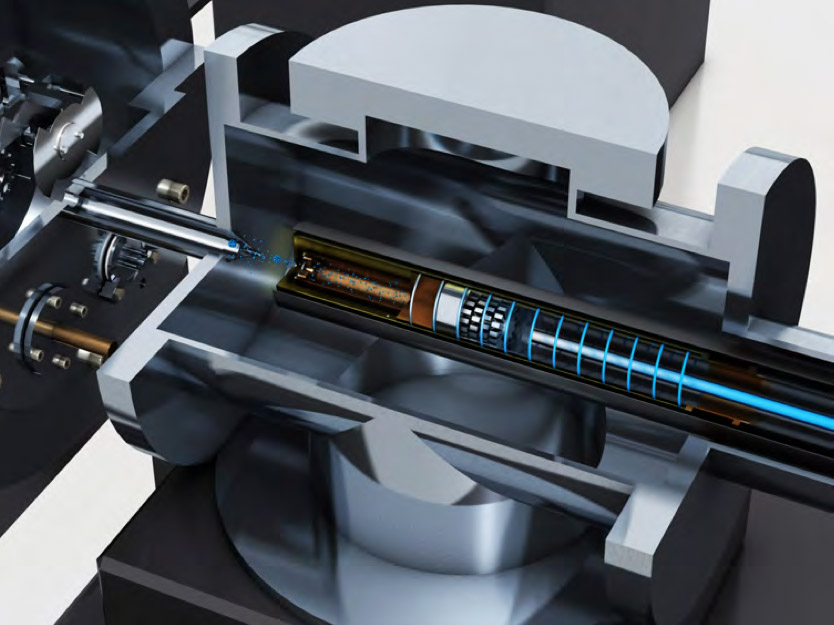
\includegraphics[width=12cm]{./experimental_setup/pre_cooling.jpg}}
\captionabove{\label{precooling} \textsl{Heat exchanger to cool the high purity helium (spiral wire) and the nozzle to temperatures of about $\unit[15]{K}$ \cite{krois}. }}
\end{figure}


\section{Pick up chamber}
\vspace{-1\baselineskip}
The pick up chamber contains different pick up cells in order to dope the helium droplets with gaseous or solid species. The chopper at the entry of this chamber is important for the alignment process of the nozzle. It is a rotating disk which interrupts the helium beam periodically to distinguish between background and actual helium beam (measured with the QMS). The background is the effusive beam of dopants which reaches the detection chamber even without a helium beam. %It allows to differ between background and signal in a QMS signal. The background is the effusive beam of dopants which reaches the detection chamber even without a helium beam (closed chopper).
%the helium nanodroplet beam is chopped by a rotating disk.
%Once a helium signal is present it is maximized through changing the position of the nozzle vertically as well as horizontally. The chopper only rotates during this alignment process. After that the chopper is stopped and the helium beam can pass uninterrupted. It is very important to double check the position of the stopped chopper, because the controller is not reliable in terms of the ''Stop Open'' position. \\
Figure \ref{pickup-chamber} shows the arrangement within the chamber with chopper and the three different pick up cell types.

\begin{figure}[ht]
\centerline{
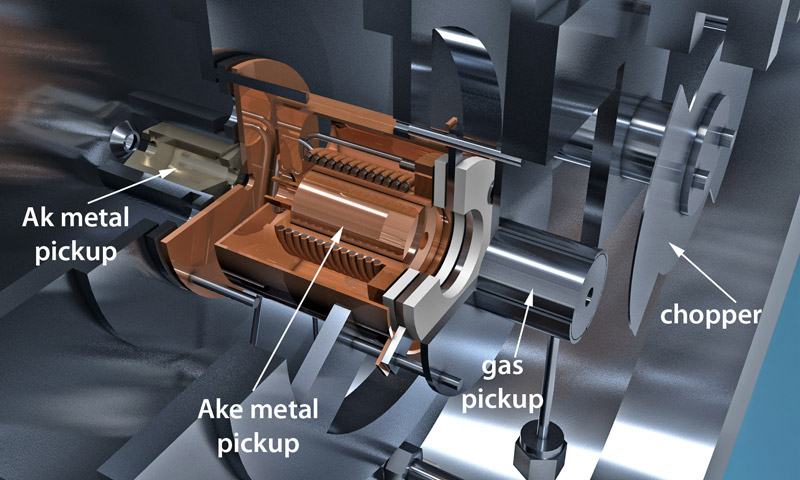
\includegraphics[width=13cm]{./experimental_setup/pickup-chamber.jpg}}
\captionabove{\label{pickup-chamber} \textsl{The pick up chamber with chopper and available pick up cell types. Beam enters from the right. Taken from \cite{krois}. }}
\end{figure}

The first cell is used for doping with gaseous dopants. It is designed as a steel cylinder with an external gas inlet. Because the dopants are already gaseous no heating is required in this case.
In contrast to this cell type the other two pick up cells in figure \ref{pickup-chamber} are able to evaporate solid species. The alkali metal oven is a steel cylinder with a reservoir for solid species. The cell is connected to an external power supply, controlled by an Eurotherm temperature controller. \\
The alkaline earth metal oven, designed by G\"unter Krois, provides several improvements of the steel cylinder type, discussed in detail in \cite{krois}. It is made out of copper to react faster to changes of the heating current and to be more efficient. The cell has a temperature shield, which is connected to a thick copper wire transporting heat outside of the apparatus. The shield minimizes the influence on cells nearby which is important because the available room in the pick up chamber is very limited.

A turbo molecular pump holds the vacuum pressure in the chamber at $\unit[10^{-7}]{mbar}$. Vapor pressures in the pick up cells of about $\unit[10^{-3}-10^{-4}]{mbar}$ are sufficient for the pick up process. In the case of rubidium and strontium, cell temperatures of $\unit[\approx 80]{^\circ C}$ and $\unit[\approx 420]{^\circ C}$ are needed to reach those pressures.

After the doping process, the droplets enter the detection chamber where the experiments are performed.


\section{Detection chamber}
\vspace{-1\baselineskip}
The detection chamber is equipped with the measuring devices and is the last of the three subsequent chambers. A set of pumps holds the vacuum pressure of the chamber in the low range of $\unit[10^{-7}]{mbar}$. Figure \ref{detection-chamber} shows the arrangement of the LIF spectrometer and the TOF and QMS mass spectrometers.

\begin{figure}[ht]
\centerline{

\includegraphics[width=15cm]{./experimental_setup/detection-chamber.jpg}}
\captionabove{\label{detection-chamber} \textsl{Detection chamber with TOF and QMS mass spectrometer and LIF spectrometer. Modified from \cite{krois}. }}
\end{figure}

% The following gives a short overview of the devices before the next section will describe the two mainly used measuring methods in more detail.
For LIF spectroscopy the photomultiplier tube (PMT) is used to detect florescence light. It is possible to replace the PMT with a grating spectrograph for dispersed florescence measurements. \\
The TOF mass spectrometer extracts ions after laser ionization and measures their different flight times (due to different masses). \\
The QMS is located at the end of the apparatus and was mainly used to align the nozzle and the helium beam. A QMS uses an inhomogeneous electrical field, established by four parallel rods, to select ions according to their m/q ratio.
%LIF measurements (Laser Induced Fluorescence) are done with a Photo Multiplier Tube (PMT) which detects fluorescent light and can be exchanged with a grating spectrograph when needed. \\
%The time-of-flight spectrometer (TOF) extracts ions after laser ionization with an electrical field and detects them due to their different flight times. \\
%The quadrupole mass spectrometer (QMS) is at the end of the apparatus (in beam direction) and is mainly used to align the helium droplet beam. A QMS uses an inhomogeneous electrical field, established by four parallel plates, which selects ions according to their m/q ratio.

The measuring methods, relevant for this work, are explained in the following.
\newpage
\section{Measuring methods}
\label{chap:methods}
\vspace{-1\baselineskip}
In this section an overview of LIF spectroscopy and REMPI-TOF mass spectroscopy is given. Detailed informations about these methods are found in the referenced literature \cite{demtr-laser} \cite{lackner} \cite{lackner-doc}.


\subsection{REMPI-TOF spectroscopy}
\vspace{-1\baselineskip}
%\underline{REMPI-TOF} \\
REMPI-TOF spectroscopy (Resonance Enhanced Multi Photon Ionization) was used in order to record excitation spectra in the RbSr and Au experiments. Neutral dopants on the helium droplet are ionized by incident laser photons. Ionization is either possible via one-, two- or multi photon processes. In a one photon process, a single photon ionizes an atom or molecule directly from the ground state. In a two photon process the first photon excites into a virtual or resonant intermediate state while the second photon ionizes. If the excited intermediate state is a real atomic or molecular state the process is called resonant (resonant two photon ionization - R2PI). The ionization probability is much higher via resonant states with long life-times. Ideally the life-time is longer than the pulse duration of the laser. %The transition rate for multi photon processes can be increased with higher laser powers. While the transition rate for one photon processes is linear to the laser power it is quadratic for two photon processes: $P \propto I^2$.

%\underline{REMPI-TOF} \\
For the experiments presented in this thesis, the two photon process via resonant energy levels is the most relevant one. In this case the wavelength of a tunable laser (Lambda Physik FL 3002 or Coherent Indigo-S) is tuned across resonant energy states. A second laser photon ionizes the atom from the resonant state. Ionization is done either with a fraction of the intensity of the pump laser (Radiant Dyes RD-EXC 200 XeCl laser, $\unit[308]{nm}$) or with a second photon of the dye laser. During the ionization process, the dopants desorb from the droplets and are subsequently extracted by the electric field of the TOF. The TOF accelerates the ions towards a detector where they arrive at different time intervals. Ions per time-intervall are counted. The time of flight is measured from the beginning of each laser pulse. Typically the laser is operated with a repetition frequency of $\unit[100]{Hz}$ ($\unit[5]{kHz}$ in case of the Indigo-S) and triggers the counter of the TOF. In case the dye laser excites into a resonant state the ion yield increases, resulting in an excitation spectrum of the dopant in a specific spectral range. \\
Note that for better resolutions the TOF is operated in reflectron mode. Figure \ref{tof-ref} shows the TOF set up in reflectron and linear mode. \\

\begin{figure}[ht]
\centerline{
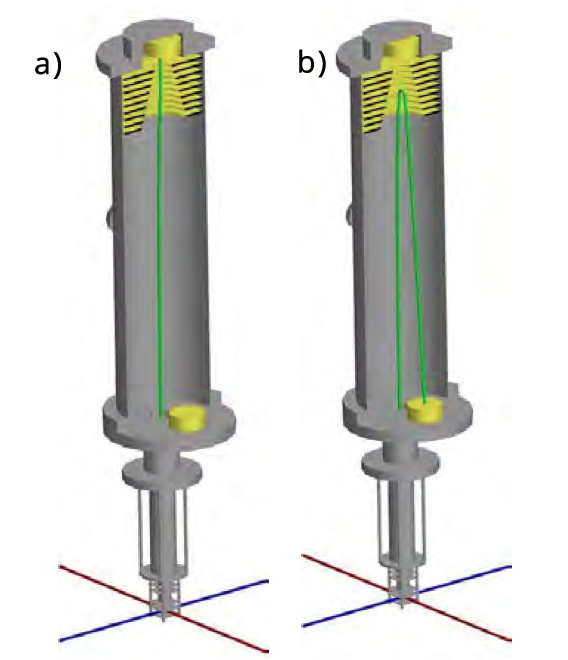
\includegraphics[width=7cm]{./measuring_methods/tof-lin-ref.jpg}}
\captionabove{\label{tof-ref} \textsl{a) TOF in linear mode and b) in reflectron mode. Taken from \cite{krois}. }}
\end{figure}
%In our experiments the dye laser is not set to a fixed wavelength. Instead the laser is scanned over a certain wavelength range where transitions are assumed. The transition rate and therefore the ionization rate is much higher for wavelengths meeting the energy difference of real states. This increase in the ion yield is detected with the TOF spectrometer. In that way the REMPI-TOF method let us find new transitions and gives us a good starting point for further investigations via LIF spectroscopy.

\subsection{Laser induced florescence spectroscopy}
\vspace{-1\baselineskip}
Laser induced fluorescence is the spontaneous emission of light caused by relaxation of electrons after laser excitation. The emitted fluorescent light is collected by a lens system (shown in figure \ref{lif-setup}) and recorded with a photo multiplier tube (PMT, Hamamatsu R943-01) which is not wavelength dispersive. LIF gives excitation spectra similar to REMPI-TOF spectra, is not mass selective, but more sensitive. \\
When recording excitation spectra a laser is scanned over resonant states. Figure \ref{lif-vib} shows different possible relaxations after laser excitation. All emitted photons are detected with a PMT and according to the Franck-Condon factors certain transitions are more likely than others, giving differences in the measured intensities.

\begin{figure}[ht]
\centerline{
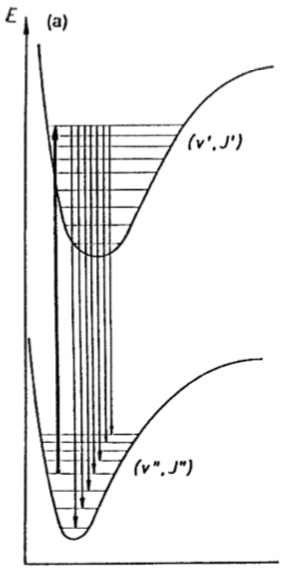
\includegraphics[width=5cm]{./measuring_methods/lif-vib.jpg}}
\captionabove{\label{lif-vib} \textsl{Relaxation from an excited state into vibrational levels of the ground state. Taken from \cite{demtr-laser}. }}
\end{figure}

To investigate the relaxation process in more detail, dispersed fluorescence spectroscopy is used. For this experiment, the PMT is exchanged by a grating spectrograph. A cw dye laser is used for high intensities at a specific wavelength. The cw laser excites exclusively into resonant states.
\begin{figure}[ht]
\centerline{
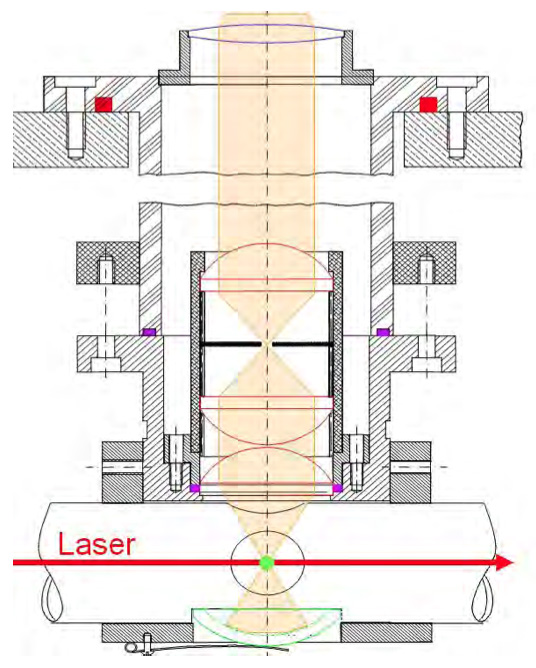
\includegraphics[width=9cm]{./measuring_methods/lif-setup.jpg}}
\captionabove{\label{lif-setup} \textsl{Setup for LIF-spectroscopy within the apparatus. Taken from \cite{lackner}. }}
\end{figure}
Every relaxation depicted in figure \ref{lif-vib} causes emission of a photon with a specific wavelength. These photons are collected by a lens system depicted in figure \ref{lif-setup} and guided into the grating spectrograph. A cooled CCD chip (LOT-Andor iDUS DU401ABR-DD) detects the photons and sends the signal to the computer. \\
Note that a reflector underneath the interaction zone increases the number of photons reaching the detector. To minimize the influence of scattered light the laser is guided through a baffle tube.

%Whereas the excitation measurements (REMPI-TOF) gave informations about excited states, emission measurements (LIF) investigate the ground state of an atom or molecule.

\chapter{Experimental Results}
\label{chap:results}
\vspace{-1\baselineskip}
This chapter informs about the results of our experiments, carried out in the course of this thesis. The first part of the chapter is dedicated to the RbSr experiments in Cluster Lab I. The second part reports on the results of the gold experiments done in Cluster Lab III. While different experimental setups were used in the laboratories, this chapter presents REMPI-TOF spectra for RbSr as well as for Gold on and in He$_N$. Differences in the experimental setup are described in section \ref{chap:auex} and chapter \ref{chap:goldoven}.

\section{RbSr Experiments}
\label{chap:rbsrresults}
\vspace{-1\baselineskip}
In the course of this work, which is also part of the PhD thesis of G\"unter Krois (ref. \cite{krois-doc}), we investigated the RbSr molecule on the surface of helium nanodroplets. The spectroscopic results were obtained with REMPI-TOF as well as LIF spectroscopy and have been published in refs. \cite{paperlackner} and \cite{paperkrois}. This section is based on the referenced papers. The theoretical data, used to compare the experiments with calculations, are based on the PhD thesis of Johann V. Pototschnig, ref. \cite{johann-doc} \\
All experiments regarding the RbSr molecule were performed in Cluster Lab I at the Institute for Experimental Physics in Graz. The experimental setup of this apparatus is described in chapter \ref{chap:expsetup}.

RbSr is an alkali-alkaline earth molecule which is hard to form and to investigate. The helium nanodroplet method enables the formation of the molecule on the surface of the cluster. The two atoms are picked up sequentially by the droplet and their long-reaching van der Waals forces lead to attraction, followed by formation of the molecule. The binding energy freed by this process ($\approx \unit[1000]{cm^{-1}}$, ref. \cite{zuchowski}) causes evaporation of about 200 helium atoms - assuming $\unit[5]{cm^{-1}}$ binding energy between a helium atom and the droplet (ref. \cite{toennis}). Both atoms have several isotopes which makes the mass spectra more complex. The natural isotope distribution of Rb is $72.18\%$-$^{85}$Rb and $27.82\%$-$^{87}$Rb. Sr has three isotopes with an isotopic abundance of $9.86\%$-$^{86}$Sr, $7.0\%$-$^{87}$Sr and $82.58\%$-$^{88}$Sr, see ref \cite{crc}. Therefore mass peaks for dimers and diatomic molecules in the REMPI spectrum can contain contributions from more than only two specific isotopes. This is shown in figure \ref{rbsrmasses}. The green bars illustrate the percentage of Rb atoms whereas the magenta ones show the contribution of Sr atoms. The blue bars in the right diagram represent the RbSr molecule. The mass spectrum shown in figure \ref{rbsrmasses} was taken during the REMPI-TOF recording of the $4 ^2\Sigma^+ \leftarrow X ^2\Sigma^+$ transition.
\begin{figure}[ht]
\centerline{
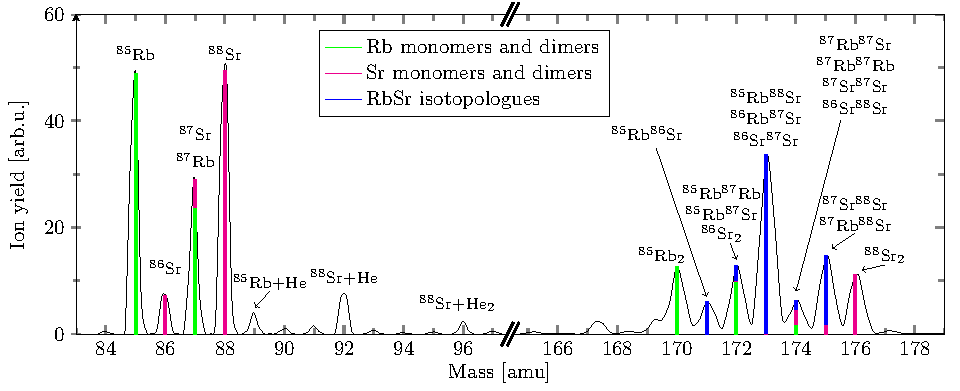
\includegraphics[width=16cm]{./resultsRbSr/rbsr_masses.pdf}}
\captionabove{\label{rbsrmasses} \textsl{Example of a REMPI-TOF mass spectrum showing Rb and Sr monomers on the left and dimers and the RbSr molecule on the right. The black graph is the ion yield recorded with the TOF-spectrometer. The green and magenta bars show the contribution of the atoms Rb and Sr respectively, whereas the blue bars represent the RbSr molecule. Taken from ref. \cite{paperkrois} }}
\end{figure}

During the experiments we found an optimum pickup temperature of about $\unit[80]{^\circ C}$ for Rb and $\unit[420]{^\circ C}$ for Sr. If not stated otherwise all spectra were recorded at these temperatures. For REMPI-TOF spectra a dye laser (Lambda Physik FL 3002) was used to excite the dopants and a fraction of the pump laser (Radiant Dyes RD-EXC 200 XeCl laser, $\unit[308]{nm}$) was used to ionize them. Our results cover a spectral range from $\unit[11600]{cm^{-1}}$ - $\unit[23000]{cm^{-1}}$ (overview in figure \ref{rbsroverview}). From an energy of $\unit[14700]{cm^{-1}}$ upwards, two photons of the dye laser are sufficient to ionize RbSr. All REMPI-TOF spectra were recorded with the Jordan D-850 AREF TOF with angular reflectron and show ion yield versus dye laser wavelength. The RbSr transition around $\unit[14200]{cm^{-1}}$ was also investigated with LIF spectroscopy using a photomultiplier tube (Hamamatsu R943-01). %This transition ($4 ^2\Sigma^+ \leftarrow X ^2\Sigma^+$) is described at the end of the RbSr section in more detail.

\begin{figure}[ht]
\centerline{
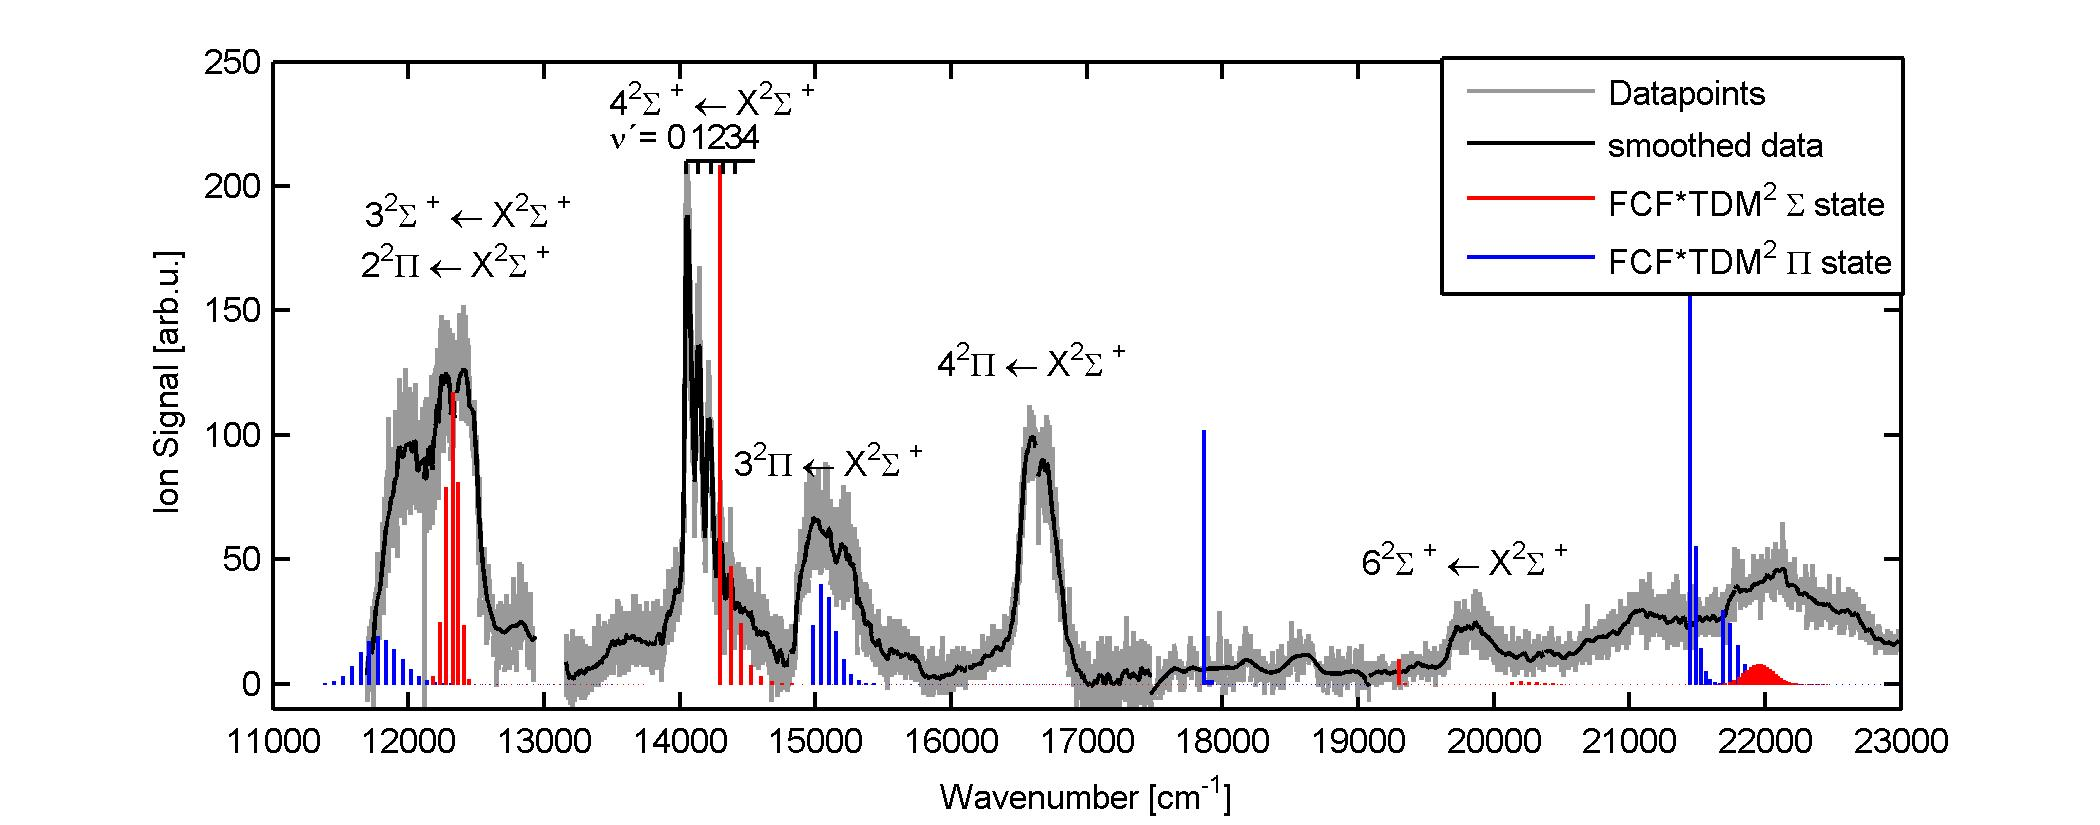
\includegraphics[width=18cm]{./resultsRbSr/overview.jpg}}
\captionabove{\label{rbsroverview} \textsl{Overview of the transitions within the available spectral range. The gray graph represents the data points whereas the black line corresponds to the smoothed data. Red and blue are the transition probabilities for the $\Sigma$ and $\Pi$ states respectively. \cite{paperlackner} }}
\end{figure}

The overview in figure \ref{rbsroverview} shows several transitions within the available spectral range. The gray graph represents the data points whereas the black line corresponds to the smoothed data. Red and blue are the products of the Franck-Condon factors (FCF) times the squared transition dipole moment (TDM) for the $\Sigma$ and $\Pi$ states. In the following this product is referred to as ''transition probability''. The calculated transition probabilities make it possible to assign peaks to transitions. \\
The $4 ^2\Sigma^+ \leftarrow X ^2\Sigma^+$ transition is the only vibrationally resolved one and is described in more detail in the end of this section. The other transitions, denoted in figure \ref{rbsroverview}, appear as broad structures which do not allow the identification of individual features. The double peak at $\unit[12000]{cm^{-1}}$ is in agreement with the theoretical transition probabilities (shown as red and blue bars) suggesting two overlapping transitions. The peak at lower energy is identified as the $2 ^2\Pi \leftarrow X ^2\Sigma^+$ transition. The peak at higher energy corresponds to the $3 ^2\Sigma^+ \leftarrow X ^2\Sigma^+$ transition. Both transitions correlate to the atomic asymptote of the energies of the Rb 5s $^2$S ground state and the Sr 5s5p $^3$P excited state (figure \ref{rbsrpot}). \\
The structure at $\unit[15000]{cm^{-1}}$ is assigned to the $3 ^2\Pi \leftarrow X ^2\Sigma^+$ transition. \\
For excited states above $\unit[16000]{cm^{-1}}$, figure \ref{rbsroverview} shows that the results of experiment and theoretical calculations differ. We know that the theoretical calculations overestimate the $4 ^2\Pi \leftarrow X ^2\Sigma^+$ transition and underestimate the $6 ^2\Sigma \leftarrow X ^2\Sigma^+$. The proximity of Rb and Sr levels in this energy range and an increasing density of molecular states make theoretical calculations increasingly difficult. The known deviations for the two transitions are in good accordance to the experimental results. The $4 ^2\Pi \leftarrow X ^2\Sigma^+$ transition is overestimated by about $\unit[1000]{cm^{-1}}$ whereas the $6 ^2\Sigma \leftarrow X ^2\Sigma^+$ is underestimated by about $\unit[200]{cm^{-1}}$.

Figure \ref{rbsrpot} shows the potential energy curves for the $\Pi$ and $\Sigma$ states of the RbSr molecule in the investigated energy range, ref. \cite{krois-doc}. The minimum of the RbSr ground state is at $\unit[-1000]{cm^{-1}}$. The excited $\Sigma$ states are denoted in the graphic (red curves). The lowest $\Pi$ states are the $1 \ ^2\Pi$ state with the potential minimum at about $\unit[3750]{cm^{-1}}$ and the $2 \ ^2\Pi$ state with the minimum at $\unit[10000]{cm^{-1}}$. The corresponding atomic asymptotes are denoted on the right side of the graphic.

\begin{figure}[ht]
\centerline{
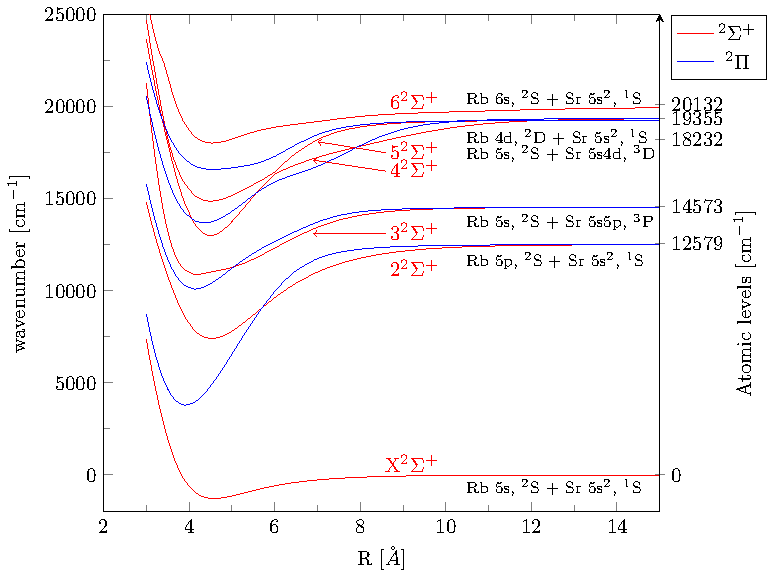
\includegraphics[width=16cm]{./resultsRbSr/MolSpec_PECs.pdf}}
\captionabove{\label{rbsrpot} \textsl{Potential energy curves of the RbSr molecule in the investigated energy range. Red curves represent the $\Sigma$ states and blue curves the $\Pi$ states. Taken from \cite{johann-doc} }}
\end{figure}

\newpage

\underline{$4 \ ^2\Sigma^+ \leftarrow X \ ^2\Sigma^+$ transition} \\
The $4 \ ^2\Sigma^+ \leftarrow X \ ^2\Sigma^+$ transition at $\unit[14200]{cm^{-1}}$ was investigated with TOF and LIF spectroscopy. The resulting spectra are shown in figure \ref{toflif}. The figure is divided into three sections. In a) the gray line shows the REMPI-TOF ion yield. The red graph represents the smoothed data. Green denotes the fitted signal. %A sum of asymmetric 2$\Sigma$ functions was used as a fitting function.
The signal shows five peaks corresponding to the vibrational transitions $\nu'=0-4 \leftarrow \nu''=0$. Due to the low temperature of about $\unit[0.37]{K}$, every excitation starts at the vibrational ground state of the molecule ($\nu''=0$). The peaks show an asymmetric broadening to higher energies, caused by strong interactions with the droplet. This results in a lambda shaped peak form.

\begin{figure}[ht]
\centerline{
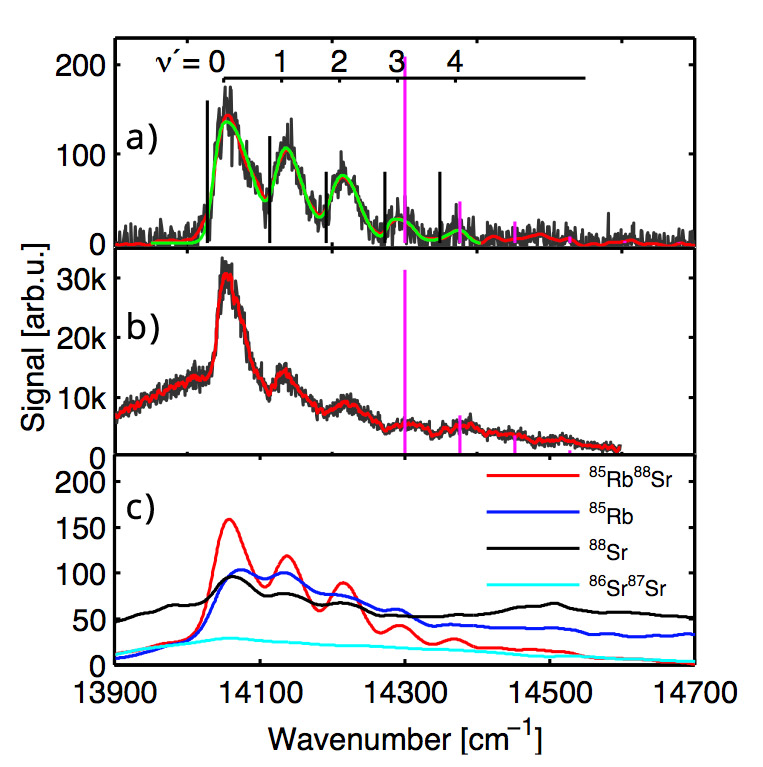
\includegraphics[width=13cm]{./resultsRbSr/liftof.jpg}}
\captionabove{\label{toflif} \textsl{The $4 ^2\Sigma^+ \leftarrow X ^2\Sigma^+$ transition in detail. a) REMPI-TOF spectrum. Gray shows the original ion yield, red the smoothed and green the fitted data. The black vertical lines mark the onset of the rising edges of the corresponding free molecule transitions. b) shows the LIF spectrum for the transition. c) A comparison of different REMPI-TOF signals to investigate the cause of the background shown in b). The cyan Sr$_2$ signal was recorded in a separate experiment.}}
\end{figure}

Section b) in figure \ref{toflif} shows the LIF spectrum of the vibrational transitions $\nu'=0-4 \leftarrow \nu''=0$. In this case the $\nu'=0 \leftarrow \nu''=0$ is much higher than the other four transitions. The signal height fits the calculated transition probabilities, denoted as vertical bars, better in the LIF experiment. But it also shows an underlying background, shifting the spectrum upwards. The cause of this background is a Sr dimer transition which is shown in figure \ref{toflif} c). The figure shows the molecule $^{85}$Rb$^{88}$Sr (red), and the single atoms $^{85}$Rb (blue) as well as $^{88}$Sr (black). The cyan line represents the REMPI-TOF signal of the $^{88}$Sr$^{87}$Sr molecule recorded in an experiment optimized for Sr$_2$ pickup. This signal clearly shows an increase in the range of the background (b), indicating a Sr$_2$ transition. To minimize the influence of Sr dimers and trimers, the pick up temperature was lowered.

\newpage

\section{Au experiments}
\vspace{-1\baselineskip}
\label{chap:auex}
Gold is an outstanding material among the metal atoms and has many technical applications in electronics, optics and material science. With the rise of nanotechnology gold attracted even more interest, especially in life sciences (see refs. \cite{biogold1}, \cite{biogold2}). Fundamental research on gold can therefore yield to benefits in several scientific fields, not only physics. Despite these promising prospects, spectroscopic data for gold atoms in helium nanodroplets are not available. Moroshkin et al. presented emission spectra in solid and liquid helium matrices, but did not include an investigation of the $5d^{10} 6p \ ^2P^o_{1/2} \leftarrow 5d^{10} 6s \ ^2S_{1/2}$ transition \cite{moroshkin}. In contrast, the elements silver and copper, with similar electron configurations, have already been investigated in He$_N$ clusters (refs. \cite{loginov2007excited} and \cite{cufritz}).
It was part of this thesis to obtain the first spectra of gold atoms in helium nanodroplets. The following section reports on the results.
% Basically the gold atom itself is comparable with elements like silver or copper, both already investigated \cite{loginov2007excited} \cite{cufritz}.
%The ground state of gold is written as $[Xe]5d^{10}6s$. Figure \ref{autrans} shows the Gotrian diagram for the ground state and relevant excited states. The ionization limit is at $\unit[74 409.11]{cm^{-1}}$.

The gold experiments were performed in Cluster Lab III at the Institute of Experimental Physics in Graz. The apparatus in this laboratory is designed to investigate very large clusters of up to $\unit[10^6]{amu}$. For this reason the apparatus is able to vary the stagnation conditions over a wide range. Nozzle temperatures of about $\unit[3.8]{K}$ (at $\unit[20]{bar}$) and helium pressures up to $\unit[100]{bar}$ are possible. The principle setup of the apparatus is very similar to the one used in the RbSr experiments (chapter \ref{chap:expsetup}). Therefore only the main differences to the apparatus in Cluster Lab I are listed below:

\begin{itemize}
\item The nozzle is cooled with a cold head which can be controlled via a PC.
\item A high temperature oven, described in chapter \ref{chap:goldoven}, was used as pick up source.
\item The apparatus is equipped with a TOF mass spectrometer with angular reflectron (Kaesdorf RFT50), a QMS and a micro balance. For the experiments in this section, only the TOF mass spectrometer was used.
\end{itemize}

Although REMPI spectra were the main focus of our experiments, we also obtained mass spectra with electron impact ionization. In the latter case atoms and clusters are ionized by high-energy electrons instead of laser photons. The electron energies ($\unit[89]{eV}$) are high enough to ionize helium atoms in the cluster. A charge hopping mechanism within the droplet leads to ionization of Au$_n$. The ionized complexes are then extracted by the electrical field of the TOF, similar to the REMPI-TOF experiments. Figure \ref{masslaseregun} shows a comparison of two mass spectra obtained with electron impact ionization (top) and laser ionization (bottom) recorded at the same stagnation and pick up conditions. In the spectrum obtained with electron impact ionization the masses for Au ($\unit[197]{amu}$), Au$_2$ ($\unit[394]{amu}$), Au$_3$ ($\unit[591]{amu}$), Au$_4$ ($\unit[788]{amu}$) and Au$_5$ ($\unit[985]{amu}$) are identifiable in the depicted range. The equidistant (\unit[4]{amu}) peaks which, follow Au$_n$ peaks, originate from helium atoms attached to the respective element (for example AuHe, AuHe$_2$, AuHe$_3$,...). This is called ''helium comb''. Because the energy of the electrons is high enough to ionize pure helium, a helium comb is also observed for masses lower than $\unit[197]{amu}$.

\begin{figure}[ht]
\centerline{
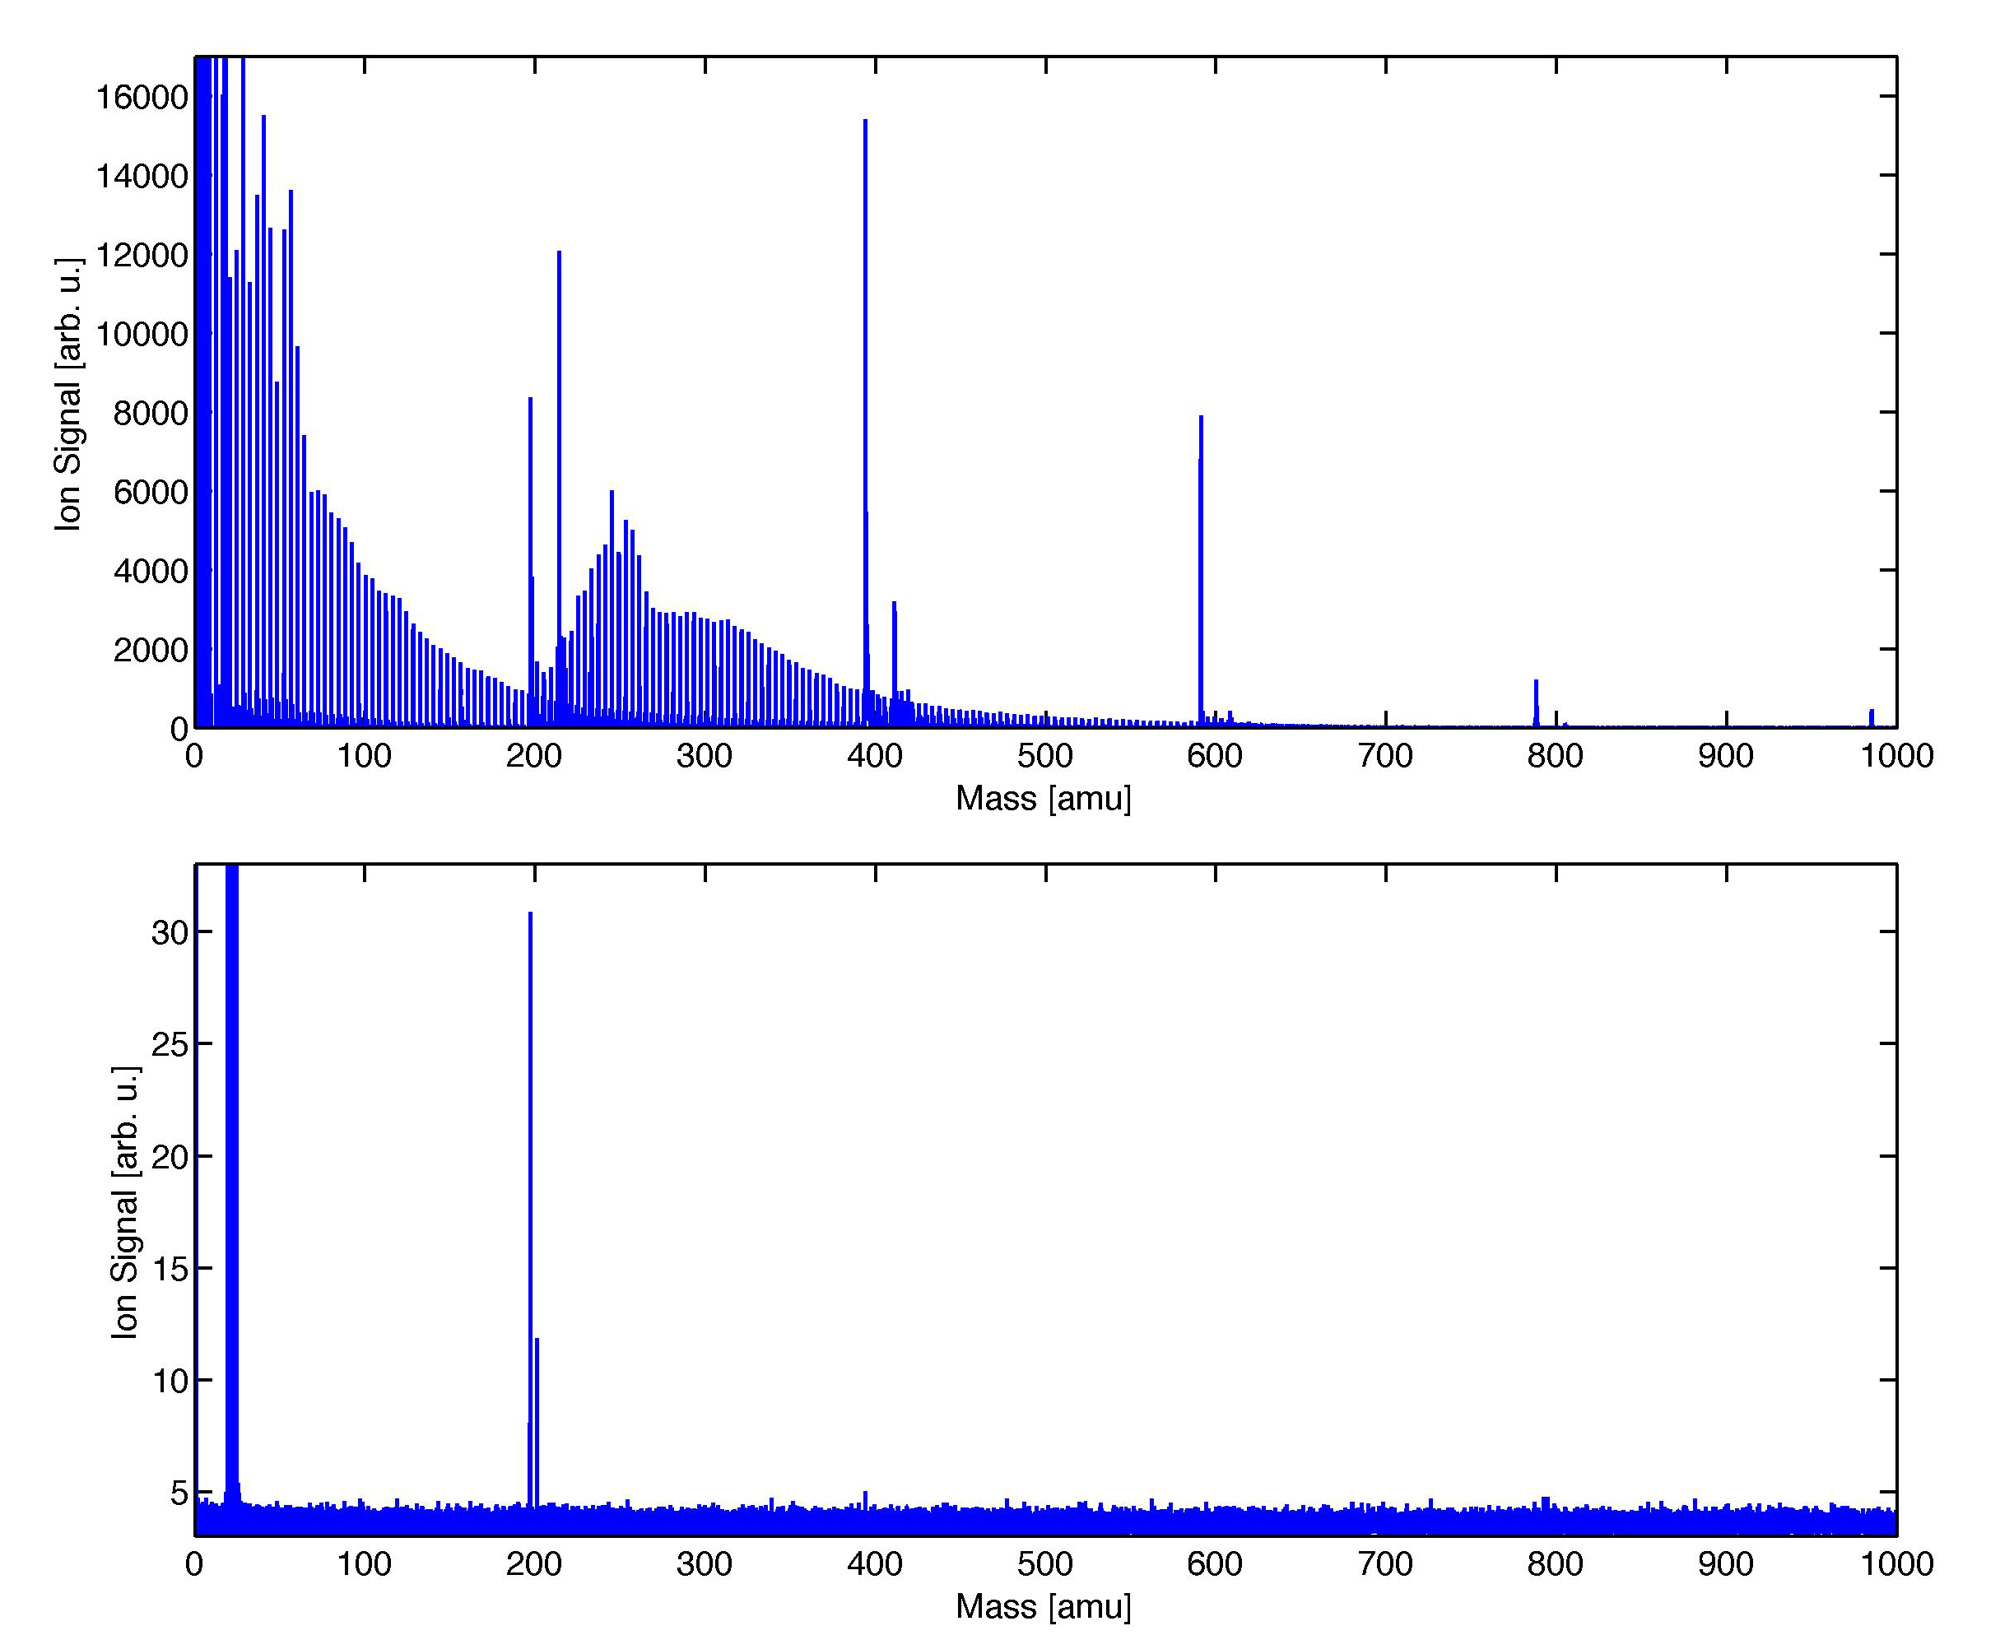
\includegraphics[width=16cm]{./results/mass_egun_laser.jpg}}
\captionabove{\label{masslaseregun} \textsl{Comparison of two mass spectra obtained with electron impact ionization (top) and laser ionization (bottom). Electron impact ionization gives higher ion yields, shows larger clusters and helium comps. }}
\end{figure}

The mass spectrum obtained with laser ionization (figure \ref{masslaseregun}, bottom) was summed over all recorded wavelengths ($\unit[37200]{cm^{-1}}$ to $\unit[40000]{cm^{-1}}$) and divided by the number of spectra. It shows peaks for Au ($\unit[197]{amu}$), AuHe ($\unit[201]{amu}$) and Au$_2$ ($\unit[394]{amu}$). Larger Au$_n$ clusters were not observed.

In the following only spectra obtained with laser ionization are discussed. Because the gold experiments were the first spectroscopic investigations in this laboratory, a laser system had to be installed. To cover the wavelength range from $\unit[37200]{cm^{-1}}$ to $\unit[40000]{cm^{-1}}$ the Indigo-S laser, from Cluster Lab I, was set up. The following provides a short introduction into this laser. More details can be found in refs. \cite{lackner} and \cite{pifrader}.

\underline{The Indigo-S laser} \\
The Indigo-S is a Ti:sapphire laser pumped by a pulsed Coherent Evolution-15 laser. The pump laser produces pulses with a repetition rate of $\unit[5]{kHz}$ ($\unit[200]{\mu s}$ pulse distance, $\unit[29]{ns}$ pulse duration). The Evolution-15 laser consists of a diode pumped Nd:YLF crystal, operated in Q-switch mode. In this mode the diode populates the upper laser level of the active medium until the population inversion reaches a maximum. Oscillation is prevented through high losses in the resonator. In that way the Evolution-15 provides short laser pulses with high output powers at $\unit[1064]{nm}$ which are frequency doubled to $\unit[532]{nm}$. The pulses of the Evolution laser pump a Ti:sapphire laser with a fundamental wavelength of $\unit[750-920]{nm}$. During the gold experiments the "$\unit[193]{nm}$"-mirror set (name by Coherent) was used to cover a fundamental wavelength range of $\unit[750-840]{nm}$. With subsequent crystals the frequency of the fundamental beam can be doubled ($\unit[375-420]{nm}$) and tripled to reach the desired range of $\unit[250-280]{nm}$. Because laser power varies over wavelength it was measured externally with a power-meter. The wavelength was measured with the internal spectrometer of the Indigo-S laser. An external wavemeter could not be used over the entire wavelength range, because the broad mode structure of the laser forbids an exact determination of the wavelength.

\newpage

\subsection{REMPI spectra}
\label{chap:aurempi}
\vspace{-1\baselineskip}
REMPI spectra are obtained by ionizing Au-He$_N$ clusters with the Indigo-S laser and measuring the ion yield with a time-of-flight mass spectrometer (Kaesdorf RFT50). The electron configuration of gold in its ground state is [Xe] 4f$^{14}$5d$^{10}$6s$^1$. In this state gold has closed f- and d-shells and one 6s valence electron. This configuration makes gold comparable to the alkali metals. \\
The strongest gold transition from the ground state into the excited $5d^{10} 6p \ ^2P^o_{1/2}$ state corresponds to an energy of $\nu_1 = \unit[37 359]{cm^{-1}}$. This implies that a second photon, with the same energy, is already sufficient to ionize the atom ($2 \cdot \unit[37 359]{cm^{-1}} = \unit[74 718]{cm^{-1}}$, ionization threshold at $\unit[74 409.11]{cm^{-1}}$). This two-photon ionization scheme is illustrated in the Gotrian diagram in figure \ref{autrans}. The first arrow indicates a resonant one-photon excitation ($5d^{10}6p \ ^2P^o_{1/2} \leftarrow 5d^{10}6s \ ^2S_{1/2}$ ) with a wavelength $\nu_1$ and the second arrow indicates the ionization. The term values in figure \ref{autrans} were taken from the NIST database (ref. \cite{nist}) which also lists the life-time of the $5d^{10} 6p \ ^2P^o_{1/2}$ state with $\unit[6.1]{ns}$.

\begin{figure}[ht]
\centerline{
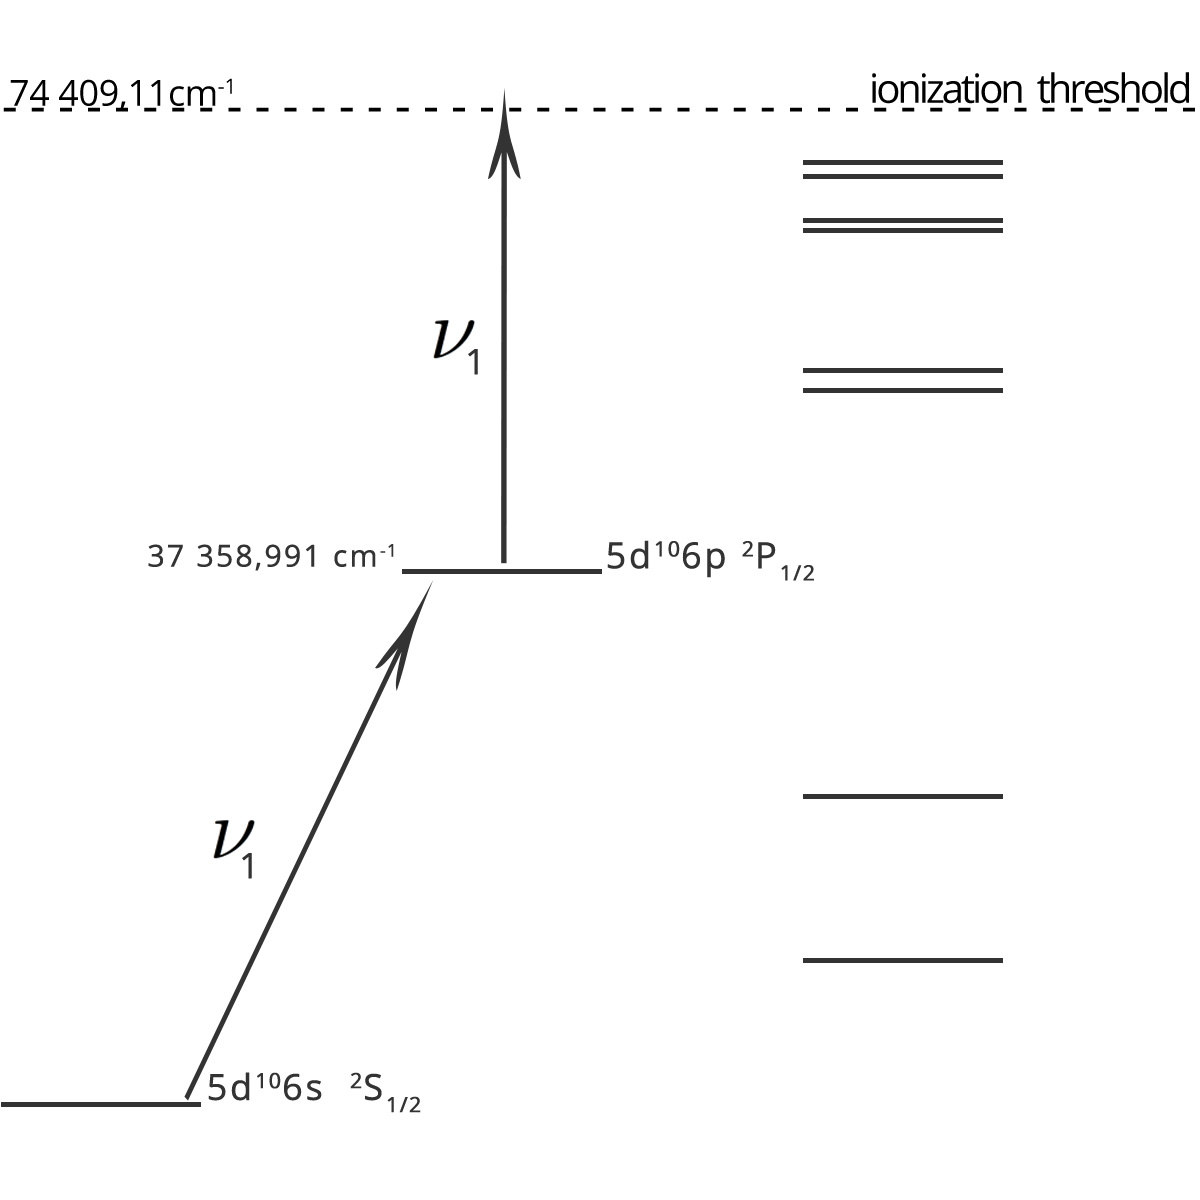
\includegraphics[width=8cm]{./results/au_trans_simple.jpg}}
\captionabove{\label{autrans} \textsl{Gotrian diagram showing the Au ground state (5d$^{10}$6s $^2$S$_{1/2}$) and the strongest transition into the $5d^{10}6p \ ^2P^o_{1/2}$ state with a life-time of $\unit[6.1]{ns}$. All energies correlate to the free atom.}}
\end{figure}

When obtaining REMPI spectra, the Indigo-S laser has the disadvantage that it can not be continuously tuned. Consequently, the spectra were taken at discrete wavenumbers in $\unit[2]{nm}$ and $\unit[0.6]{nm}$ steps. The latter corresponds to the minimal wavelength distance between two laser modes, accessible with the HR mirror of the Ti:sapphire resonator. The change from one laser mode to the next is done manually and causes a slight change in the laser path resulting in a displacement ($\approx \unit[0.5]{mm}$ at the TOF) which has to be corrected. Although iris diaphragms were used to mark the laser path, the realignment is not perfect, which affects the reliability of the recorded spectra.
Therefore the recorded spectra differ slightly, which makes the present interpretation speculative. In order to obtain more reliable spectra, the experiment has to be repeated to guarantee the reproducibility of the observed spectral features. \\
%Every measurement at a specific wavelength results in a REMPI spectrum for the entire mass range. To get spectra for a specific mass like Au, AuHe or AuHe$_2$ the ion signal at a specific wavelength is the sum .
Figure \ref{auspec} shows low-resolution REMPI spectra in $\unit[2]{nm}$ steps for Au (green), AuHe (blue) and 5 x AuHe$_2$ (red). \\
The most prominent feature of the Au signal is a very broad structure (FWHM $\approx \unit[790]{cm^{-1}}$) between $\unit[37350]{cm^{-1}}$ and $\unit[38400]{cm^{-1}}$. The width suggests that the transition occurs inside the droplet. The onset of the rising edge matches the position of the $5d^{10}6p \ ^2P^o_{1/2} \leftarrow 5d^{10}6s \ ^2S_{1/2}$ free atom transition exactly.
\begin{figure}[ht]
\centerline{
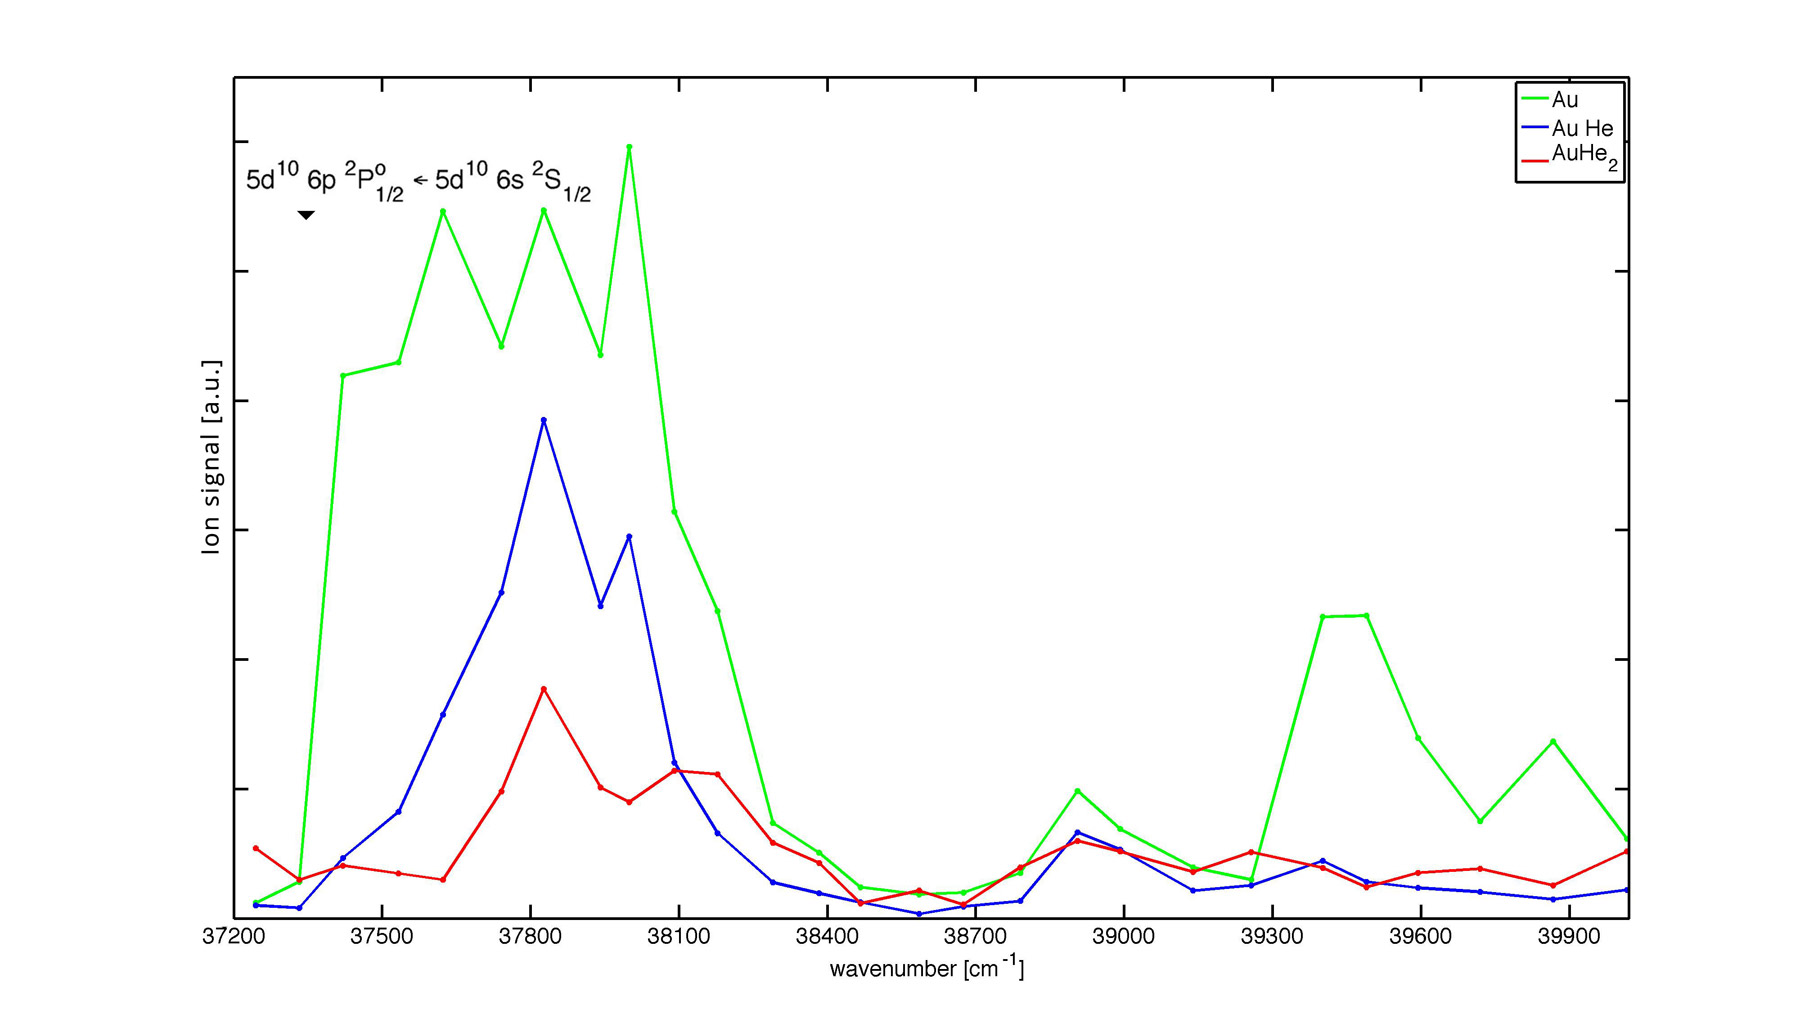
\includegraphics[width=17.5cm]{./results/au_spec_new.jpg}}
\captionabove{\label{auspec} \textsl{Low-resolution REMPI spectra for Au (green), AuHe (blue) and 5 x AuHe$_2$ (red). The Indigo-S laser was tuned in steps of $\unit[2]{nm}$. The energy of the atomic transition from the ground state into the $5d^{10}6p \ ^2P^o_{1/2}$ excited state is marked with a triangle. }}
\end{figure}

\newpage

To obtain more details about this structure a second spectrum, with smaller wavelength tuning steps of about $\unit[0.6]{nm}$, was recorded. This is the minimal step size of the Indigo-S laser without changing the position of the Etalon. Figure \ref{auspecfine} shows the Au spectrum obtained with $\unit[2]{nm}$ steps (green) in comparison to Au (magenta), AuHe (blue) and 3 x AuHe$_2$ (red) obtained in $\unit[0.6]{nm}$ steps and denoted with ''fine''. Whereas the low-resolution spectrum only showed a broad, featureless structure, the Au signal (magenta) now shows identifiable features. The signal shows a broad transition reaching from $\unit[37300]{cm^{-1}}$ up to about $\unit[38400]{cm^{-1}}$. This broad structure corresponds to the $5d^{10}6p \ ^2P^o_{1/2} \leftarrow 5d^{10}6s \ ^2S_{1/2}$ transition in the helium droplet. The onset of the rising edge is characteristically blue shifted to the atomic transition denoted in the figure with a black triangle.
\begin{figure}[ht]
\centerline{
\includegraphics[width=17cm]{./results/au_specFine_new.jpg}}
\captionabove{\label{auspecfine} \textsl{The spectrum compares the results obtained in $\unit[2]{nm}$ and $\unit[0.6]{nm}$ steps for Au (green and magenta). The spectra in $\unit[0.6]{nm}$ steps are denoted as ''fine''. AuHe and 3 x AuHe$_2$ are depicted in blue and red, respectively. The energies of the atomic transitions are marked with black triangles. }}
\end{figure}\\
On top of the $5d^{10}6p \ ^2P^o_{1/2} \leftarrow \ 5d^{10} 6s \ ^2S_{1/2}$ transition, a sharp atomic line and a blue shifted, broadened structure are distinguishable between $\unit[37800]{cm^{-1}}$ and $\unit[38300]{cm^{-1}}$. Comparison with the NIST database shows that the atomic transition $5d^96s6p \ ^4P^o_{1/2} \leftarrow 5d^96s^2 \ ^2D_{5/2}$ matches the recorded sharp line at $\unit[37 846.3]{cm^{-1}}$ exactly (ref. \cite{nist}). %For atoms in the helium droplet it is possible to reach the $^2D_{5/2}$ state through a process shown in the Gotrian diagram in figure \ref{autransall}.
\begin{figure}[h!t]
\centerline{
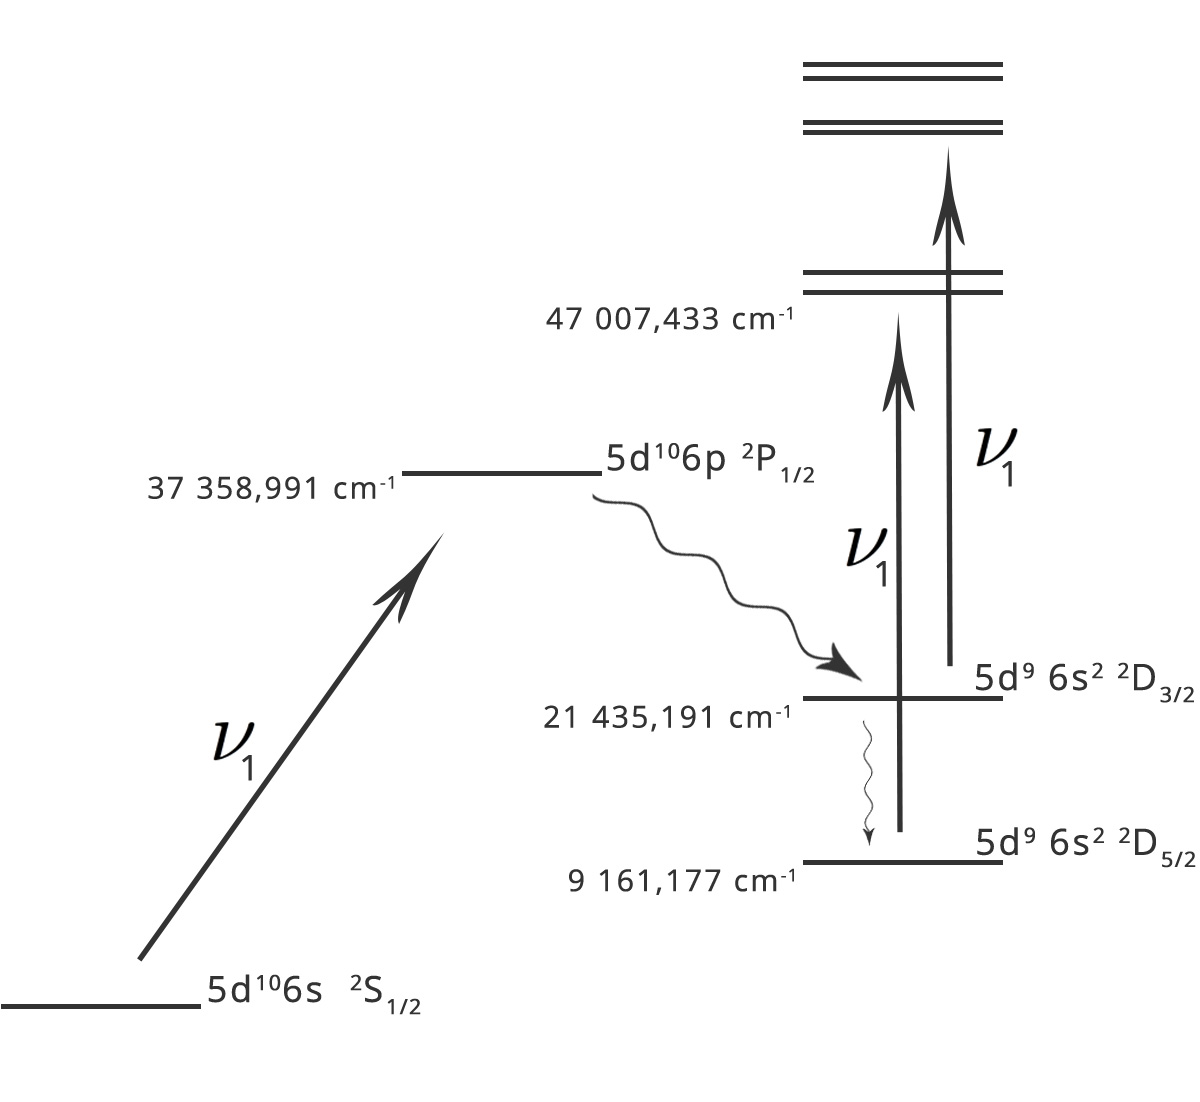
\includegraphics[width=9cm]{./results/au_trans.jpg}}
\captionabove{\label{autransall} \textsl{Gotrian diagram showing the relaxation from the $^2P^o_{1/2}$ state into the meta-stable D-states with spiral arrows. $\nu_1$ illustrates resonant excitations. Note that the relaxation $5d^9 6s^2 \ ^2D_{3/2} \rightarrow 5d^9 6s^2 \ ^2D_{5/2}$ is forbidden. }}
\end{figure}
This observation indicates that the atom in the droplet relaxed into the $^2D_{5/2}$ state (figure \ref{autransall}). Possible relaxation paths lead either via the allowed $^2P^o_{1/2} \rightarrow \ ^2D_{3/2}$ transition and subsequently the forbidden $^2D_{3/2} \rightarrow \ ^2D_{5/2}$ transition, or directly via the forbidden $^2P^o_{1/2} \rightarrow \ ^2D_{5/2}$ transition into the $^2D_{5/2}$ state. In both cases the transition is mediated and enhanced by the He$_N$ environment. The influence of the helium droplet can also be seen by comparing the theoretical and dimensionless transition probabilities f (''oscillator strength'') taken from ref. \cite{fivet}. For the $^2P^o_{1/2} \rightarrow \ ^2S_{1/2}$ transition f is 0.170 and for the $^2P^o_{1/2} \rightarrow \ ^2D_{3/2}$ transition f is 0.002, which means that for the free atom the transition into the $^2D_{3/2}$ state is two orders of magnitude weaker than the transition into the ground state. The time scale of the relaxation process has to be shorter than the $\unit[6.1]{ns}$ life time of the $^2P^o_{1/2}$ state. Considering the $\unit[28]{ns}$ pulse duration of the laser, a recycling process similar to Rb-He$_N$ (ref. \cite{aubock}) may also contribute to the efficient population of the meta-stable $^2D$ states. \\
From the $^2D_{5/2}$ state a second laser photon excites the atom into the $5d^9 6s 6p \ ^4P_{3/2}$ state and a third photon ionizes the atom.
%To observe the transition starting from the $^2D_{5/2}$ state the atom first has to be excited into the $^2P^o_{1/2}$ state. From this state the atom can relax into the allowed $^2D_{3/2}$ state. The helium droplet further enables the atom to relax into the $^2D_{5/2}$ state which would be forbidden otherwise. The relaxations are denoted with spiral arrows in figure \ref{autransall}. A second photon excites and a third photon ionizes the atom. \\

The fact that the spectrum in figure \ref{auspecfine} shows both, a sharp atomic and a blue shifted, broadened line suggests two processes after relaxation into the $^2D_{5/2}$ state: In one case the gold atom leaves the helium droplet resulting in a sharp line, which is a finger print of free atoms. In the second case the atom stays in the helium droplet resulting in the broadened, blue shifted line in the REMPI spectrum. The two processes are illustrated in figure \ref{twoprocesses}. For both cases a prior excitation into the $^2P^o_{1/2}$ state is necessary.

\begin{figure}[ht]
\centerline{
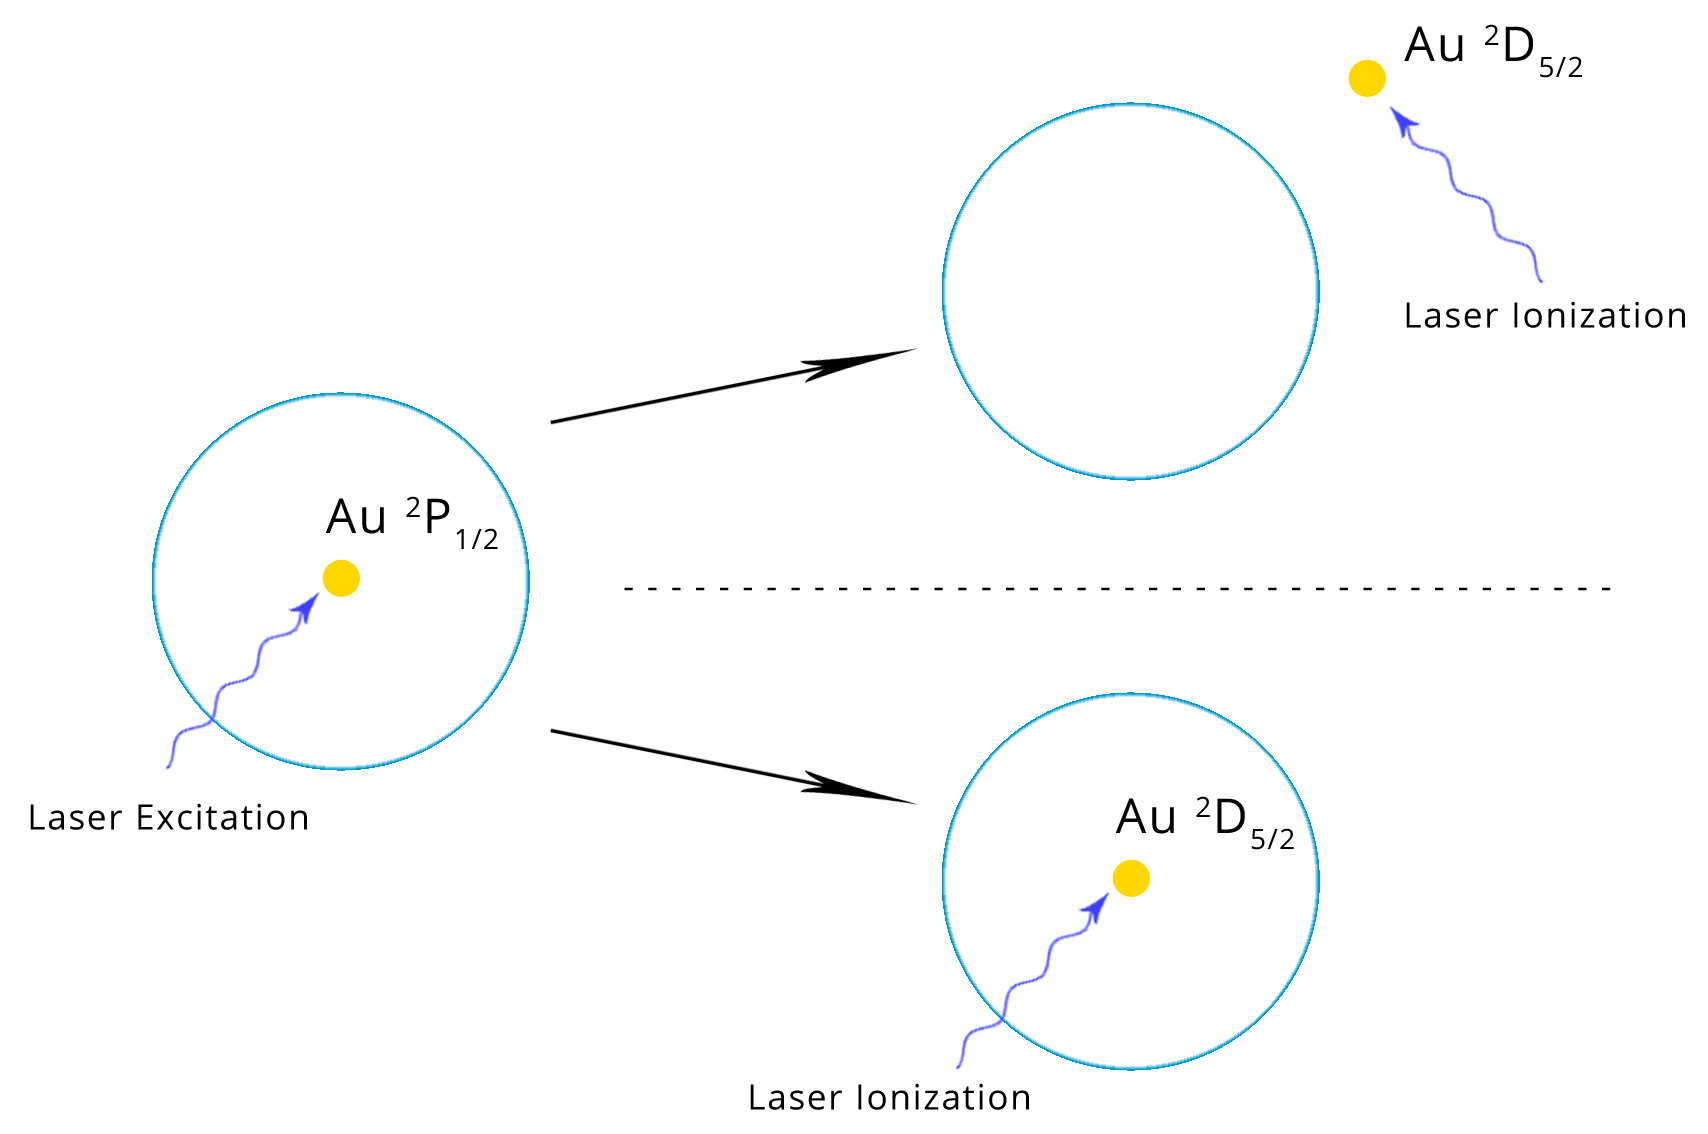
\includegraphics[width=9cm]{./results/Au_states.jpg}}
\captionabove{\label{twoprocesses} \textsl{a) The Au atom leaves the droplet after laser excitation. b) The Au atom remains in the droplet. The two cases lead to a sharp atomic line or a broadened, blue shifted structure, respectively.}}
\end{figure}

In addition to these two identified transitions, the spectrum shows several structures at energies above $\unit[39300]{cm^{-1}}$. This part of the spectrum is not sufficiently interpreted so far. The NIST database shows several levels with possible transitions in this wavelength range, originating from the two meta-stable $^2D$ states. Seven possible transitions in the wavelength range $\unit[37200-40000]{cm^{-1}}$ can be found in the NIST database (ref. \cite{nist}). Two of those transitions originate from the $^2D_{5/2}$ state and five from the $^2D_{3/2}$ state. The seven transitions are listed in table \ref{autransdenotation} and marked with black triangles in figure \ref{auspecalltrans}. %Note that figure \ref{auspecalltrans} additionally shows the ion yield for 4 x Au$_2$ (red) and 4 x Au$_3$ (blue).

\begin{table}[ht]
\small
%\centering
\captionabove{\textsl{Possible transitions within the spectral range of the Indigo-S laser ($\unit[37200-40000]{cm^{-1}}$) for the free Au atom with respective wavenumbers. The energies of upper and lower states can be obtained from the subtraction in the right column \cite{nist}. }}
\label{autransdenotation}
\begin{center}
% use packages: array
\begin{tabular}{c|c|c}

%\multicolumn{1}{c}{} & \multicolumn{1}{c}{From Pin number $\rightarrow$ to Pin number} & \multicolumn{1}{c}{} \\
Transition & energy difference [$cm^{-1}$] & line strength, \cite{nist} \\
\hline
\rowcolor{hellgrau}
$5d^96s6p \ ^4P^o_{3/2} \leftarrow 5d^{9} 6s^{2} \ ^2D_{5/2}$ & $47007,433 - 9161,177 = 37846,256$ & 250\\
\rowcolor{dunkelgrau}
$5d^96s6p \ ^4F^o_{9/2} \leftarrow 5d^{9} 6s^{2} \ ^2D_{5/2}$ &  $48697,147 - 9161,177 = 39535,97$ & n.a. \\
\rowcolor{hellgrau}
$5d^96s6p \ ^2P^o_{3/2} \leftarrow 5d^{9} 6s^{2} \ ^2D_{3/2}$ & $58845,414 - 21435,191 = 37410,223$ & n.a. \\
\rowcolor{dunkelgrau}
$5d^96s6p \ ^2F^o_{5/2} \leftarrow 5d^{9} 6s^{2} \ ^2D_{3/2}$ & $59713,2 - 21435,191 = 38278,009$ & n.a. \\
\rowcolor{hellgrau}
$5d^{10}7p \ ^2P^o_{1/2} \leftarrow 5d^{9} 6s^{2} \ ^2D_{3/2}$ & $60032,85 - 21435,191 = 38597,659$ & 30 \\
\rowcolor{dunkelgrau}
$5d^{10}7p \ ^2P^o_{3/2} \leftarrow 5d^{9} 6s^{2} \ ^2D_{3/2}$ & $60728,49 - 21435,191 = 39293,299$ & 16 \\
\rowcolor{hellgrau}
$5d^96s6p \ ^2D^o_{5/2} \leftarrow 5d^{9} 6s^{2} \ ^2D_{3/2}$ & $61255,1 - 21435,191 = 39819,909$ & n.a. \\
\end{tabular}
\end{center}
\end{table}

\begin{figure}[ht]
\centerline{
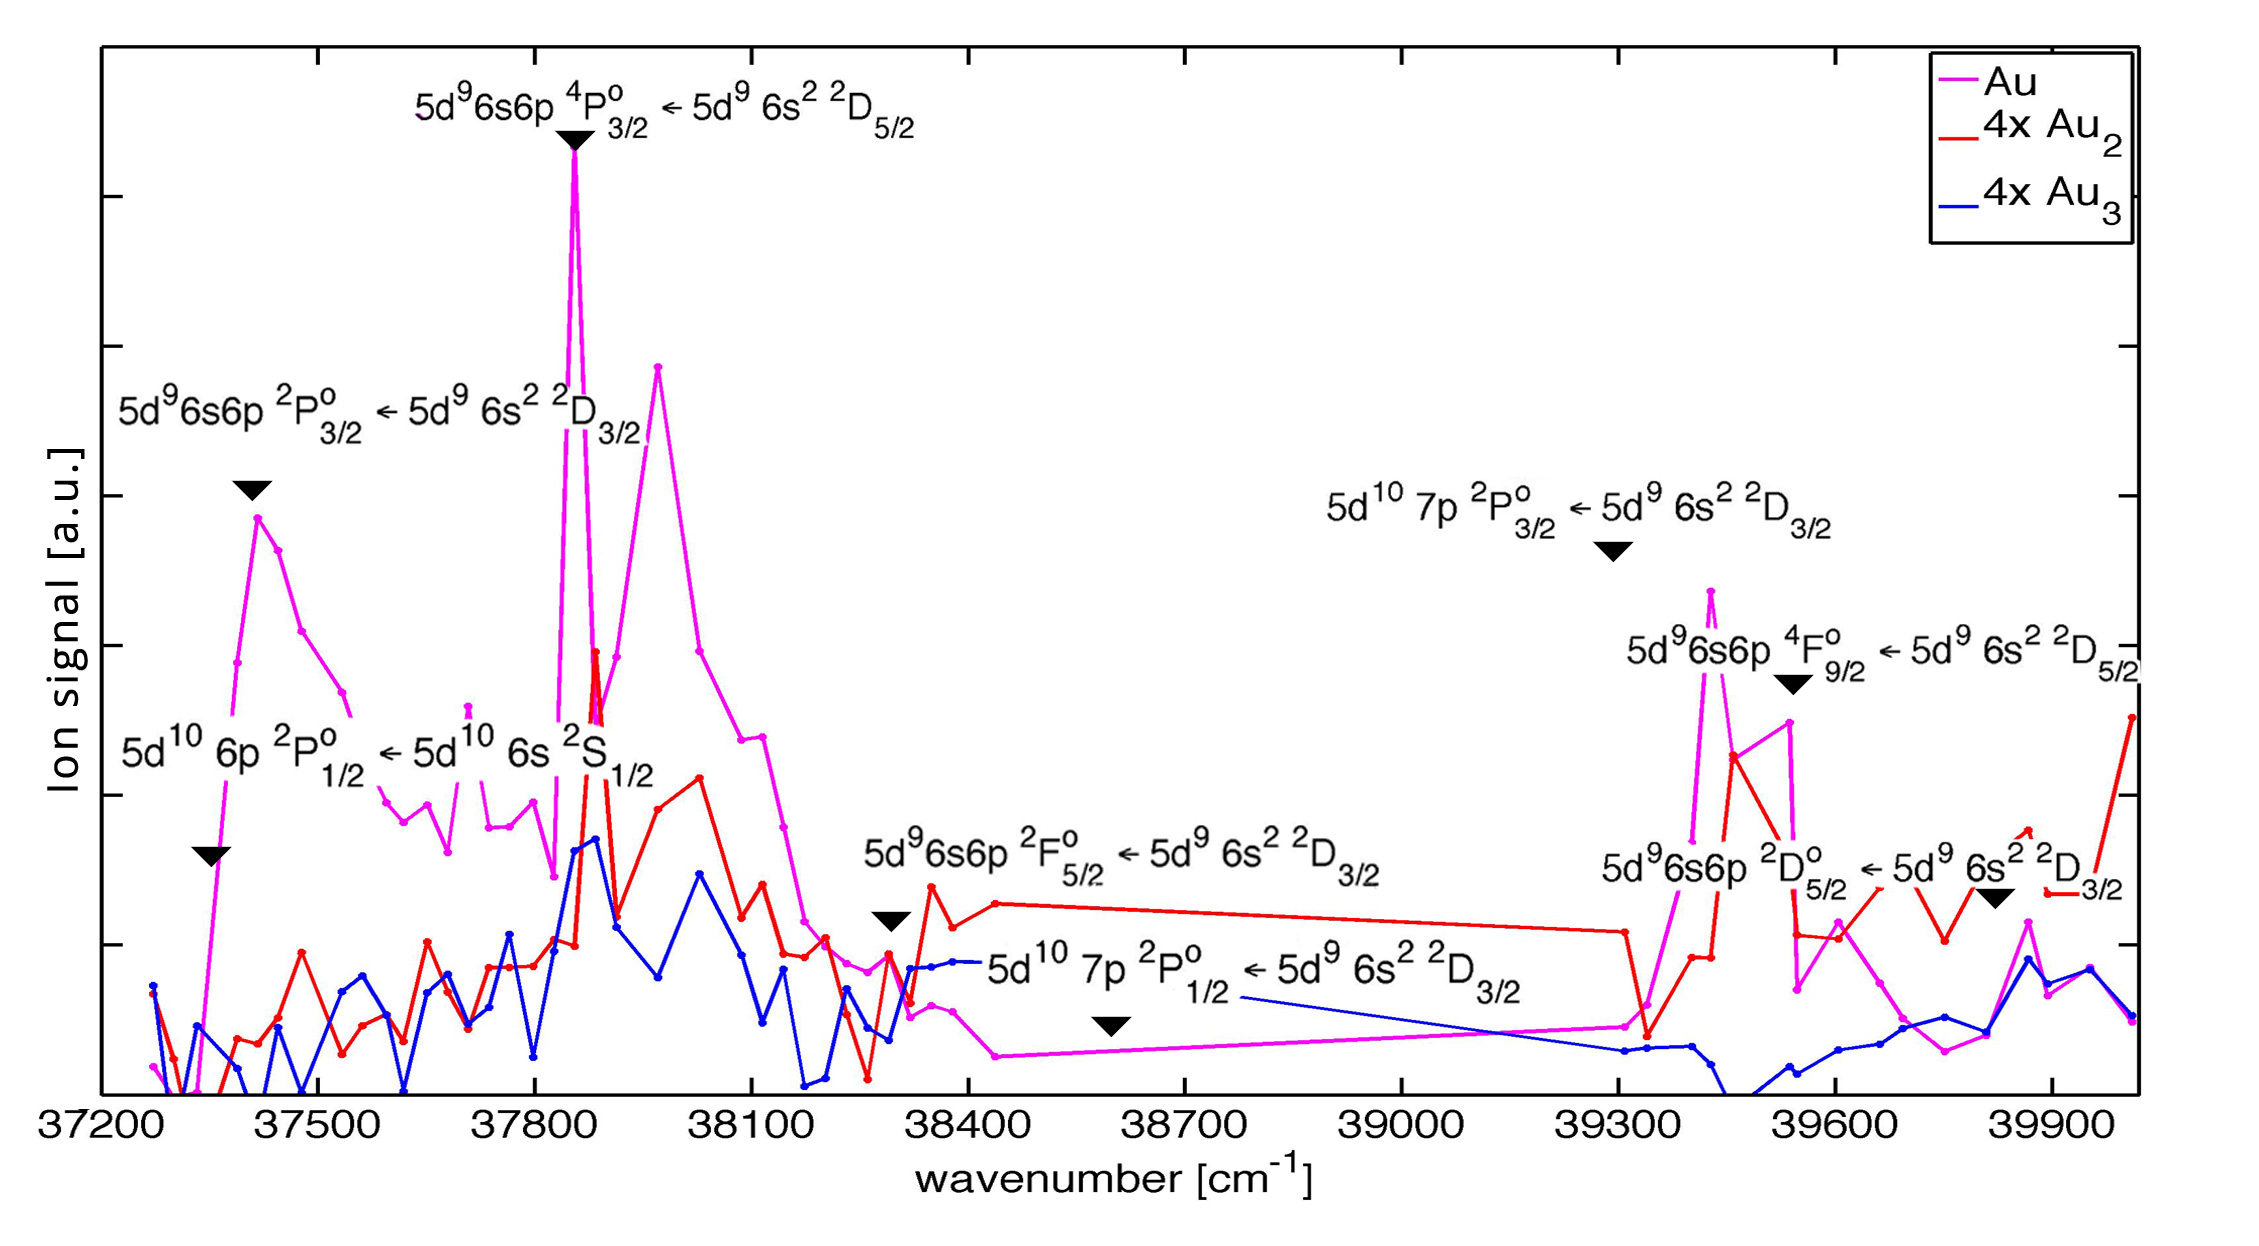
\includegraphics[width=16cm]{./results/au_spec_dimer.jpg}}
\captionabove{\label{auspecalltrans} \textsl{Spectrum of Au monomers, dimers and trimers. Transitions listed in table \ref{autransdenotation} are marked with a black triangle. }}
\end{figure}

\vspace{1cm}
\underline{Au dimers and trimers} \\
In addition to the ion yield for atoms, figure \ref{auspecalltrans} also shows the ion yield recorded for Au$_2$ and Au$_3$. It is remarkable that the signals for both molecules show a weak maximum at $\unit[37880]{cm^{-1}}$, approximately at the maximum of the peak which is associated with the atomic $5d^9 6s 6p \ ^4P^o_{3/2} \leftarrow 5d^9 6s^2 \ ^2D_{5/2}$ transition in the droplet. Similar observations have been reported in the history of HENDI spectroscopy, eg. K which follows Na$_2$ signals (ref. \cite{higgins}), Mg$_n$ (ref. \cite{mgn}) as well as Sr$_n$ (ref. \cite{bunermann-doc}). Possible explanations range from the formation of foam like structures, which collapse upon laser excitation to explanations based on the dissociation of molecules with subsequent surface migration and ion- atom/molecule recombination. \\
The fact that the molecule signal does not follow the initial $^2P^o_{1/2} \leftarrow \ ^2S_{1/2}$ transition suggests that the foam structure hypothesis is unlikely, because we do not expect that the foam structure survives the initial excitation and subsequent relaxation process into the $^2D_{5/2}$ state. \\
Although highly speculative, we favor another hypothesis which has been used as an explanation for unusual results in chromium experiments (ref. \cite{paperkautschkoch}). In this scenario it is assumed that the first photon dissociates a Au$_2$ or Au$_3$ molecule, resulting in a $^2D_{5/2}$ atom which is spatially separated from remaining ground state Au atoms or Au$_2$ molecules, respectively. A second photon can excite the separated $^2D_{5/2}$ atom, which is subsequently ionized by a third photon. The ion-neutral interaction differs from the neutral-neutral interaction in the helium droplet and the Au$^+$ ion may recombine with the remaining neutral Au or Au$_2$, thereby leading to a signal at the Au-He$_N$ $5d^9 6s 6p \ ^4P^o_{3/2} \leftarrow 5d^9 6s^2 \ ^2D_{5/2}$ transition.

\underline{Comparison with Cu and Ag} \\
As mentioned in the introduction of this chapter, spectroscopic data for the atoms Cu and Ag on helium nanodroplets are already available. Copper, silver and gold are in the same group of the periodic table and have similar electron configurations. All three elements have a single valence electron which makes them comparable to the alkali atoms. A comparison of the available spectra is therefore interesting and shown in figure \ref{cuagau}. The wavelength axis were scaled proportional. The three figures show REMPI spectra of the corresponding metals. \\
In all three spectra the lowest $^2P^o_{1/2} \leftarrow \ ^2S_{1/2}$ transition, marked with a gray line, can be seen at the left. The spectra for Cu and Ag show the two lowest atomic transitions $^2P^o_{1/2} \leftarrow \ ^2S_{1/2}$ and $^2P^o_{3/2} \leftarrow \ ^2S_{1/2}$. The fine structure splitting depends on the spin-orbit interaction which increases with the atomic number. For gold the $^2P^o_{3/2}$ state is not observable within the wavelength range accessible with the Indigo-S laser (the $^2P_{3/2}$ state is at $\unit[41 174.613]{cm^{-1}}$, resulting in a spin-orbit splitting of $\unit[3816]{cm^{-1}}$). For Ag the fine structure splitting of the $^2P$ level is with $\unit[921]{cm^{-1}}$ larger than for Cu with $\unit[248]{cm^{-1}}$.

\newpage

\begin{figure}[H]
\centerline{
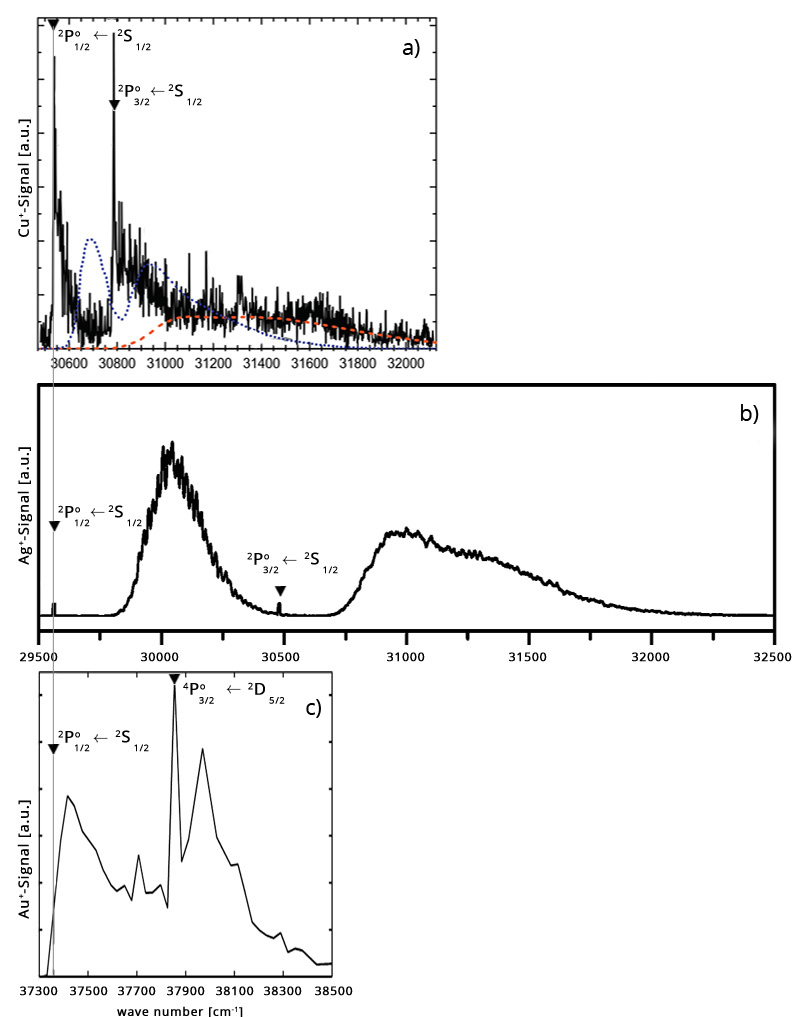
\includegraphics[width=12cm]{./results/Cu_Ag_Au.jpg}}
\captionabove{\label{cuagau} \textsl{Comparison of the three REMPI spectra for a) copper \cite{cufritz}, b) silver \cite{loginov2007excited} and c) gold. The gray line marks the lowest $^2P^o_{1/2} \leftarrow ^2S_{1/2}$ transition for all three elements. }}
\end{figure}

\newpage

\underline{Excitation spectra of Au and Ag doped He$_N$} \\
Prior to the Au experiments we tested the experimental setup with the Indigo-S laser and two subsequent ovens. One oven was loaded with Au (double basket setup) and the other oven was loaded with Ag (single basket setup). The goal of this test was to record the first REMPI spectra with the apparatus in Cluster Lab III. The same wavelength range as in the Au experiments was covered with the Indigo-S laser in $\unit[2]{nm}$ steps. Figure \ref{auag} shows the results of this test. The spectrum shows the ion yield for Au (yellow), Ag (blue), AuAg (cyan), AgHe (green), AgHe$_2$ (red), Ag$_2$ (magenta) and Ag$_3$ (black). Interestingly non-zero ion yields were measured for all masses except Ag$_3$.

\begin{figure}[ht]
\centerline{
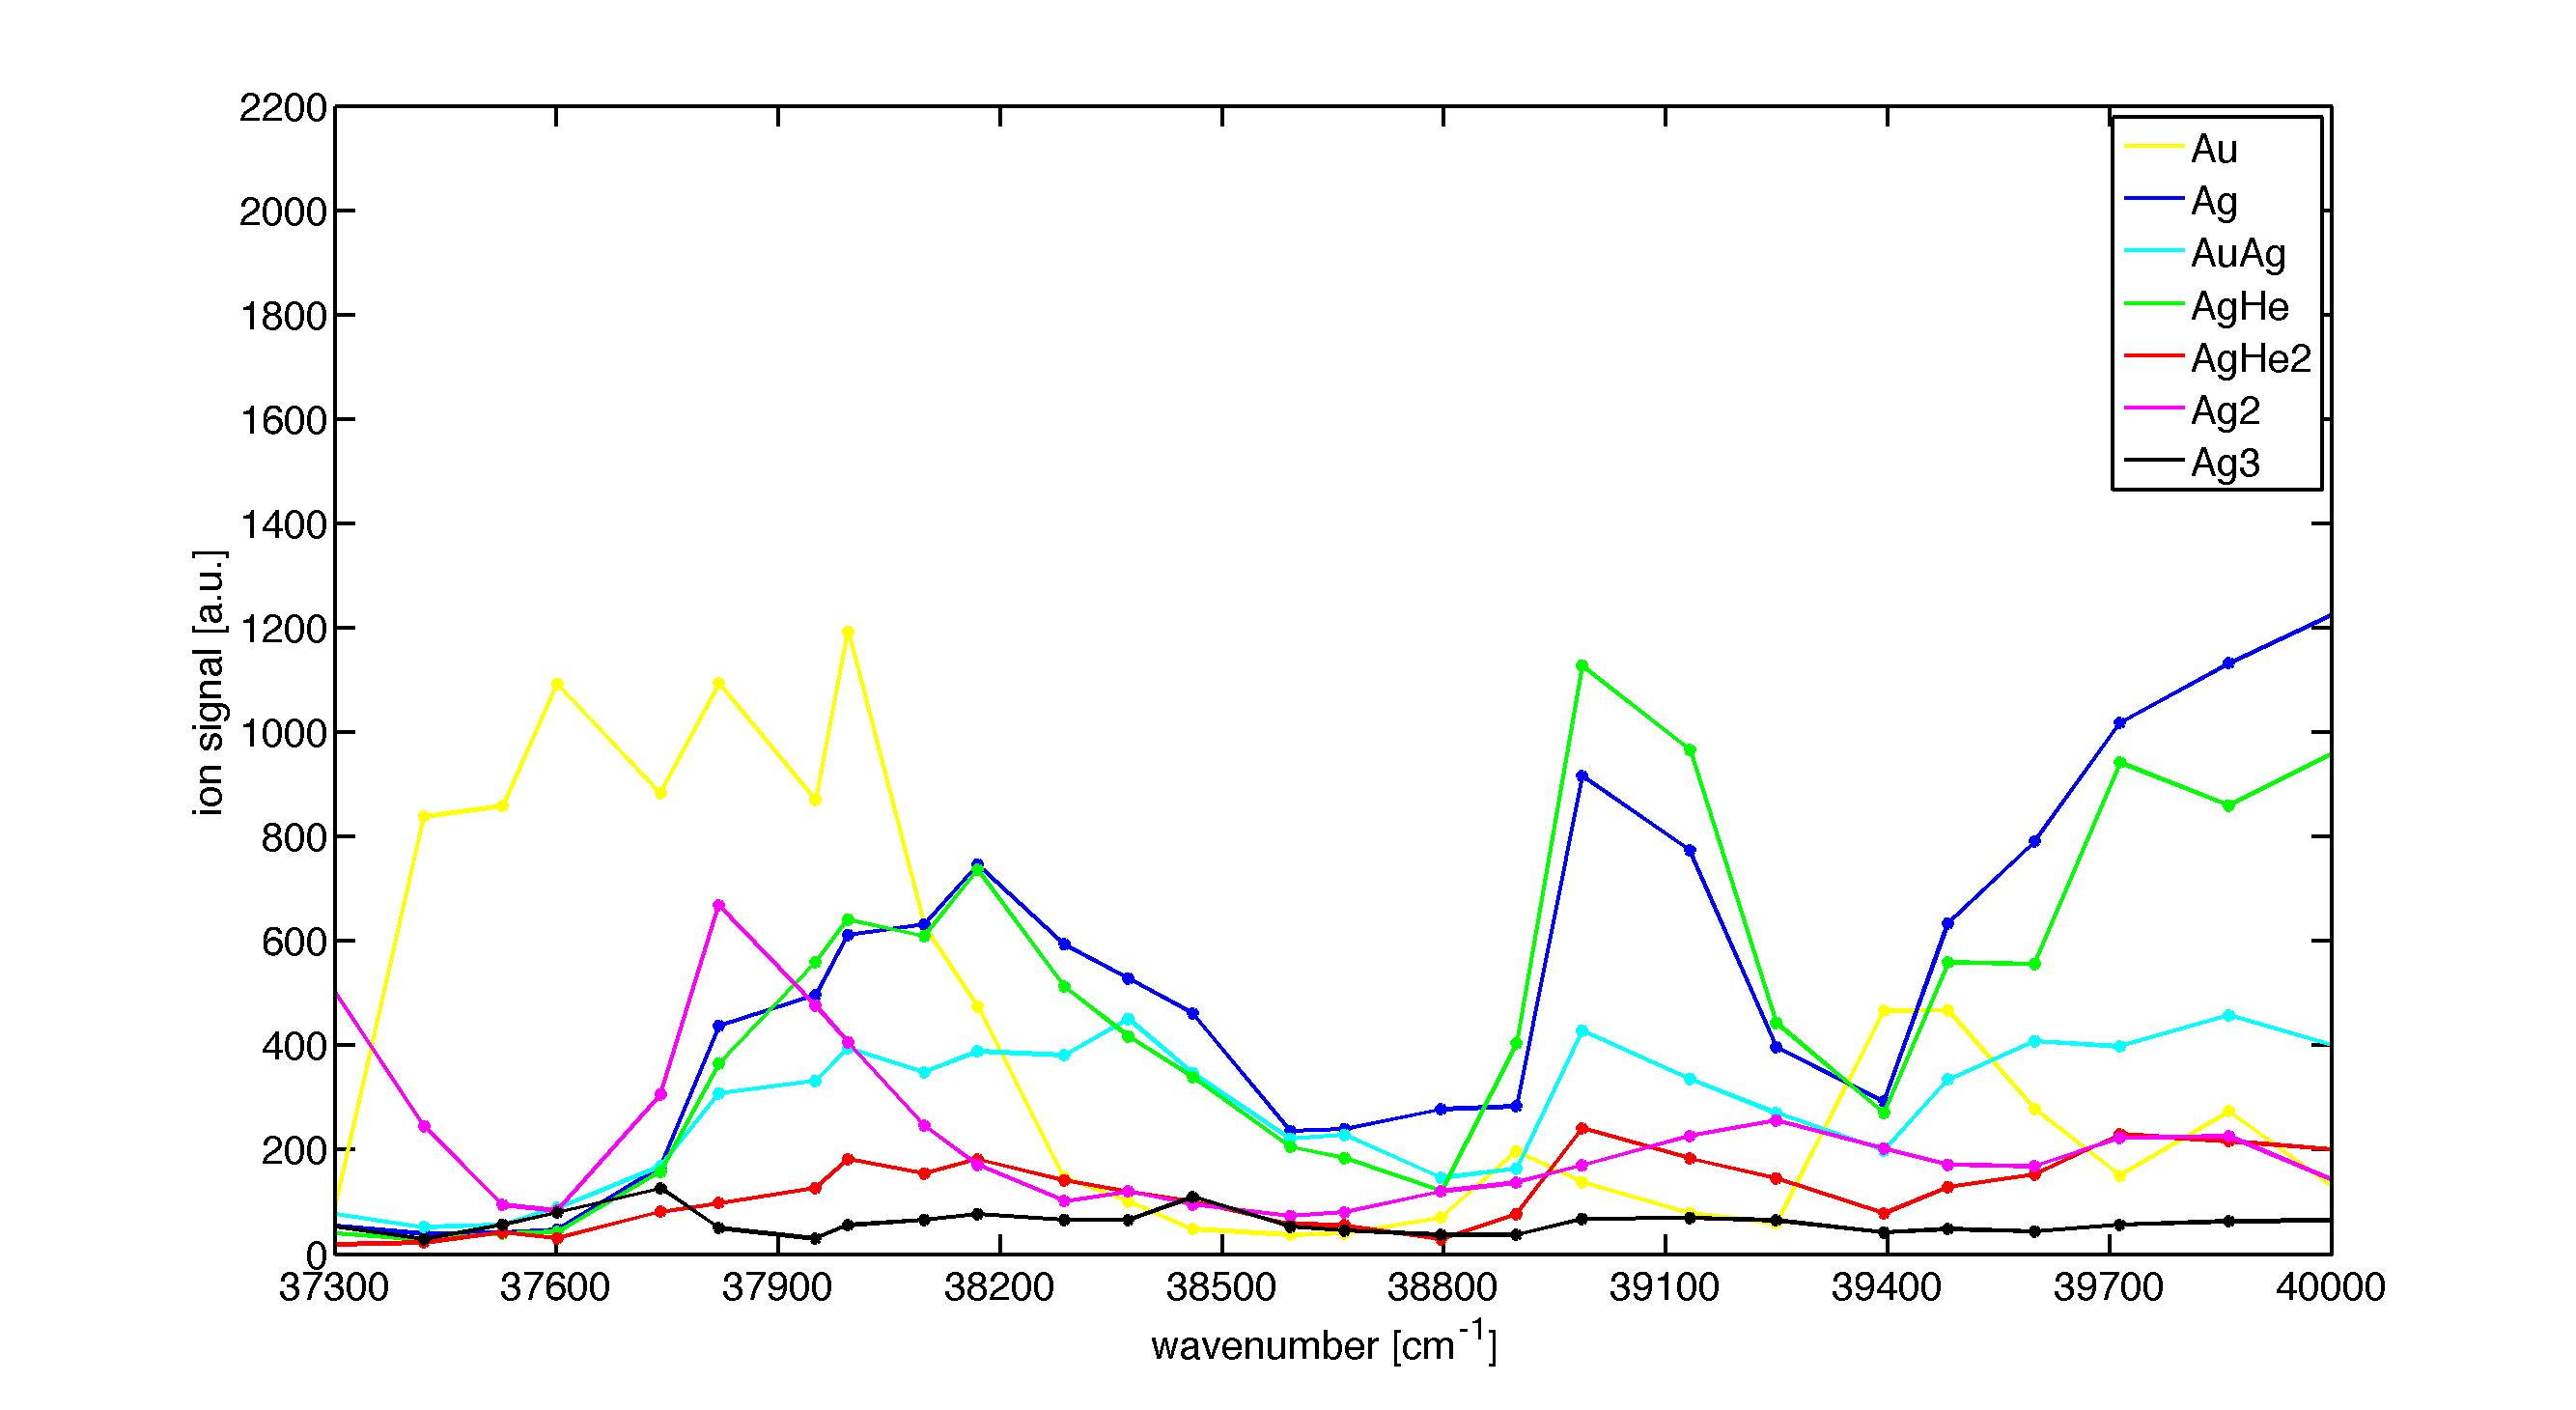
\includegraphics[width=19cm]{./results/au_ag_spec.jpg}}
\captionabove{\label{auag} \textsl{REMPI spectra obtained in a test with two subsequent ovens, one loaded with Au the other with Ag. The graphic shows the ion yield for Au (yellow), Ag (blue), AuAg (cyan), AgHe (green), AgHe$_2$ (red), Ag$_2$ (magenta) and Ag$_3$ (black). }}
\end{figure}


\chapter{High temperature pick up source for gold}
\label{chap:goldoven}
This chapter describes the pick up oven which was designed for high temperature metals and was used in the course of this thesis as a pick up source for Gold (Au). The main issues were the construction and implementation of the oven into the apparatus in Cluster Lab III as well as the direct temperature measurement of the liquefied metal. To install the high temperature oven in Cluster Lab I an aluminum frame was constructed. The mechanical drawings can be found in Appendix A. In addition a temperature controller was programmed in LabView which is described in detail in chapter \ref{chap:tempprogram}.

Temperatures higher than $\unit[1064]{^\circ C}$ (Au melting point) are needed in order to produce vapor pressures high enough for doping He$_N$ clusters with Au atoms. An aluminum coated tungsten wire basket (Ted Pella, basket style 6 \cite{albasket}) is used to evaporate the material. This basket allows to reach a maximum temperature of $\unit[1800]{^\circ C}$. According to the data sheet the temperature, which can be held over unlimited time periods, is limited to $\unit[1475]{^\circ C}$. The maximum heating current is $\unit[49]{A}$ with an overall heating power of $\unit[768]{W}$. Detailed informations about the basket can be found in ref. \cite{albasket}. \\

\section{The oven setup}
\vspace{-0.5\baselineskip}
The new oven design fits in all pick up chambers of our cluster laboratories at the Institute of Experimental Physics in Graz. It was designed by Phillip Thaler and fulfills some important requirements:
\begin{itemize}
%\item The oven can easily be adapted for all different pick up chambers in all laboratories.
\item The oven has a water cooled shield to minimize the influence of other ovens nearby.
\item The modular design allows to extend the pick up source with a second basket.
%\item Everything is build on top of a copper base plate which is water cooled as well.
\item It provides adaptable current connections on the bottom side of the base plate.
\end{itemize}

All gold experiments were done with the two-basket setup, shown in figure \ref{twobasket}, whereas silver experiments were performed with only one basket. In case of two baskets the second one is mounted flipped above the first one. The inner surfaces of the baskets face each other in this setup. Both baskets are then heated with the same current. In this way the second basket minimizes losses and confines the gold vapor within the volume of the two baskets. This is especially important for an expensive material like gold. Figure \ref{oven-one-basket-no-cooling} shows one basket with gold.

\begin{figure}[ht]
\centerline{
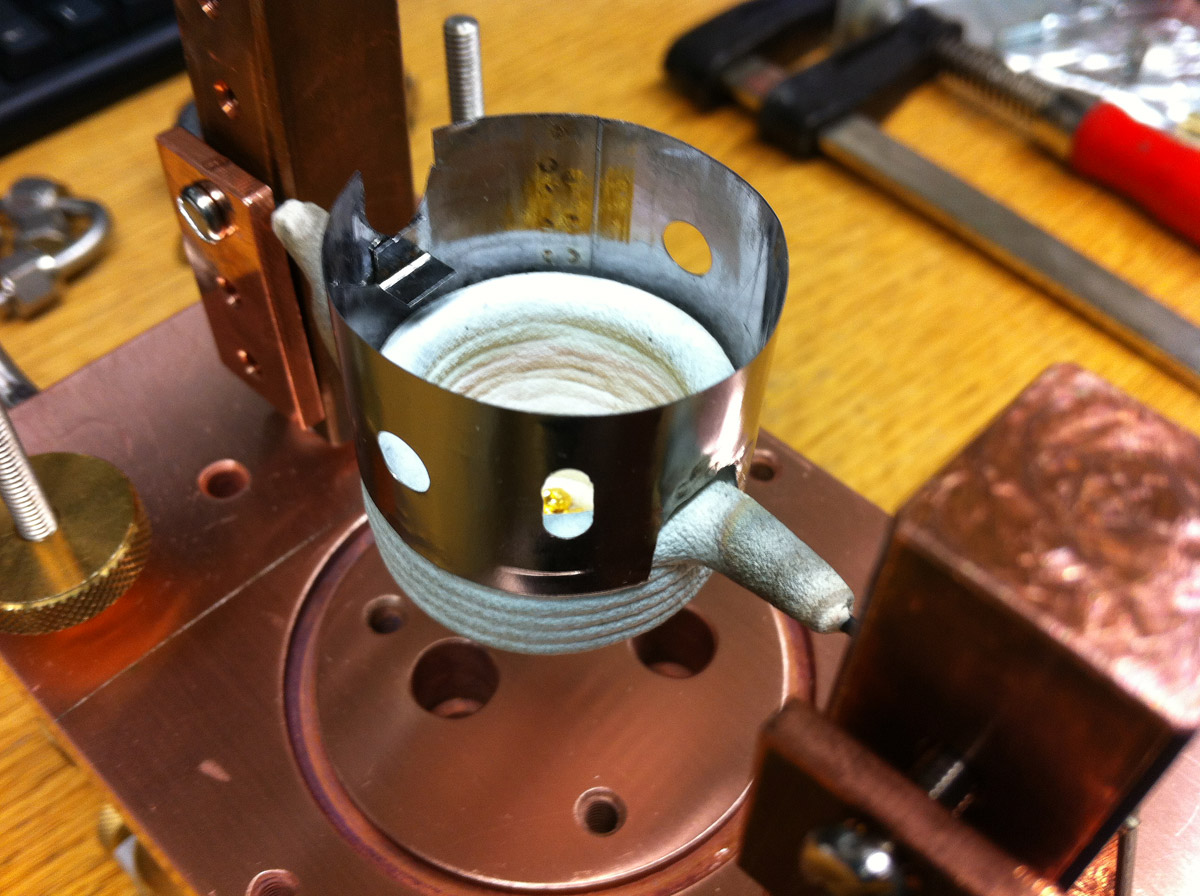
\includegraphics[width=10cm]{./oven/OneBasket_NoCoolingShield.jpg}}
\captionabove{\label{oven-one-basket-no-cooling} \textsl{Pick up source with the first basket filled with gold. The second oven is mounted flipped above the first one. The molybdenum ring provides an additional confinement for the gaseous metal. The whole setup is surrounded by a cooling shield in the final setup. }}
\end{figure}

\begin{figure}[ht]
\centerline{
\includegraphics[width=8cm]{./oven/twobasket.jpg}}
\captionabove{\label{twobasket} \textsl{Two-basket setup in the pick up chamber of the apparatus in Cluster Lab III. For illustration purposes without Molybdenum ring and cooling shield. }}
\end{figure}

The two centered circular holes in the molybdenum ring are the entry and exit holes for the helium droplet beam. The remaining third long hole is the feed through for the thermocouple. The fully assembled oven is shown in figure \ref{oven-assembled}.

\begin{figure}[ht]
\centerline{
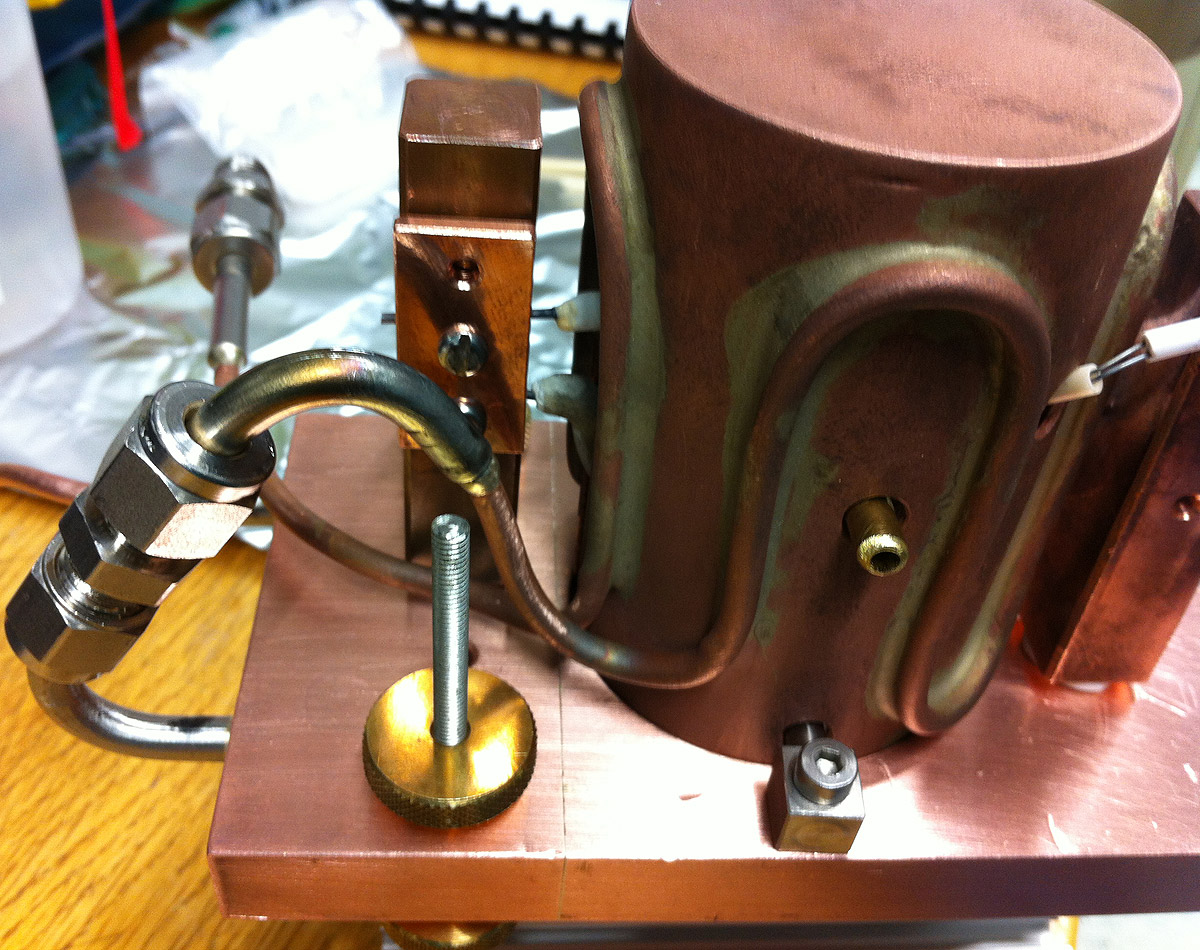
\includegraphics[width=10cm]{./oven/FullyAssembled.jpg}}
\captionabove{\label{oven-assembled} \textsl{Fully assembled gold oven with cooling shield and thermocouple. The connections for the water cooling are made of high quality steel for durability. The brass pipe to align entrance and exit holes is still in place. }}
\end{figure}


When assembling the oven one has to make sure that the entry and exit holes of the cooling shield, as well as those from the molybdenum ring are aligned properly. For this purpose a small brass pipe with the diameter of the entry and exit holes was used. It turned out that this pipe is also a great help to keep everything in place while the gold source is installed in the pick up chamber of the apparatus.

\section{Temperature measurement}
\vspace{-1\baselineskip}
Temperature measurements can quickly become complicated when measuring high temperatures of liquefied materials. In the past, conventional methods for the determination of the dopant temperature were based on indirect measurements of the pick up cell, not the liquid itself. In addition those methods did not offer the possibility to log and control the temperature via a computer. Both problems were solved during this thesis. \\


\subsection{Mounting the thermocouple}
\vspace{-1\baselineskip}
To measure the temperature with a thermocouple, one has to make sure that the only connection of the two thermocouple wires is at the point were the temperature should be measured. This means that the wires have to be protected from the vapor pressure within the pick up source. Evaporated metal condenses on the thermocouple wires and causes short-circuits. As a consequence the temperature is measured at the point where the two thermocouple wires are connected through the condensed metal. For our experiments the problem was solved with a ceramic tube ($\unit[3]{mm}$ diameter) with only one open end. This tube dips with the closed end into the liquid metal, shielding the thermocouple inside the tube from the liquid and the vapor on the outside of the tube. It is essential that the tube protects the thermocouple wires until they reach the feed through of the water cooled copper shield (figure \ref{oven-assembled}). \\
To make sure that the wires inside the tube are not connected, a separator was made out of a conventional isolation element. The isolation element was grinded until it was small enough to fit into the ceramic tube (together with the thermocouple).

The high temperatures in the gold experiments make it necessary to use type C thermocouples instead of type K. Temperatures of up to $\unit[2000]{^\circ C}$ can be measured with this type. More informations about type C thermocouples can be found in the data sheet which is available in ref. \cite{ref-typec}. \\


\subsection{Connecting the thermocouple with a Computer}
\vspace{-1\baselineskip}
Once the thermocouple is in place and the oven is installed in the pick up chamber, one can connect the thermocouple wires with the feed through on the inside of the pick up chamber. The outside of the feed through is connected directly with the Voltcraft Datalogger K204 which is used to measure the thermo voltage. The data sheet for the Datalogger can be found in ref. \cite{ref-datalogger}. \\
%Because the Datalogger is not able to measure thermo voltages of type C thermocouples the LabView program have to recal
%Originally the Datalogger K204 is not able to measure thermo voltages of type C thermocouples. It is only calibrated for the use with conventional type K thermocouples. This problem is solved with recalculating the voltage via the LabView program and is explained in more detail in chapter \ref{chap:tempprogram}. \\
Although the Datalogger can be directly connected with a computer, it is not recommended. The temperature measurements are known to be unreliable in this case. To prevent this, the Datalogger is connected with an optocoupler which sends the data to the computer. The reason for the unreliable measurements are most likely unwanted ground connections between the ports of the Datalogger.

The next step is to connect computer and power supply to control the heating current and therefore the temperature.

\subsection{Connecting the power supply}
\vspace{-1\baselineskip}
The power supply (Elektroautomatik PS9000), used to supply the heating current for the oven, offers a parallel port for remote control. The manufacturer provides a sample LabView program to communicate with the device. To connect computer and power supply, a parallel-USB adapter, also available from Elektroautomatik, is needed (UTA12 interface, ref. \cite{ref-uta12}). While the UTA12 is directly connected with the computer via USB, a customized parallel cable is used to connect the UTA12 with the parallel port of the power supply. A data sheet with the pin assignments of this cable is available on the website of Elektroautomatik \cite{ref-uta12}. The pin assignment, which actually works, is not identical with the one listed in the data sheet. The working pin assignment developed during a trial and error process is listed in table \ref{wireing}. Figure \ref{adapter-pins} shows the connectors schematically in order to define the pin numbers. The connectors are drawn from the back side. The parallel connector is male, the serial is a female.

\begin{figure}[ht]
\centerline{
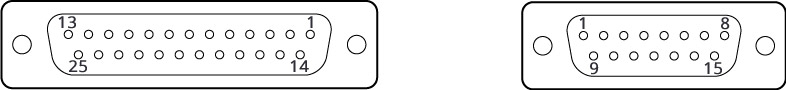
\includegraphics[width=13cm]{./oven/DSub.jpg}}
\captionabove{\label{adapter-pins} \textsl{Parallel (left) and serial (right) connectors viewed from the back side. }}
\end{figure}
\begin{table}[h]
%\centering
\captionabove{\textsl{Adapter to connect the serial port from UTA12 with the parallel port of the power supply. ''P'' specifies the pin number of the parallel port, ''S'' the number on the serial port.}}
\label{wireing}
\begin{center}
% use packages: array
\begin{tabular}{c|c|c}
\multicolumn{1}{c}{} & \multicolumn{1}{c}{From Pin number $\rightarrow$ to Pin number} & \multicolumn{1}{c}{} \\
\hline
\rowcolor{hellgrau}
1P $\rightarrow$ 18P & 11P $\rightarrow$ 13S & 21P $\rightarrow$ 23P \\
\rowcolor{dunkelgrau}
2P $\rightarrow$ 2S & 12P $\rightarrow$ 15S & 22P $\rightarrow$ 5S \\
\rowcolor{hellgrau}
3P $\rightarrow$ 1S & 13P $\rightarrow$ 7S & 23P $\rightarrow$ 21P \\
\rowcolor{dunkelgrau}
4P EMPTY & 14P EMPTY & 24P EMPTY \\
\rowcolor{hellgrau}
5P $\rightarrow$ 9S & 15P $\rightarrow$ 4S & 25P EMPTY \\
\rowcolor{dunkelgrau}
6P $\rightarrow$ 10S & 16P EMPTY & 20P $\rightarrow$ 11S \\
\rowcolor{hellgrau}
7P EMPTY & 17P EMPTY & 10P $\rightarrow$ 8S \\
\rowcolor{dunkelgrau}
8P $\rightarrow$ 14S & 18P $\rightarrow$ 1P & 19P EMPTY \\
\rowcolor{hellgrau}
9P $\rightarrow$ 6S &  &  \\
\end{tabular}
\end{center}
\end{table}


\chapter{Programming a temperature controller in LabView}
\label{chap:tempprogram}
This chapter describes the LabView program which controls the heating current of the oven. In previous experiments the oven temperature was controlled by an external PID temperature controller (Eurotherm). Although this setup is well tested, the temperature can not be logged via PC. The LabView block diagram is documented in the following.

\section{Requirements}
\label{chap:requirements}
\vspace{-0.5\baselineskip}
In our first approach we controlled the temperature of the basket via setting a specific current (at constant voltage). It turned out that this procedure does not lead to reproducible results. Every time the basket was heated up, the same pairs of current and voltage resulted in different temperatures. \\
Figure \ref{prob-basket-heating} shows a test, where the basket was heated up to more than $\unit[1100]{^\circ C}$ , held constant at the corresponding voltage/current pair for about 5 minutes and cooled down to $\unit[800]{^\circ C}$. Note that the graph in figure \ref{prob-basket-heating} was obtained with a type K thermocouple and an empty basket. The results are also quantitatively valid for type C thermocouples. \\
The figure illustrates both, positive and negative properties of this method. The basket temperature responds linearly to the power, which is an advantage. One of the biggest problems can be seen at the maximum temperature. At that point current and voltage were held constant for about 5 minutes, but this didn't result in a constant temperature. The temperature decreased by about $\unit[30]{^\circ C}$ without changing current or voltage. During experiments this behavior is unacceptable.
The attempt to reach a specific point on the heating curve via cool down failed also. The resulting temperature was about $\unit[30]{^\circ C}$ lower than during the previous heating phase. \\
Therefore, temperature controlling via setting the heating power, is not sufficient. In fact we figured out that it is much better to measure the actual basket temperature and hold it constant by regulating the heating current (at constant voltages). A simple controller which heats when the temperature is lower than the desired temperature and switches the power supply off when the temperature is too high gives a relatively high jitter ( $\pm \unit[40]{^\circ C}$). Tests showed, that reproducible results with low jitter are only possible with a PID controller (Proportional-Integral-Derivative controller). A PID controller calculates an error value from the difference between the measured temperature and the desired temperature. The error value is minimized by adjusting the heating current.


\begin{figure}[ht]
\centerline{
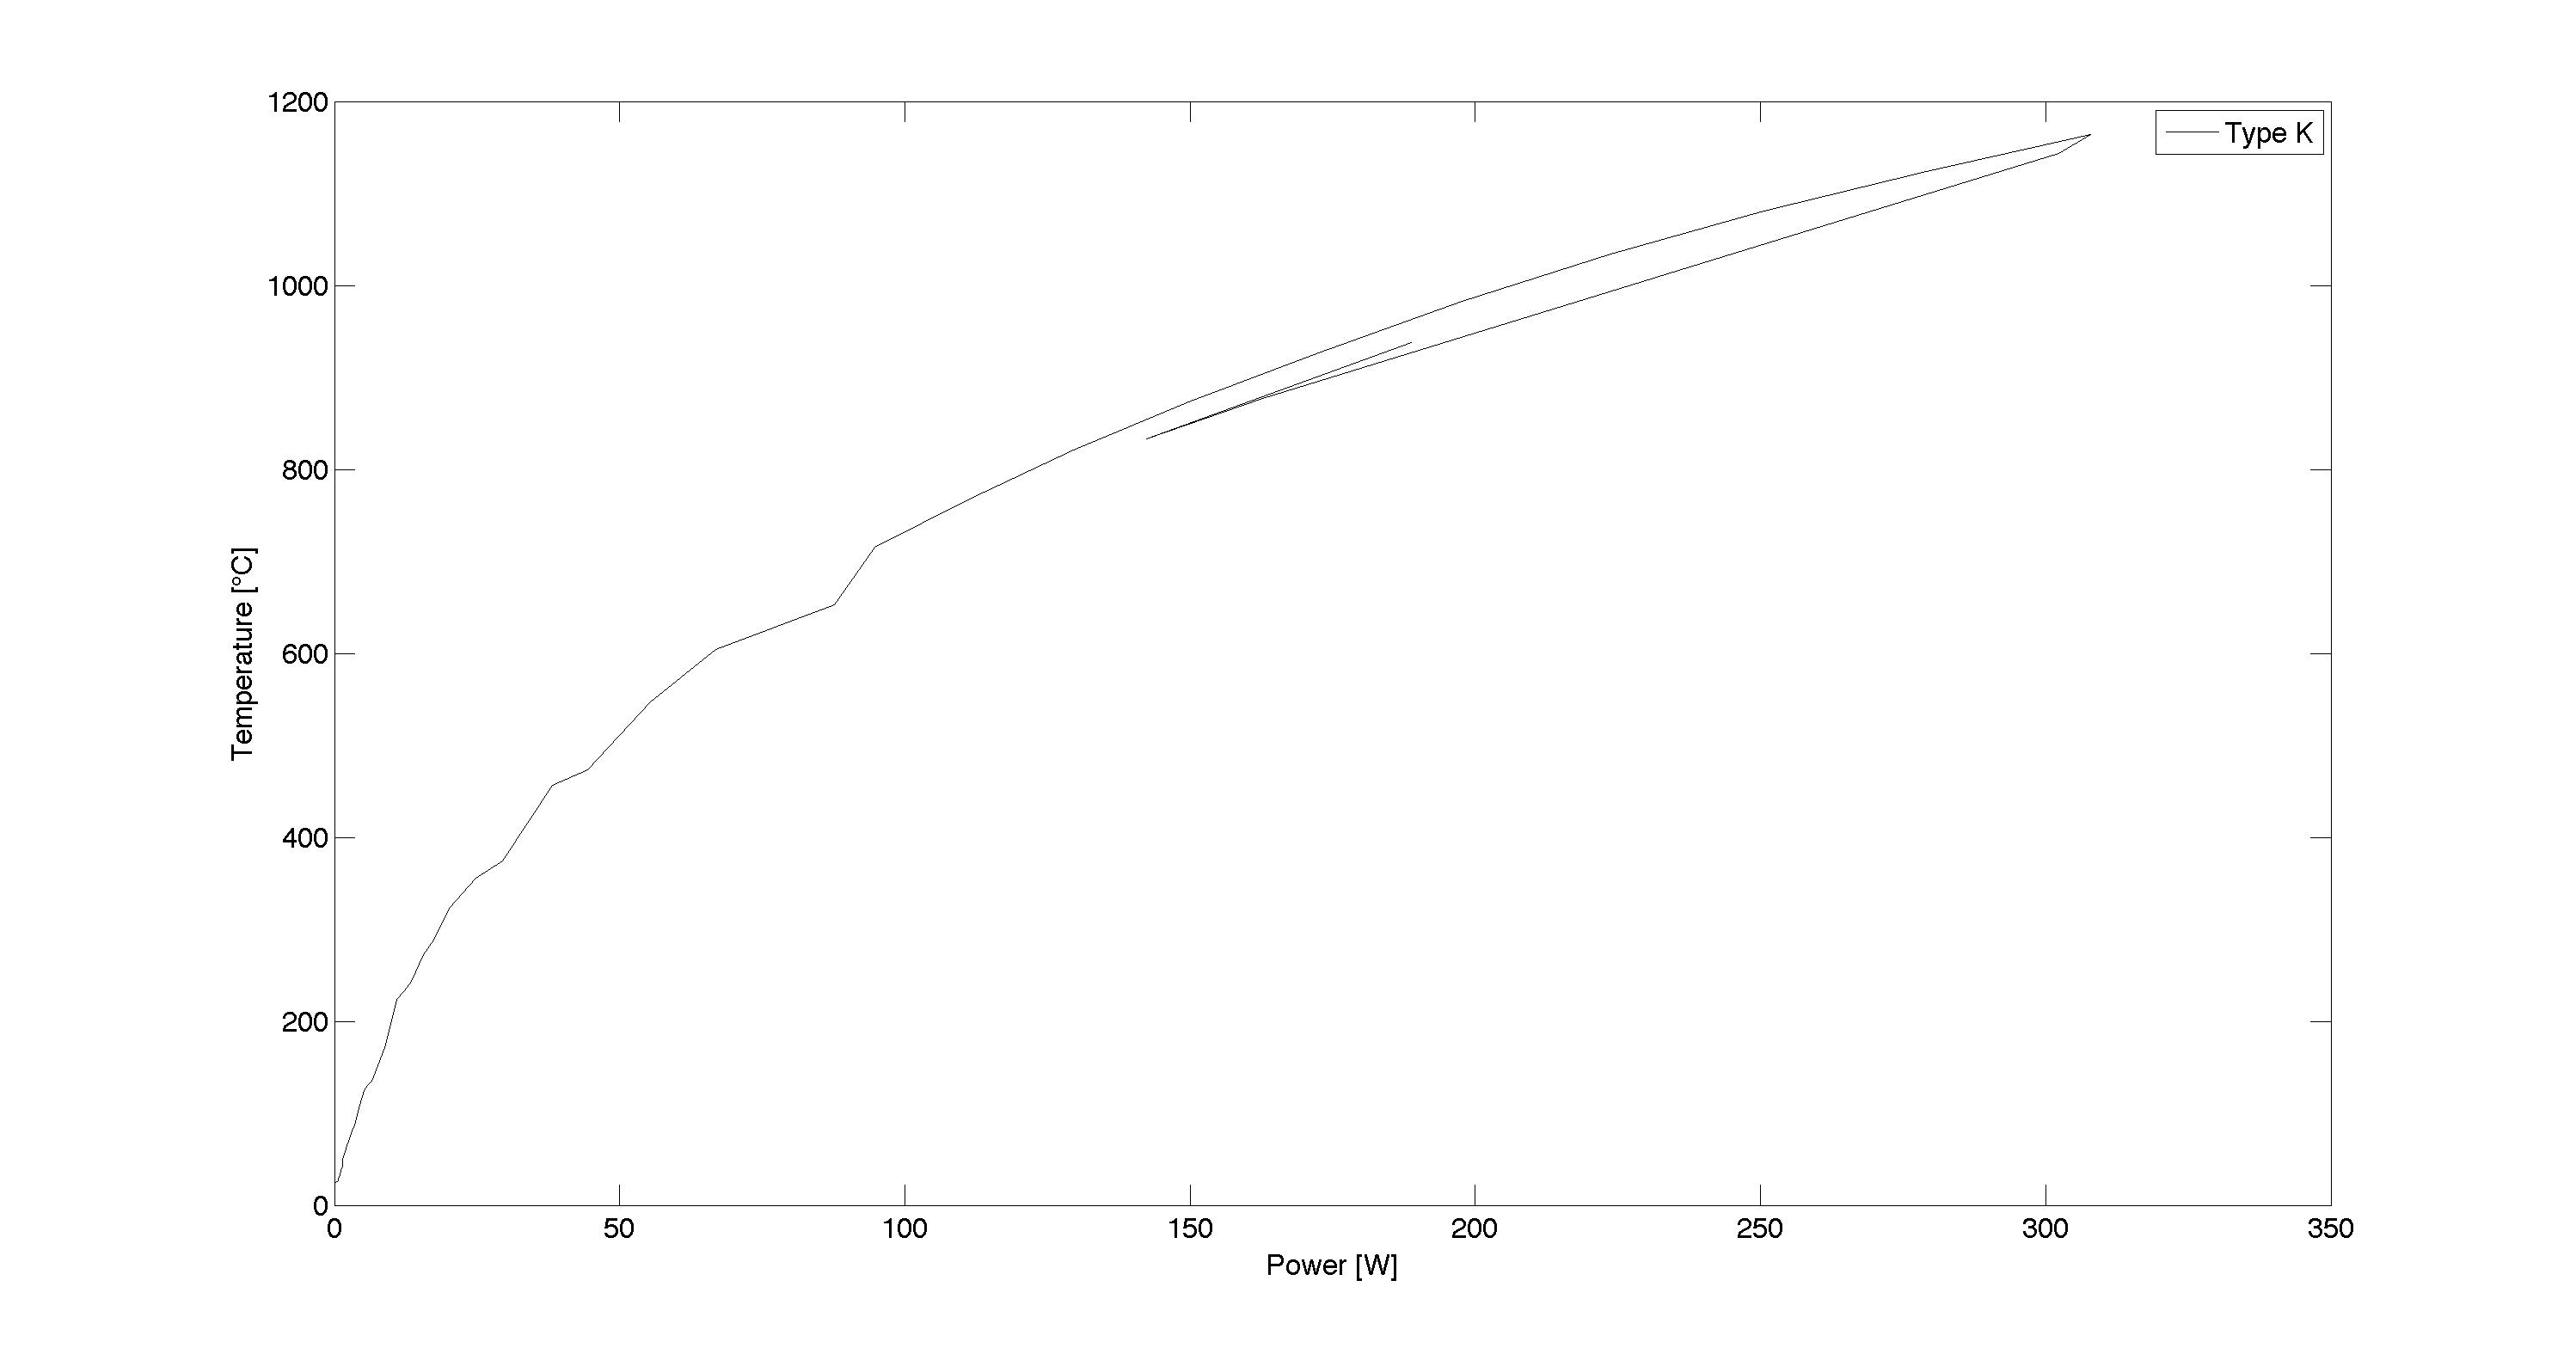
\includegraphics[width=18cm]{./temperature/01072013_HeatUpDown.jpg}}
\captionabove{\label{prob-basket-heating} \textsl{Problems during basket heating tests. The graph shows three phases: the heat up phase to about $\unit[1150]{^\circ C}$, a phase were current and voltage were held constant and the cool down to about $\unit[800]{^\circ C}$ with subsequent heat up to $\unit[900]{^\circ C}$.}}
\end{figure}

After these tests, the required features of the LabView program were defined as follows:

\begin{itemize}
\item The program should control the current of an external power supply. The voltage is not preset, it obeys ohm's law.
\item The measured temperature should be displayed. Because a conventional Voltcraft Datalogger K204 is used, which natively only supports type K thermocouples, the LabView program has to recalculate the temperature for type C accordingly.
\item A software PID controller (provided by the LabView program package) should regulate the heating current, appropriate PID parameters have to be found.
\item The basket must not undergo fast temperature changes at temperatures lower than $\unit[300]{^\circ C}$. The LabView program should be able to warm up the basket with a temperature gradient lower than $\unit[4]{^\circ C}$ per minute. The same applies to the cool down process.
\item The program should be able to handle one- and two-basket setups.
\end{itemize}

The LabView block diagram of the final program is documented in the following.

\section{Documentation of the LabView block diagram}
\vspace{-0.5\baselineskip}
%The first problem to solve was the connection with the power supply Elektroautomatik PS9000. The manufacturer of the device already shipped a working LabView program for this task \cite{ea-downloads}. The whole LabView temperature controller is based on this communication program.
The LabView program is divided into three main parts identifiable through the three sequences (0, 1, 2) of the stacked sequence structure (film strip) in figure \ref{labview-block}. Sequence 0 scans available power supplies and lists them in a drop down menu. Sequence 1 is responsible for establishing a communication with the power supply and for the calculation of temperatures and currents. Sequence 2 closes the connection to the power supply. Sequences 0 and 2 of the template were no changed. For more informations relating to this parts have a look at the data sheet provided by Elektroautomatik \cite{ref-ps}. Further explanations in this section only refer to sequence 1.

\begin{figure}[ht]
\centerline{
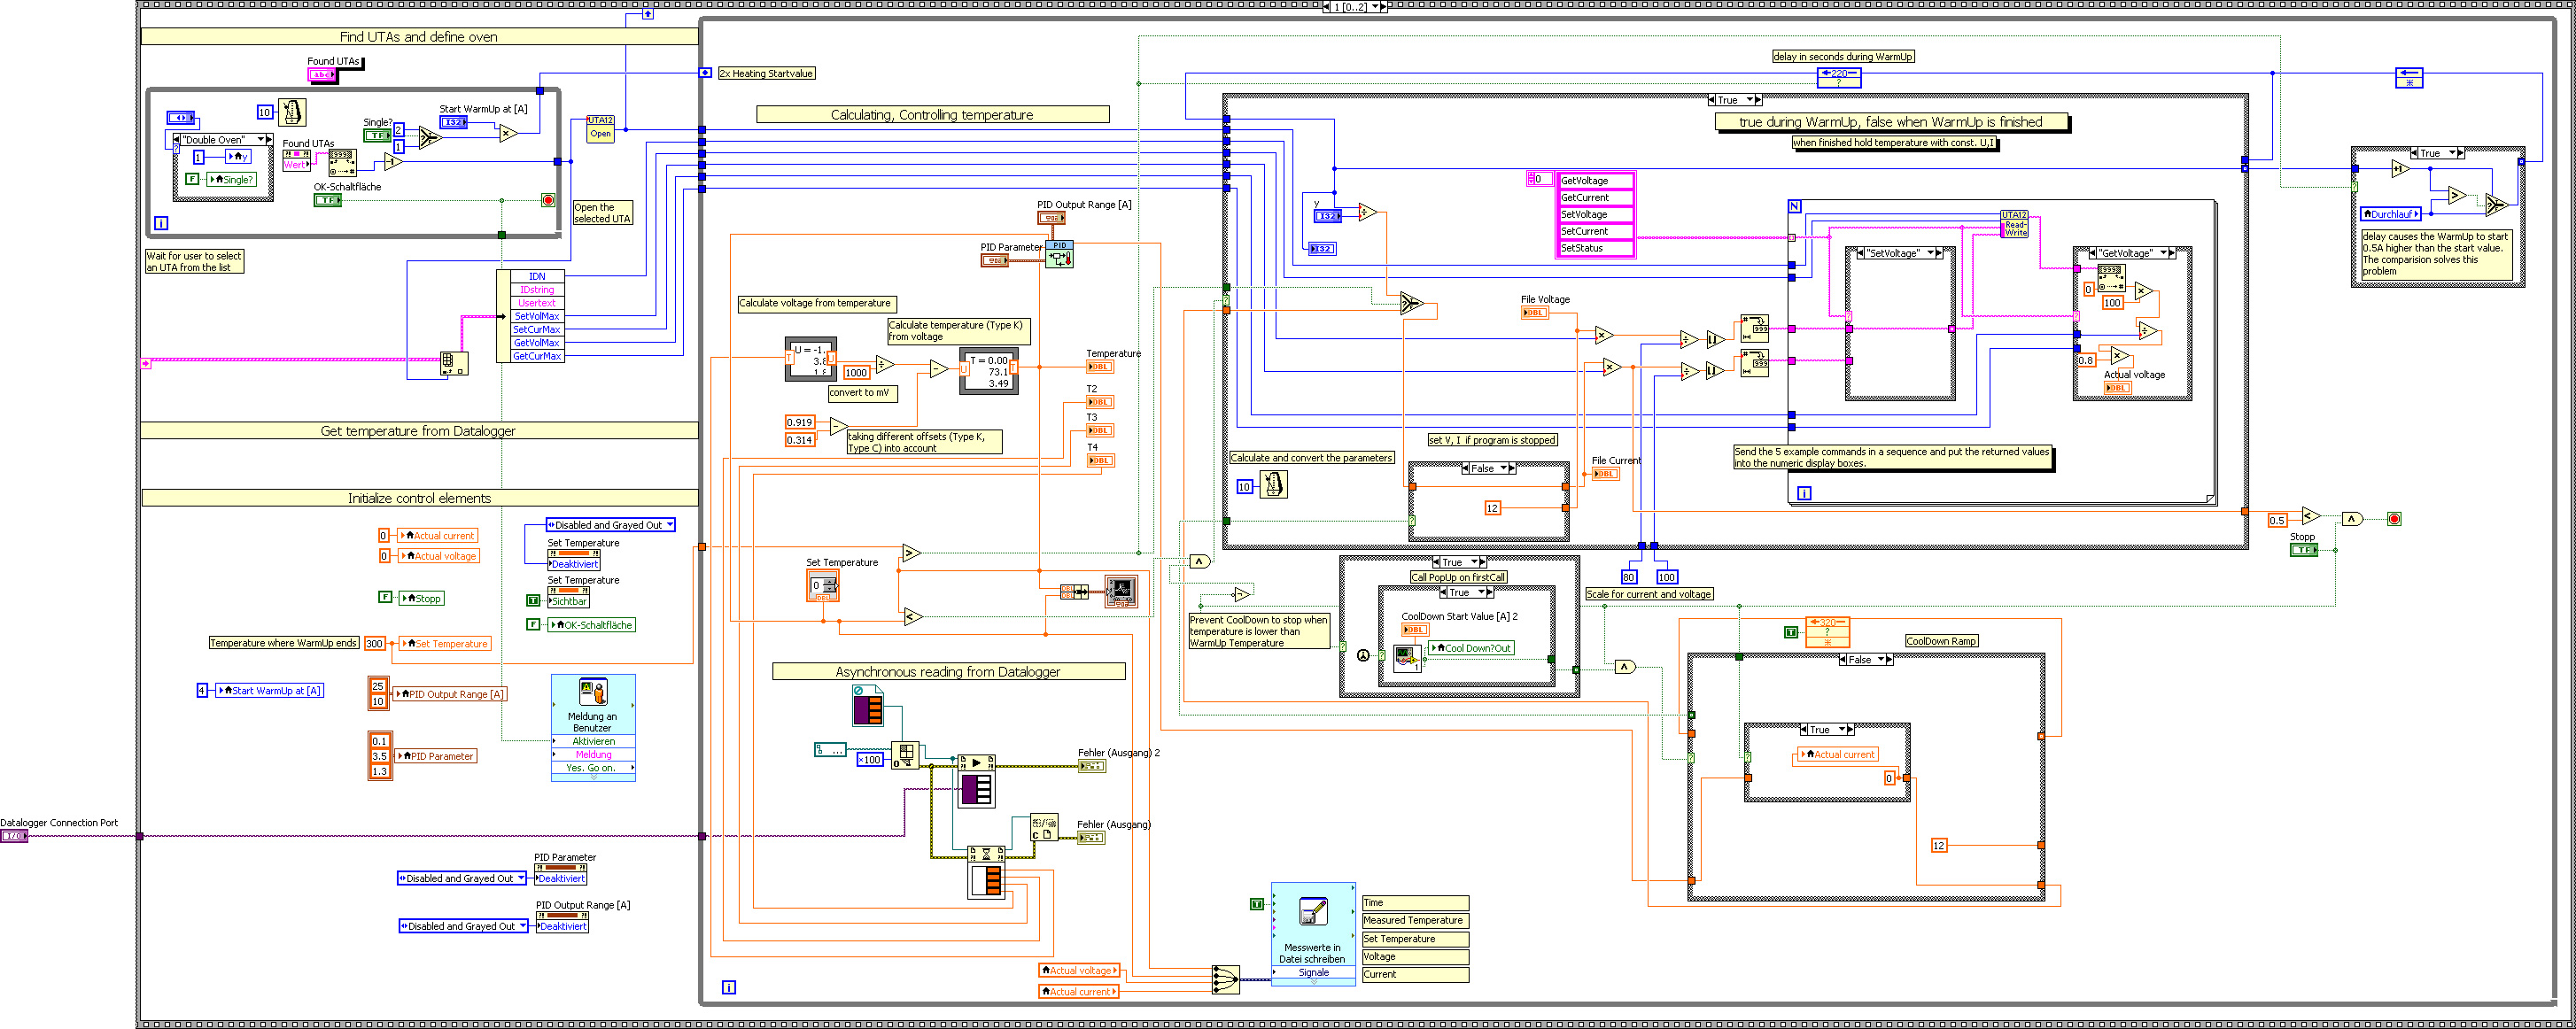
\includegraphics[width=16cm]{./labview/overview.jpg}}
\captionabove{\label{labview-block} \textsl{Block diagram of the final LabView program. The stacked sequence structure (film strip) is the outermost frame. }}
\end{figure}

All important parts of the program are labeled with yellow description tags for documentation. The parts ''Find UTAs'' and the for-loop in the large, outermost case-structure are from the original power supply communication program. The rest was added in order to establish the required additional functions listed in section \ref{chap:requirements}. The following sub sections correspond to the yellow description tags in the block diagram, figure \ref{labview-block}.

\subsection{Initialize control elements}
\vspace{-1\baselineskip}
The first task of the program is, to initialize control elements and variables. This is done immediately after the program is started, because otherwise it would be possible to start with high heating currents from a previous experiment. The PID parameters ($P = 0.1$, $I = 0.01$, $D = 0.3$), the output range and the warm up temperature are set automatically. An exception is the start current for the warm up. Due to the communication with the power supply the current has to be set within the while case, labeled as ''Find UTAs and define oven''. \\
When the program has successfully started the user can adjust the setting for starting current, oven type, used power supply and communication port for the Datalogger in the front panel, shown in figure \ref{labview-front}.


\subsection{Asynchronous reading from the Datalogger}
\vspace{-1\baselineskip}
The section ''Asynchronous reading from Datalogger'' in the block diagram is responsible for reading the temperature from the Datalogger. The block loads an external vi (saved as ''K204 Display.vi'') which establishes the connection. The basic functionality of this vi was programed by Friedrich Lindebner. Tests showed that it is necessary to integrate this vi asynchronously, because otherwise temperature values are not read. In this case the LabView temperature controller gets ''NAN'' instead of a real temperature value. The reason for this failure is most likely the different reading cycles of power supply and Datalogger. A good explanation of asynchronous reading in LabView can be found in the LabView help section under ''Asynchronously Calling VIs''.

\subsection{Converting the thermal voltage}
\vspace{-1\baselineskip}
Once the type K temperature is available in the program, it can be converted into the equivalent type C temperature. This is done in two steps. First of all, the type K temperature is transformed into the corresponding type K thermal voltage using the direct polynomials from the thermocouple manufacturer Omega \cite{omega-polynomials}. For converting type K temperatures above $\unit[0]{^\circ C}$ the direct polynomial is

\begin{align}  \label{direct-polynomial}
U = \sum\limits_{i=0}^n c_i \cdot (t_{90})^i + \alpha_0 \cdot \exp(\alpha_1 \cdot (t_{90} - 126.9686)^2)
\end{align}

All coefficients $c_0$...$c_9$ as well as both constants $\alpha_0$ and $\alpha_1$ are listed on the Omega website \cite{omega-polynomials}.

In LabView the formula is implemented as

\begin{multline}  \label{implemented-polynomial}
U = -1.7600413686 \cdot 10 + 1.185976 \cdot 10^2 \cdot exp(-1.183432 \cdot 10^-4 \cdot (T-126.9686)^2) + \\
    3.8921204975 \cdot 10 \cdot T + 1.185976 \cdot 10^2 \cdot exp(-1.183432 \cdot 10^-4 \cdot (T-126.9686)^2) + \\
    \quad \,\,\,1.8558770032 \cdot 10^-2 \cdot T^2 + 1.185976 \cdot 10^2 \cdot exp(-1.183432 \cdot 10^-4 \cdot (T-126.9686)^2) - \\
    \quad \,\,\,9.9457592874 \cdot 10^-5 \cdot T^3 + 1.185976 \cdot 10^2 \cdot exp(-1.183432 \cdot 10^-4 \cdot (T-126.9686)^2) + \\
    \quad \,\,\,3.1840945719 \cdot 10^-7 \cdot T^4 + 1.185976 \cdot 10^2 \cdot exp(-1.183432 \cdot 10^-4 \cdot (T-126.9686)^2) - \\
    \quad \quad5.6072844889 \cdot 10^-10 \cdot T^5 + 1.185976 \cdot 10^2 \cdot exp(-1.183432 \cdot 10^-4 \cdot (T-126.9686)^2) + \\
    \quad \quad5.6075059059 \cdot 10^-13 \cdot T^6 + 1.185976 \cdot 10^2 \cdot exp(-1.183432 \cdot 10^-4 \cdot (T-126.9686)^2) - \\
    \quad \quad3.2020720003 \cdot 10^-16 \cdot T^7 + 1.185976 \cdot 10^2 \cdot exp(-1.183432 \cdot 10^-4 \cdot (T-126.9686)^2) + \\
    \quad \quad9.7151147152 \cdot 10^-20 \cdot T^8 + 1.185976 \cdot 10^2 \cdot exp(-1.183432 \cdot 10^-4 \cdot (T-126.9686)^2) - \\
    \quad \,1.2104721275 \cdot 10^-23 \cdot T^9 + 1.185976 \cdot 10^2 \cdot exp(-1.183432 \cdot 10^-4 \cdot (T-126.9686)^2) \\
\end{multline}

After obtaining the corresponding voltage, one has to take the offset between type K and type C measurements into account. This offset results from the fact that type K and type C supply different voltages at room temperature ($\unit[23]{^\circ C}$). Voltages and their respective temperatures of type C and type K thermocouples can be obtained from the Omega reference tables in ref. \cite{ref-typec} and \cite{ref-typek}. According to these tables the type C supplies $\unit[0.314]{mV}$ whereas the type K supplies $\unit[0.919]{mV}$ at room temperature. This offset is subtracted in the LabView block diagram.

For the second step, the transformation of the type K voltage into type C temperature, one needs the recursive polynomial. Unfortunately the data sheet (ref. \cite{omega-polynomials}) does not list polynomials for type C thermocouples. Therefore the polynomial was obtained by manually fitting the type C thermocouple characteristic from the reference table in \cite{ref-typec}. For the LabView calculation the following polynomial was used (obtained from the fit):

\begin{multline}  \label{fit-polynomial}
T = 0.00036607033979 + 73.15121202 \cdot U - 3.4901476382 \cdot U^2 + 0.2973265406 \cdot U^3 - \\
    0.014640523567 \cdot U^4 + 0.00039799817557 \cdot U^5 - 0.0000043837094235 \cdot U^6 \\
\end{multline}

After these calculations the Datalogger temperature for a type K thermocouple is transformed into the respective type C temperature. The results are in very good agreement with type C measurements of an Eurotherm temperature controller.

\subsection{PID temperature controlling}
\vspace{-1\baselineskip}
The PID controller is a ready-to-run vi from the LabView PID Toolkit. For this program the ''PID Autotuning (Temperature)'' controller was used. Detailed informations about this vi can be found in the LabView documentation under ''PID Autotuning (Temperature) VI''. \\
In this implementation only three inputs are used:

\begin{itemize}
\item The temperature input. This input supplies the measured and recalculated type C temperature value.
\item PID output range. This enables the user to set minimum and maximum heating current.
\item The P-I-D parameter input fields to manually enter the P, I and D parameters of the controller.
\end{itemize}

The P, I and D parameters as well as the PID output range can be adjusted via the front panel (figure \ref{labview-front}). The PID parameters depend on the temperature and were determined empirically. Good start values are $P = 0.1$, $I = 0.01$ and $D = 0.3$. \\
The minimum and maximum current values were also determined during tests. With $\unit[35]{A}$ one can heat up the single-basket setup to $\unit[1100]{^\circ C}$.

The only output of the PID controller is the heating current which is directly sent to the power supply. %The last thing happening before sending is scaling the values to match the output range of the power supply ($\unit[80]{A}$ and $\unit[100]{V}$).

\subsection{Warm up and conventional operation mode}
\vspace{-1\baselineskip}
There are three different cases in which the program behaves differently. The warm up phase, the conventional operation mode and the cool down. The first two cases correspond directly to the large case-structure within the while loop (figure \ref{labview-block}). The true case handles the warm up phase and the false case contains the functionality for normal operation mode. In this two true/false cases most of the functionality is related to the communication with the power supply. Every block is labeled according to its function (for example ''Get Current'', ''Set Current'',...).

The warm up mode has to increase the heating current slowly to prevent damage of the basket due to thermal strain. The current is increased in $\unit[0.5]{A}$ steps in single oven mode and in $\unit[1]{A}$ steps in double oven mode. By default the time delay between two steps is set to 250 seconds. In LabView this task is done by using a shift register with a callback value. The callback value corresponds to the next current value being set. The logic checks if the actual temperature of the basket is lower than the warm up temperature set at program start. The default warm up temperature is $\unit[300]{^\circ C}$ and can be changed manually in the block diagram (section ''Initialize control elements''). If the actual temperature is lower than the warm up temperature the program enters the true case and increases the current via the shift resister subsequently every 250 seconds. It stops the warm up when the temperature gets higher than the warm up temperature. Then the false case comes into play. This case is independent from the shift register. It does not heat the basket with the callback value. Instead it heats it with the current determined by the PID controller. Note that the front panel control element ''Set Temperature'' is not set active during warm up. This control element is deactivated when initialized, to prevent the user presetting any temperatures during warm up.

The callback value for the warm up process has to pass a true/false case-structure before it gets to the time delay. In the LabView block diagram one can find this structure rightmost within the while loop. Without this case-structure the warm up does not start with the set start value. It would begin $\unit[0.5]{A}$ higher. In general a starting value of $\unit[4]{A}$ is recommended, because below this value the temperature only rises very slowly.

\subsection{Cool down}
\vspace{-1\baselineskip}
The cool down phase serves the same purpose as the warm up - preventing the basket from thermal strain. The critical temperature range is $\unit[300 - 23]{^\circ C}$. The cool down is an optional procedure which can be manually started from a pop up windows when the user stops the program. Beginning from a starting value, entered by the user, the cool down decreases the current successively until $\unit[0.5]{A}$ are reached. \\
In the block diagram the functionality can be found right beneath the case structure for warm up/normal operation mode. There are two case structures, one handling the pop up behavior, one for calculating the cool down ramp. The cool down ramp has a higher delay between current steps - $320$ seconds per default. \\
Next to the stop button in the block diagram is the logic which terminates the cool down when the calculated current is lower than $\unit[0.5]{A}$.

\subsection{Frontpanel}
\vspace{-1\baselineskip}
The front panel, shown in figure \ref{labview-front}, enables the user to control process parameters and visualizes the current temperature in a diagram. After program start a power supply and the appropriate communication port for the Datalogger can be chosen from the drop down menus. Typically the COM port 6 is the one connected with the Datalogger. \\
After choosing from the drop down menus, one has to set the option for single- or double basket setup. Depending on the basket setup the recommended starting value for the warm up is $\unit[4]{A}$ (single basket) or $\unit[8]{A}$ (double basket).

If these 4 parameters are set, one can click ''Connect \& Warm Up''. A dialog pops up where the user has to confirm, that the water cooling is on. After that, the warm up starts automatically. For the next 90 minutes the warm up mode heats the basket up to a temperature of $\unit[300]{^\circ C}$. This is the default warm up temperature and can only be edited via the block diagram. There is no user control in the frontpanel to change this temperature.

During the warm up phase most control elements are disabled because the user is not meant to influence this phase. When the basket reaches more than $\unit[300]{^\circ C}$ the program activates all control elements and the user can set current, PID output range and PID parameters.

\begin{figure}[ht]
\centerline{
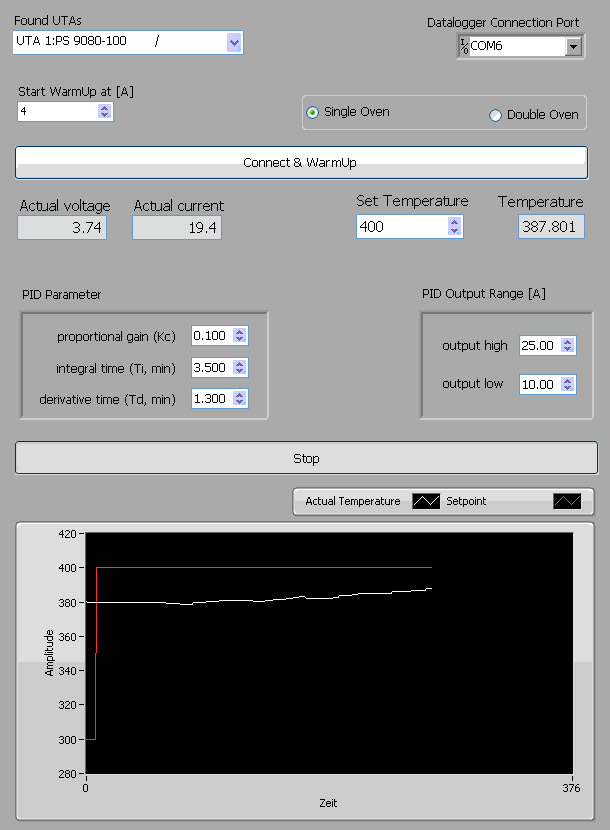
\includegraphics[width=10cm]{./labview/frontpanel.jpg}}
\captionabove{\label{labview-front} \textsl{Front panel to control process parameters and visualize the current temperature in the diagram. }}
\end{figure}

\subsection{Known issues}
\vspace{-1\baselineskip}
There are three known issues with the LabView program.

\begin{itemize}
\item The program does not check if all devices are connected correctly. Make sure to connect everything properly before starting the program. Otherwise irritating error messages might lead to time consuming troubleshooting.
\item Sometimes, even if everything is connected correctly, an error message ''No interfaces found...'' appears at the start of the application. In that case just try to close LabView and restart it again.
\item If someone stops the program manually the current may not be set to zero. In such a case the last value is still preset on the power supply. After stopping check the current manually before leaving the laboratory.
\end{itemize}

\chapter{Summary and Conclusion}
In the course of this thesis the RbSr molecule and the Au atom were investigated spectroscopically on and in helium nanodroplets, respectively. The spectra for RbSr were recorded with resonance enhanced multi-photon ionization (REMPI-TOF) as well as laser induced fluorescence (LIF) spectroscopy in Cluster Lab I. A REMPI overview spectrum in the wavelength range from $\unit[11600]{cm^{-1}}$ to $\unit[23000]{cm^{-1}}$ has been obtained. This spectrum is in good agreement with theoretical calculations for the molecule. One of the transitions is vibrationally resolved and was additionally analyzed with LIF spectroscopy, which allowed the determination of molecular constants.

The main goal of this work was to obtain the first REMPI spectra of gold in helium nanodroplets. The REMPI spectra were carried out in Cluster Lab III with a slightly different experimental setup and compared with mass spectra obtained with electron impact ionization. We were able to record a Au-He$_N$ spectrum from $\unit[37200]{cm^{-1}}$ to $\unit[40000]{cm^{-1}}$ (REMPI-TOF). Two transitions were identified in the spectral range of $\unit[37300 - 38400]{cm^{-1}}$: The $5d^{10}6p \ ^2P^o_{1/2} \leftarrow 5d^{10}6s \ ^2S_{1/2}$ transition is characteristically blue shifted and broadened ($\unit[37300 - 38400]{cm^{-1}}$). This is the strongest transition of the Au atom. On top of this broad transition a sharp atomic line and a blue shifted, broadened structure corresponding to the $5d^96s6p \ ^4P^o_{3/2} \leftarrow 5d^{9} 6s^{2} \ ^2D_{5/2}$ transition were observed. These two structures suggest that the Au atom can leave the droplet after the relaxation in the meta-stable $^2D_{5/2}$ state or remain in the droplet. The interpretation is speculative and has to be confirmed through further experiments. Furthermore, spectra for Au$_2$, Au$_3$ as well as for AuAg have been recorded.

The Au-He$_N$ spectrum was compared to the spectra of Cu-He$_N$ and Ag-He$_N$ which have a similar electron configuration. The comparison shows the $5d^{10}6p \ ^2P^o_{1/2} \leftarrow 5d^{10}6s \ ^2S_{1/2}$ transition for all three species. The $5d^{10}6p \ ^2P^o_{3/2} \leftarrow 5d^{10}6s \ ^2S_{1/2}$ transition was not observed for Au, because the large spin-orbit splitting forbids an investigation with the Indigo-S laser.

In order to record Au-He$_N$ spectra, a high temperature pick up cell was implemented in the existing apparatus in Cluster Lab III. This novel pick up source enables the formation of Au atoms, molecules and clusters in helium nanodroplets and allows to reach temperatures of up to $\unit[1700]{^\circ C}$. The pick up temperature measurement is based on a new approach which made it possible to measure the temperature of the liquid gold directly. In addition, a software PID controller was programmed with LabView in order to log and control the temperature of the pick up source with a computer.

%The Au experiments it was first necessary to install a high temperature pick up source to reach temperatures of about $\unit[1100]{^\circ C}$. For the first time at our institute it was possible to measure and control the temperature of the liquefied metal directly via a conventional thermocouple and a software PID controller. The software temperature controller was programed with LabView and provides a flexible and accurate way to reproducible establish vapor pressures.


\appendix
\chapter{Technical Drawings}
\label{chap:techdraw}
It was an important requirement that the new high temperature oven will fit into all pick up chambers of the apparatuses in our Cluster Labs. The pick up chambers in Cluster Lab II and III were already equipped with an aluminum frame that allows the installation of the oven. To use the high temperature oven in Cluster Lab I an aluminum frame was designed to allow an installation of the oven in the cylindrical pick up chamber of the apparatus. \\
The technical drawings of the aluminum frame are given in this chapter. It was not possible to install the frame during this thesis. Note that the cooling shield of the oven is water cooled. This makes a water supply within the pick up chamber necessary.



\includepdf[pages={1}]{img/technical-drawings/blank.pdf}
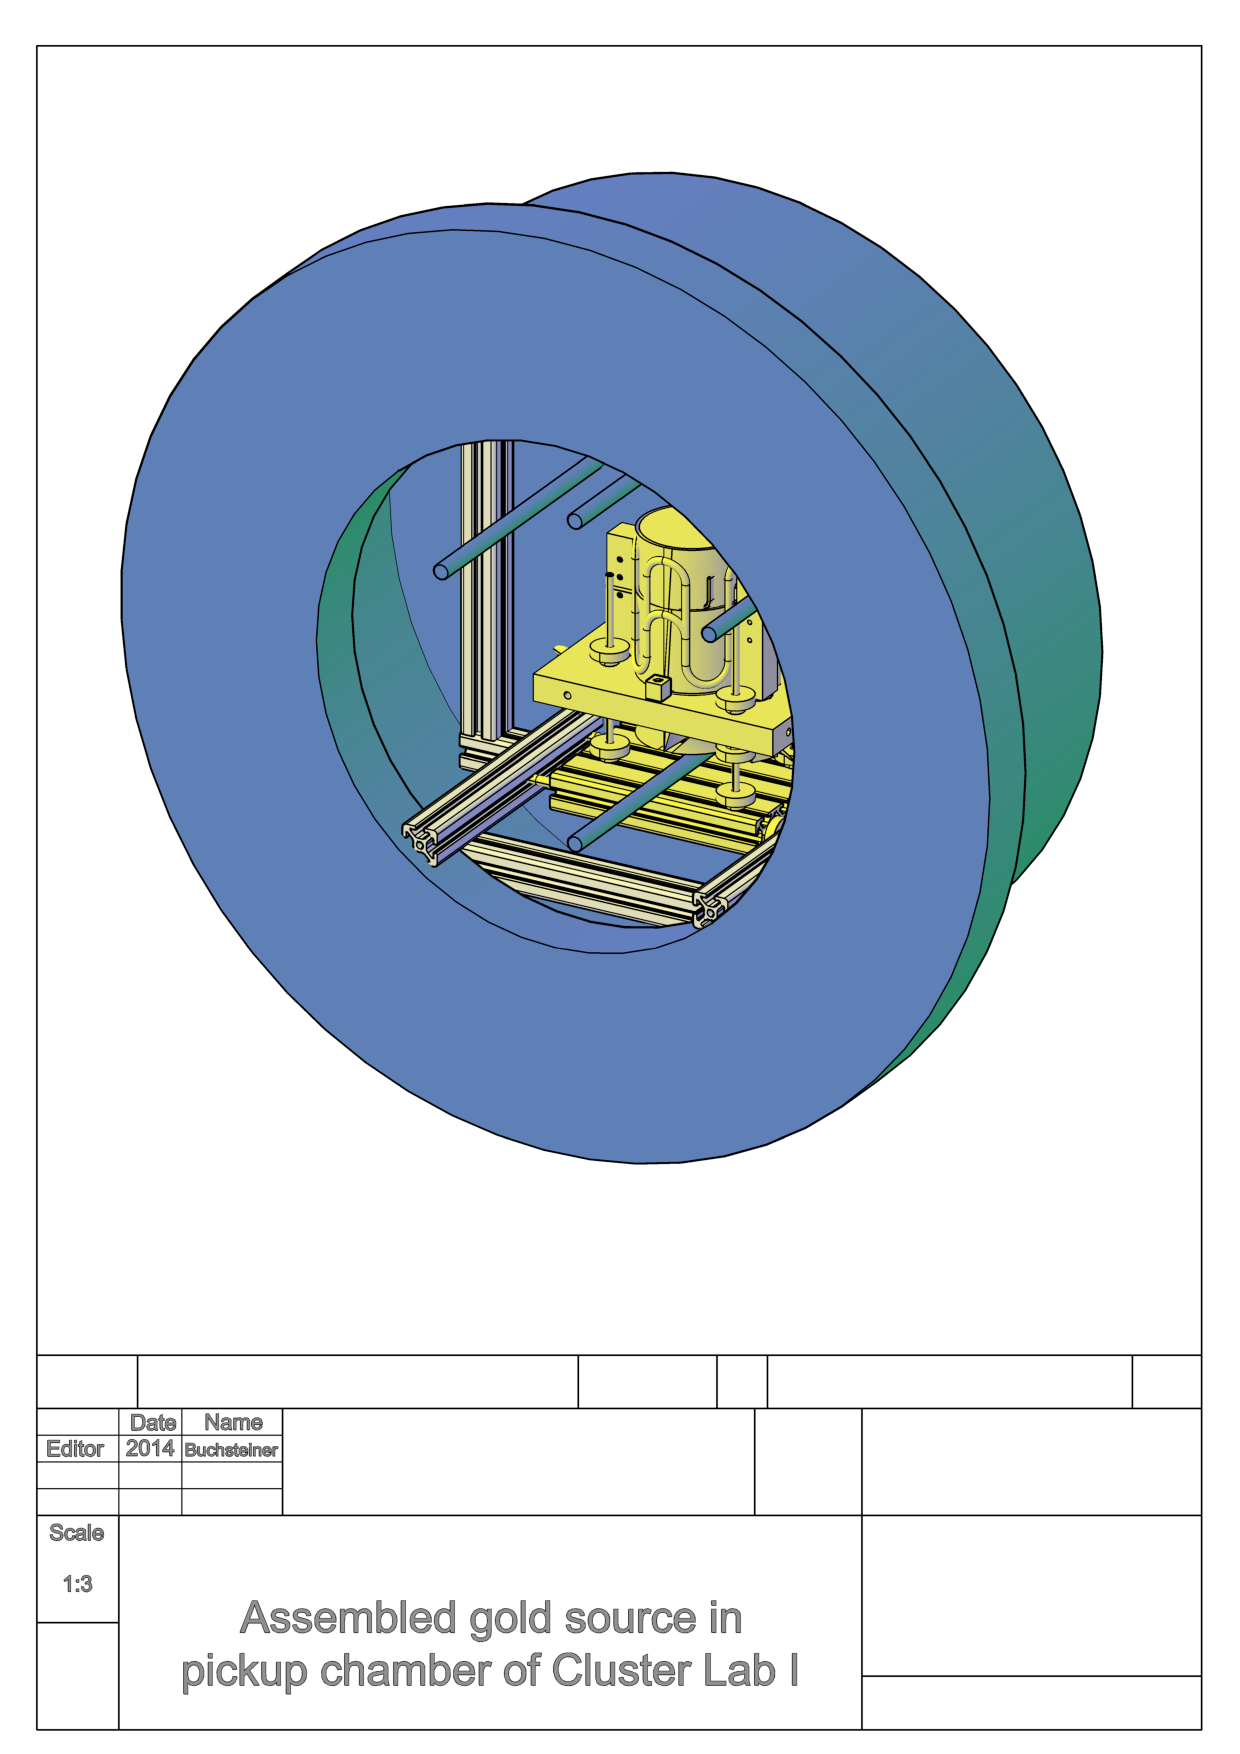
\includepdf[pages={1}]{img/technical-drawings/Aluminum_frame_oveninchamber_3D.pdf}

\includepdf[pages={1}]{img/technical-drawings/blank.pdf}
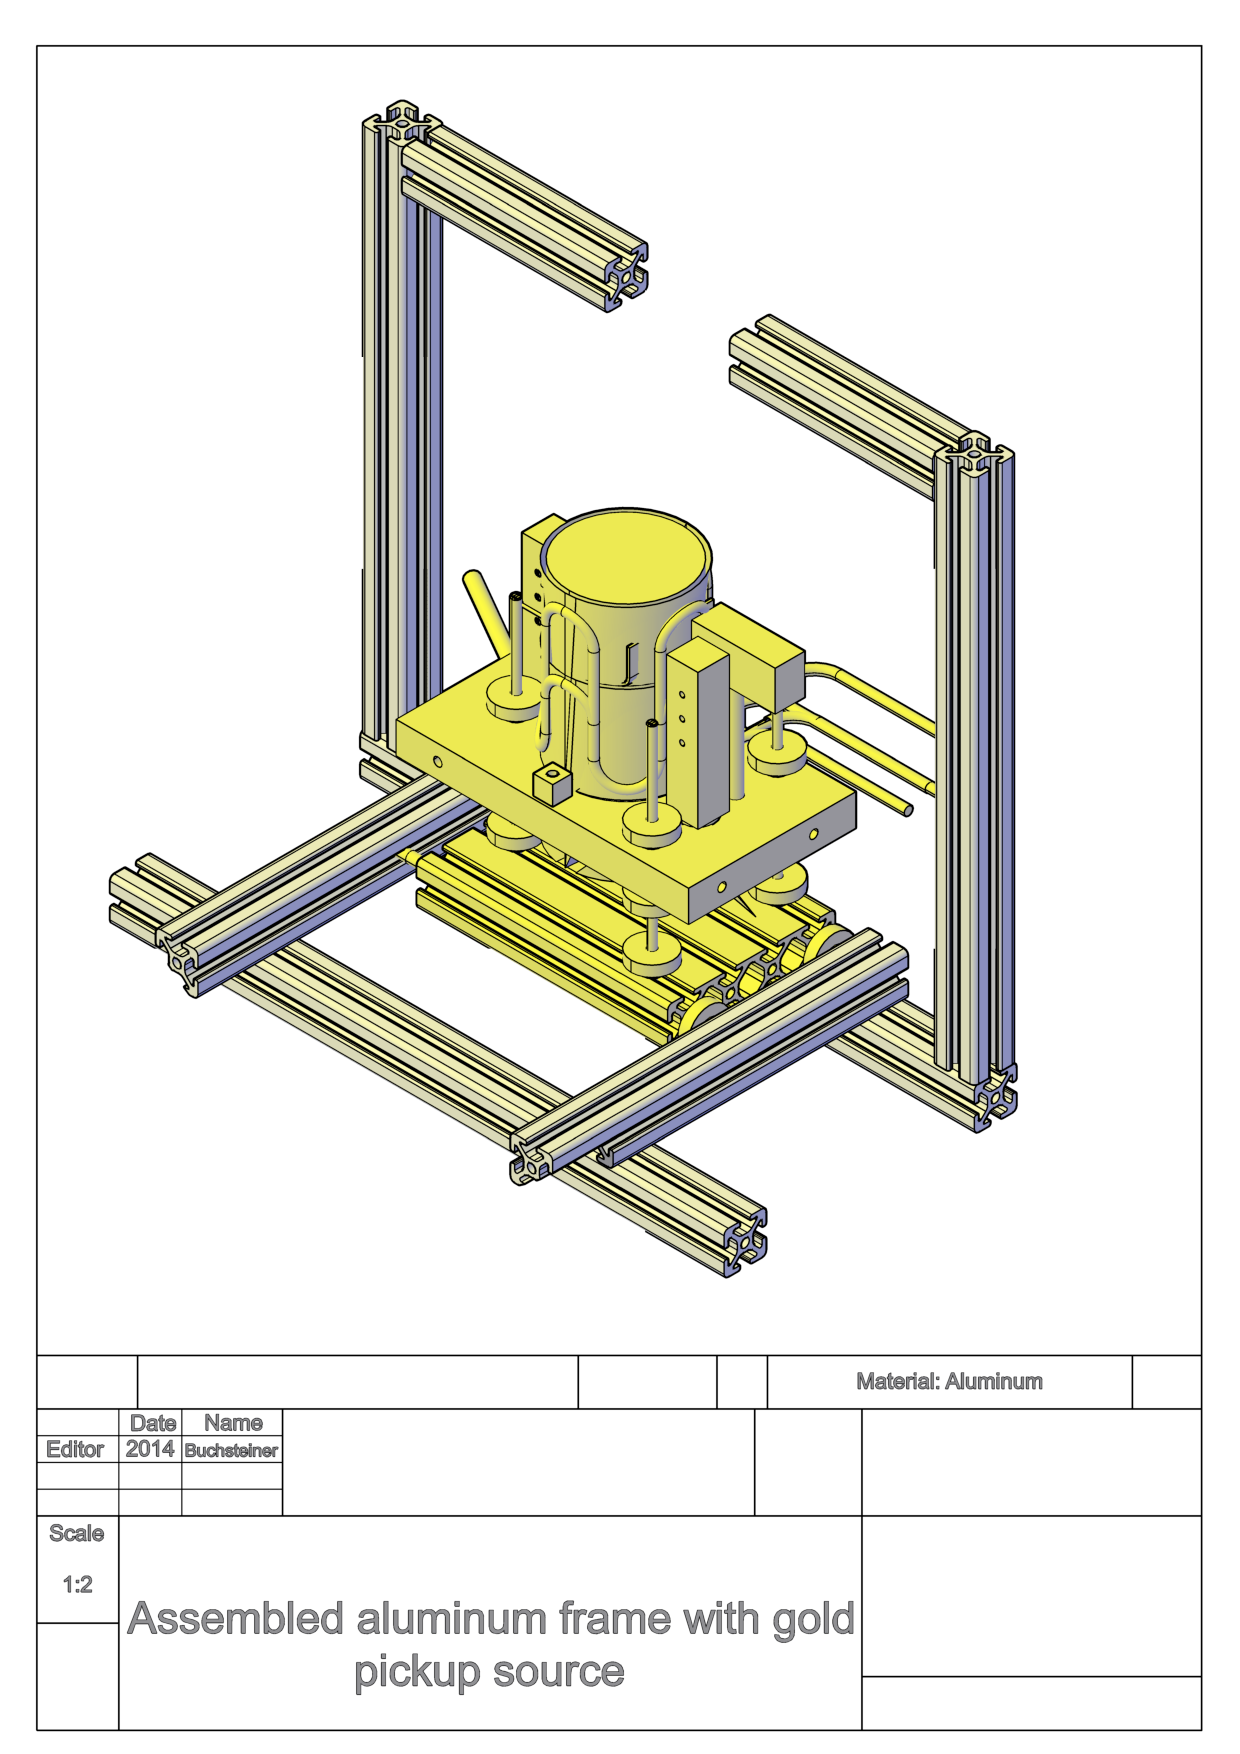
\includepdf[pages={1}]{img/technical-drawings/Aluminum_frame_oven_3D.pdf}

\includepdf[pages={1}]{img/technical-drawings/blank.pdf}
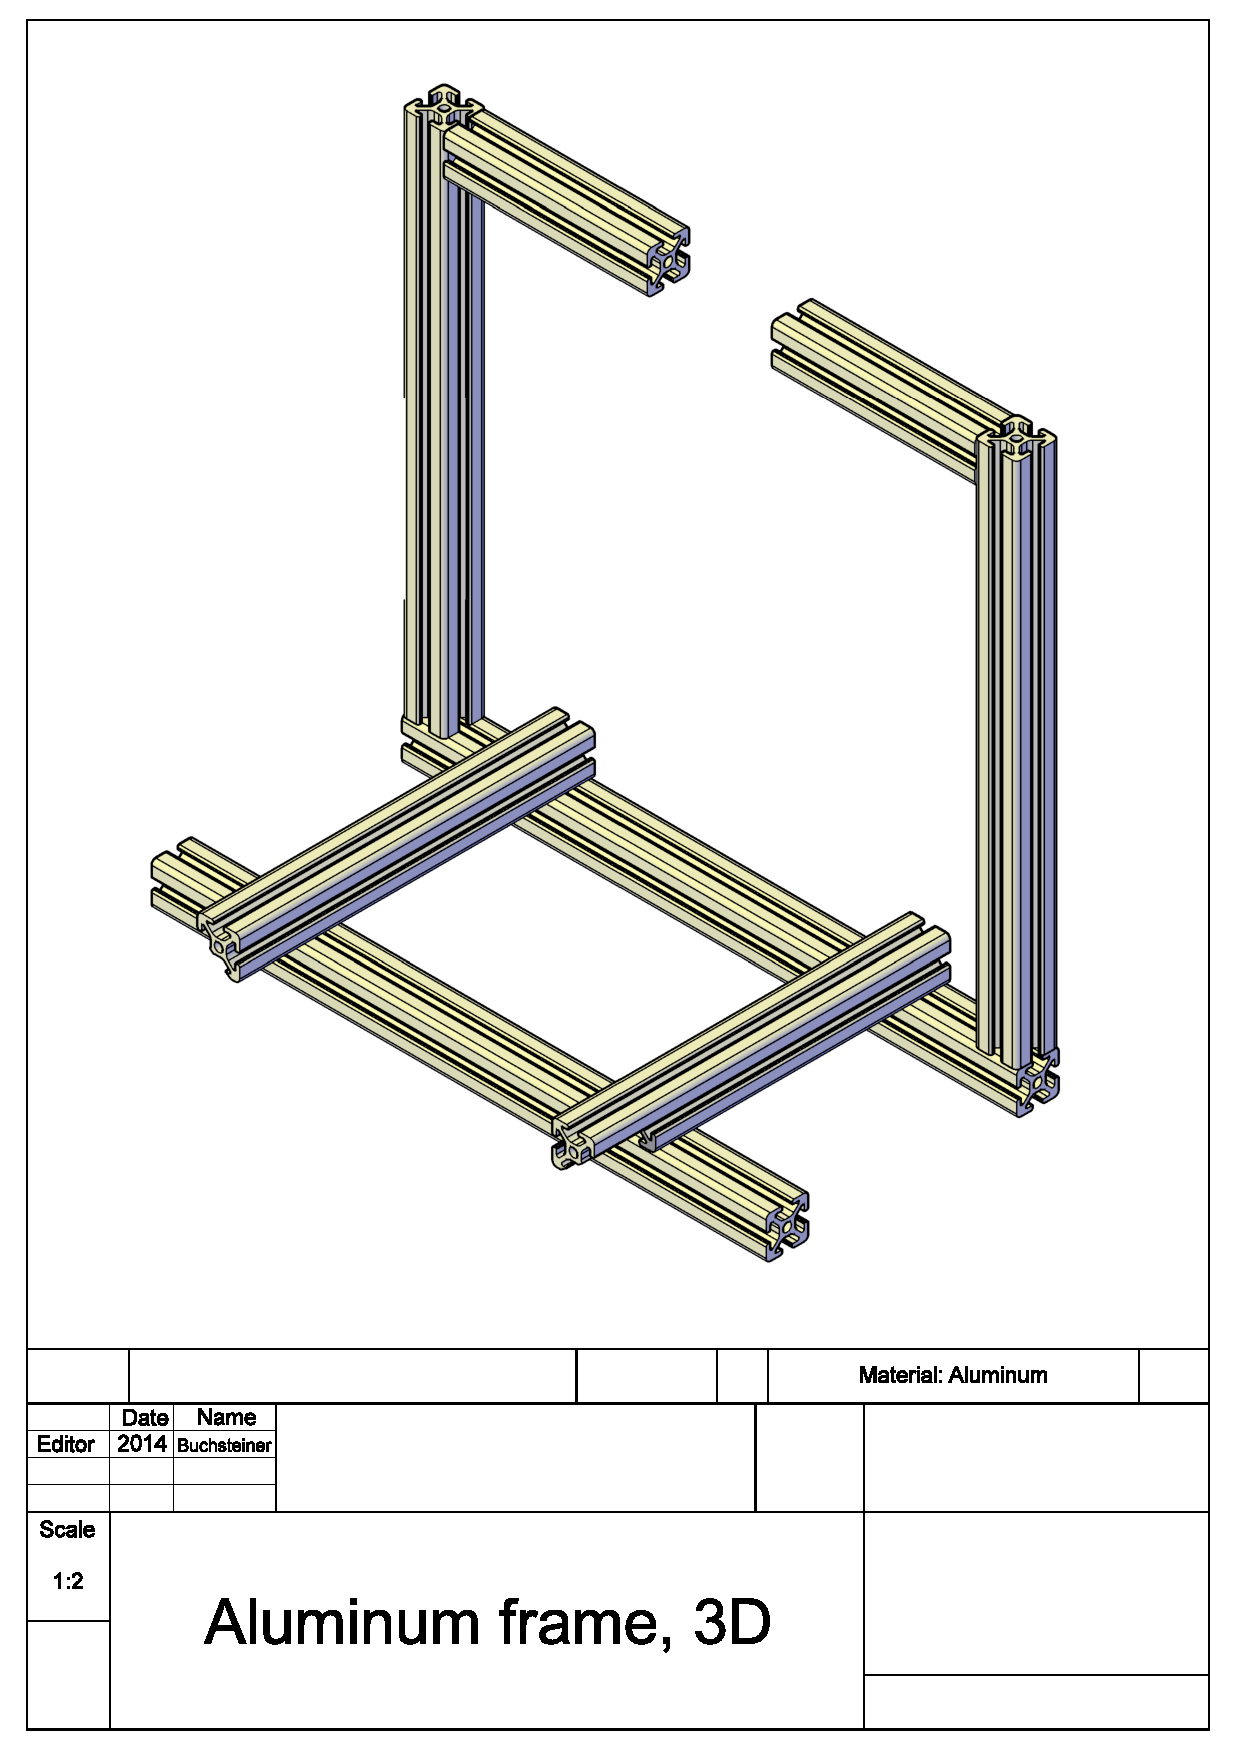
\includepdf[pages={1}]{img/technical-drawings/Aluminum_frame_3D.pdf}

\includepdf[pages={1}]{img/technical-drawings/blank.pdf}
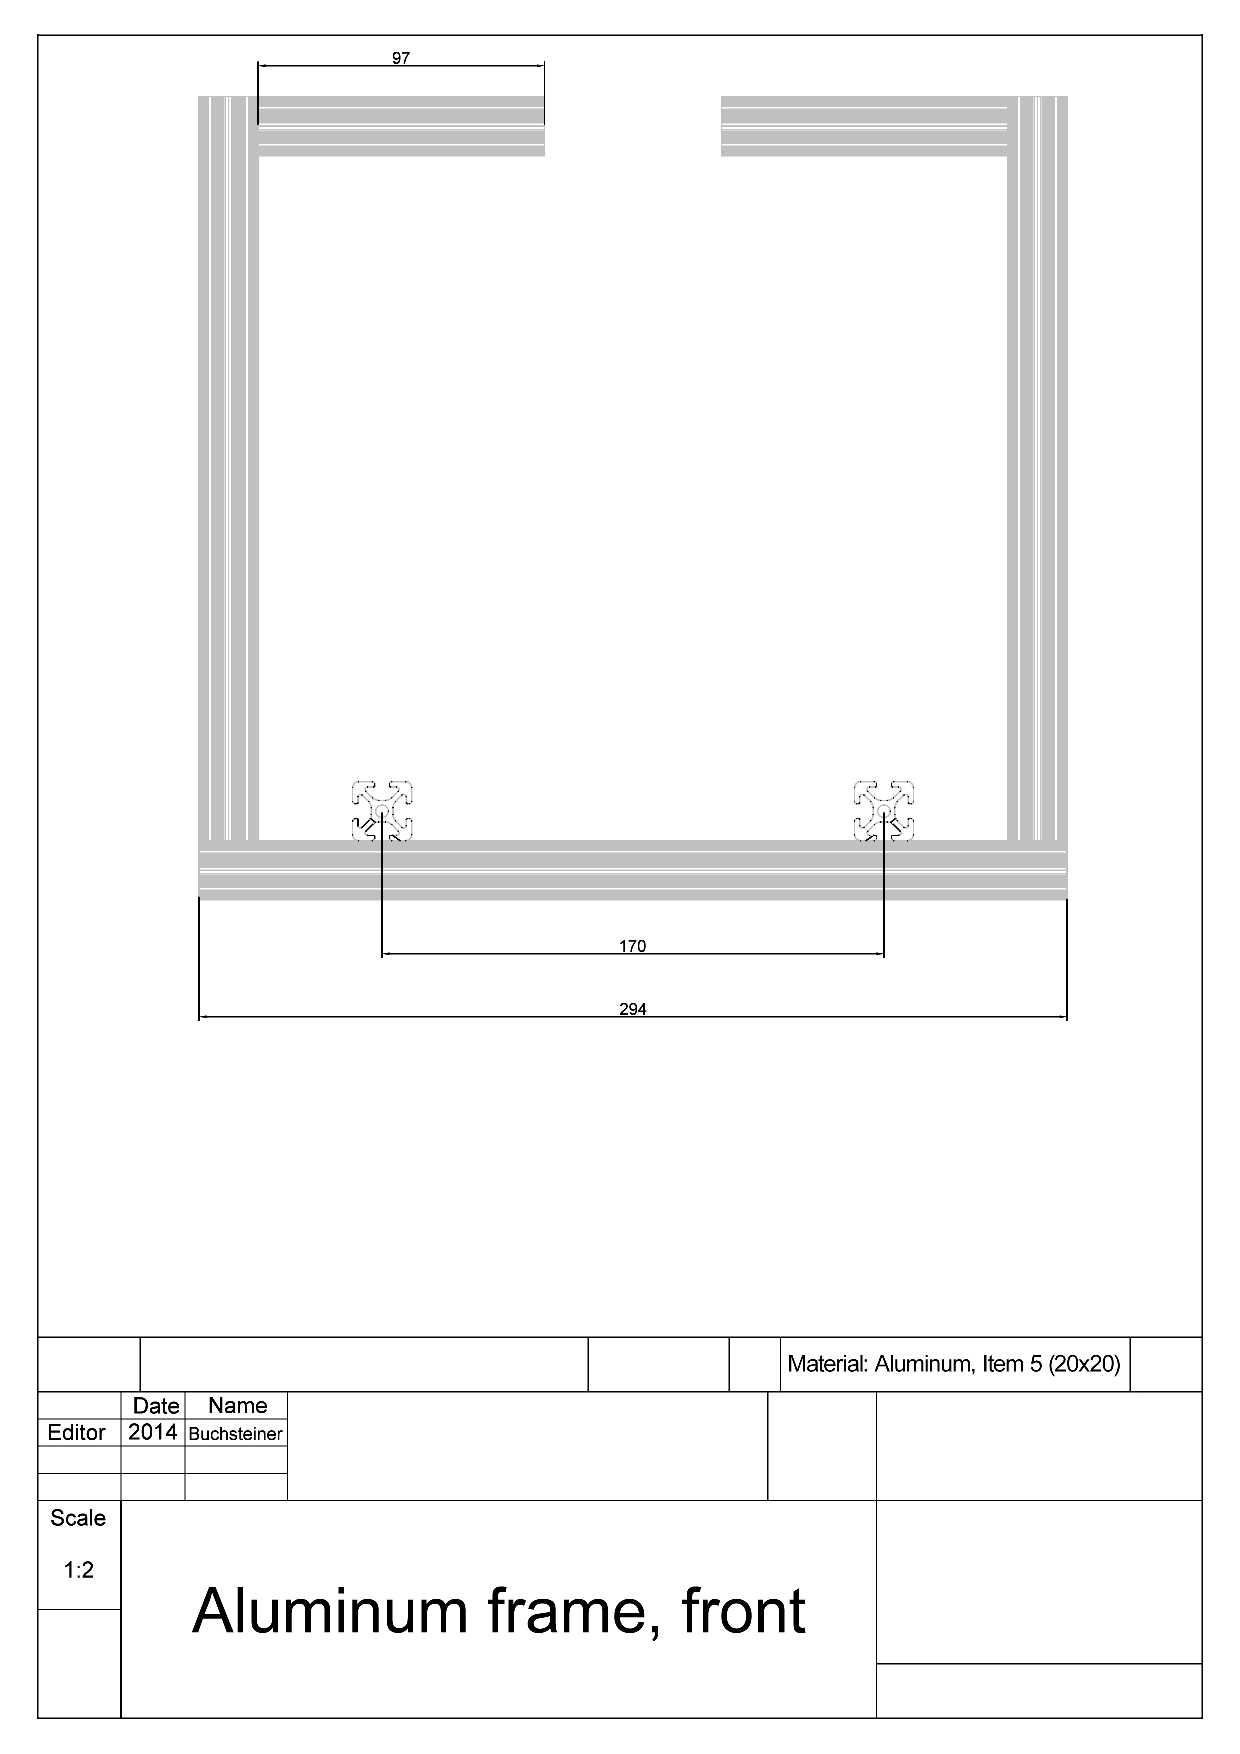
\includepdf[pages={1}]{img/technical-drawings/Aluminum_frame_front_ps.pdf}
\includepdf[pages={1}]{img/technical-drawings/blank.pdf}
\includepdf[pages={1}]{img/technical-drawings/Aluminum_frame_side.pdf}
\includepdf[pages={1}]{img/technical-drawings/blank.pdf}
\includepdf[pages={1}]{img/technical-drawings/Werkstatt_Aluprofile.pdf}
\includepdf[pages={1}]{img/technical-drawings/blank.pdf}
\includepdf[pages={1}]{img/technical-drawings/Werkstatt_Aluprofil_Einschnitt_ps.pdf}
\includepdf[pages={1}]{img/technical-drawings/blank.pdf}
\includepdf[pages={1}]{img/technical-drawings/Werkstatt_Winkel.pdf}
%\chapter{LabView Block Diagrams}


%%%%%% Manually add list of figures to TOC %%%%%%
\newpage
\phantomsection \label{listoffig}
\addcontentsline{toc}{chapter}{List of Figures}
\listoffigures

%%%%%% Manually add list of tables to TOC %%%%%%
\newpage
\phantomsection \label{listoftab}
\addcontentsline{toc}{chapter}{List of Tables}
\listoftables

%%%%%% Manually add bibliography to TOC %%%%%%
\newpage
\phantomsection \label{bibliography}
\addcontentsline{toc}{chapter}{Bibliography}

\bibliographystyle{unsrt}
\bibliography{MasterThesis.bib}


%%%%%% Manually add Acknow to TOC %%%%%%
\newpage
\phantomsection \label{acknow}
\addcontentsline{toc}{chapter}{Acknowledgments}
\titlespacing*{\chapter} {0pt}{30pt}{20pt}
\chapter*{Acknowledgments}
Now that I reached the point where it is time to write the very last page of my master thesis I would like to thank the people who supported me all the way: Thanks to my supervisor Prof. Ernst for giving me the opportunity to join your group and to witness what it's like to work in research as a physicist. I also want to thank Markus Koch to give me the idea of doing my thesis at this institute in the first place. \\
Philipp and Alex were very supportive during the assembly and installation of the gold pick up source. Thank you for that.

Special thanks go to G\"unter and Flo. It was a pleasure working with you guys. Thank you G\"unter for making countless nights in our lab informative and fun at the same time and for patently answering my questions. Hit your ''climate thing'' and make our world a better place. Thank you Flo for the greatest support whilst writing this thesis I can ever wish for. Keep up your inspiring enthusiasm and all the best for your, without doubt, great scientific career.

Of course I also want to thank my friends beside work: Thank you Delia for your great help in all that theoretical stuff. You brought me eureka moments not only once. \\
Thank you Bertram. Without you my first semester would have been terrible and most likely I would never have passed it. I miss the time sitting in my kitchen, learning analysis and only talking about mountainbikes. \\
Thank you Fritz for being such a great friend. For listening to all my problems, no matter if small or big, always having an open ear for stupid ideas and never judging me for anything. I will always remember our years of study with a smile - also because of you.

Danke an meine Familie, die mir in schwierigen Zeiten immer den R\"ucken gest\"arkt hat und ohne die mein Studium, so nicht m\"oglich gewesen w\"are.

Thank you Babs. The last few years with you by my side were the greatest in my life. Sorry for always being so busy and sometimes living in a world so far, far away. I appreciate your support so much. I love you.


\end{document}
